\documentclass[a4paper, oneside, 11pt]{article}

\usepackage[english]{babel}
\usepackage[T1]{fontenc}

\usepackage[a4paper,top=2.5cm,bottom=2.5cm,left=2cm,right=2cm]{geometry}

\usepackage{amsmath}
\usepackage{graphicx}
\usepackage{fancyhdr}
\usepackage{float}
\usepackage[labelfont=bf]{caption}
\usepackage{subcaption}
\usepackage{comment}
\usepackage{lastpage}
\usepackage{siunitx}
\usepackage{csquotes}
\usepackage{amsfonts}
\usepackage{textcomp}
\usepackage{hyperref}
\usepackage{indentfirst}

\allowdisplaybreaks

\pagestyle{fancy}
\fancyhf{}
\rhead{Filtering}
\lhead{Digital Signal Processing}
\cfoot{Page  \thepage \hspace{1pt} of \pageref{LastPage}}
\setlength{\headheight}{14pt}

\begin{document}

\begin{titlepage}
	\begin{center}
		\begin{figure}[htb!]
			\centering
				
\includegraphics[width=10cm]{figures/istlogo.jpg}
		\end{figure}
        
        \LARGE{\textbf{Instituto Superior Técnico}}\\
        \vspace{20pt}
        \Large{Integrated Masters in Aerospace Engineering}\\
        \vspace{10pt}
        \Large{Digital Signal Processing}\\
        \vspace{10pt}
        \Large{2\textsuperscript{nd} Semester 2020/2021}\\
            
        \vspace{40pt}
        \noindent\rule{15cm}{1pt}\\
        \Huge{\center \textbf{Laboratory 3}} 
        \par 
        \Huge{\center \textbf{Filtering}}\\
        \noindent\rule{15cm}{1pt}\\
        
        \vspace{60pt}
        \large{\begin{tabular}{ll}
            \textbf{Group 40:} & \textbf{Professor:} \\
            89683, José Neves & Prof. Rita Cunha\\
            89691, Leonardo Pedroso \hspace{1cm} & \\
        \end{tabular}}
    
        \vspace{60pt}
        \large{\today}
	\end{center}
\end{titlepage}

\newpage
\pagenumbering{arabic}
\setcounter{page}{1}


\section{R1. Observation of the corrupted signal}\label{sec:R1}

\subsection{R1.a) Original sound file}
First of all the signal from the sound file \texttt{fugee.wav} was loaded and heard. It is the song \textit{Killing Me Softly With His Song} by \textit{Fugees}. Furthermore, sharp impulsive noise is heard at particular time instants, which simulates the noise that typically corrupts old vinyl records.

\subsection{R1.b) Time domain analysis of original signal}
Second, the sound signal is analyzed in the time domain. Fig. \ref{fig:R1b} shows the evolution of a segment of the signal with time. The sharp impulsive noise heard and described in the previous section is very noticeable in this figure. The noise seems to be modeled by an impulse.
\begin{figure}[htbp]
	\centering
	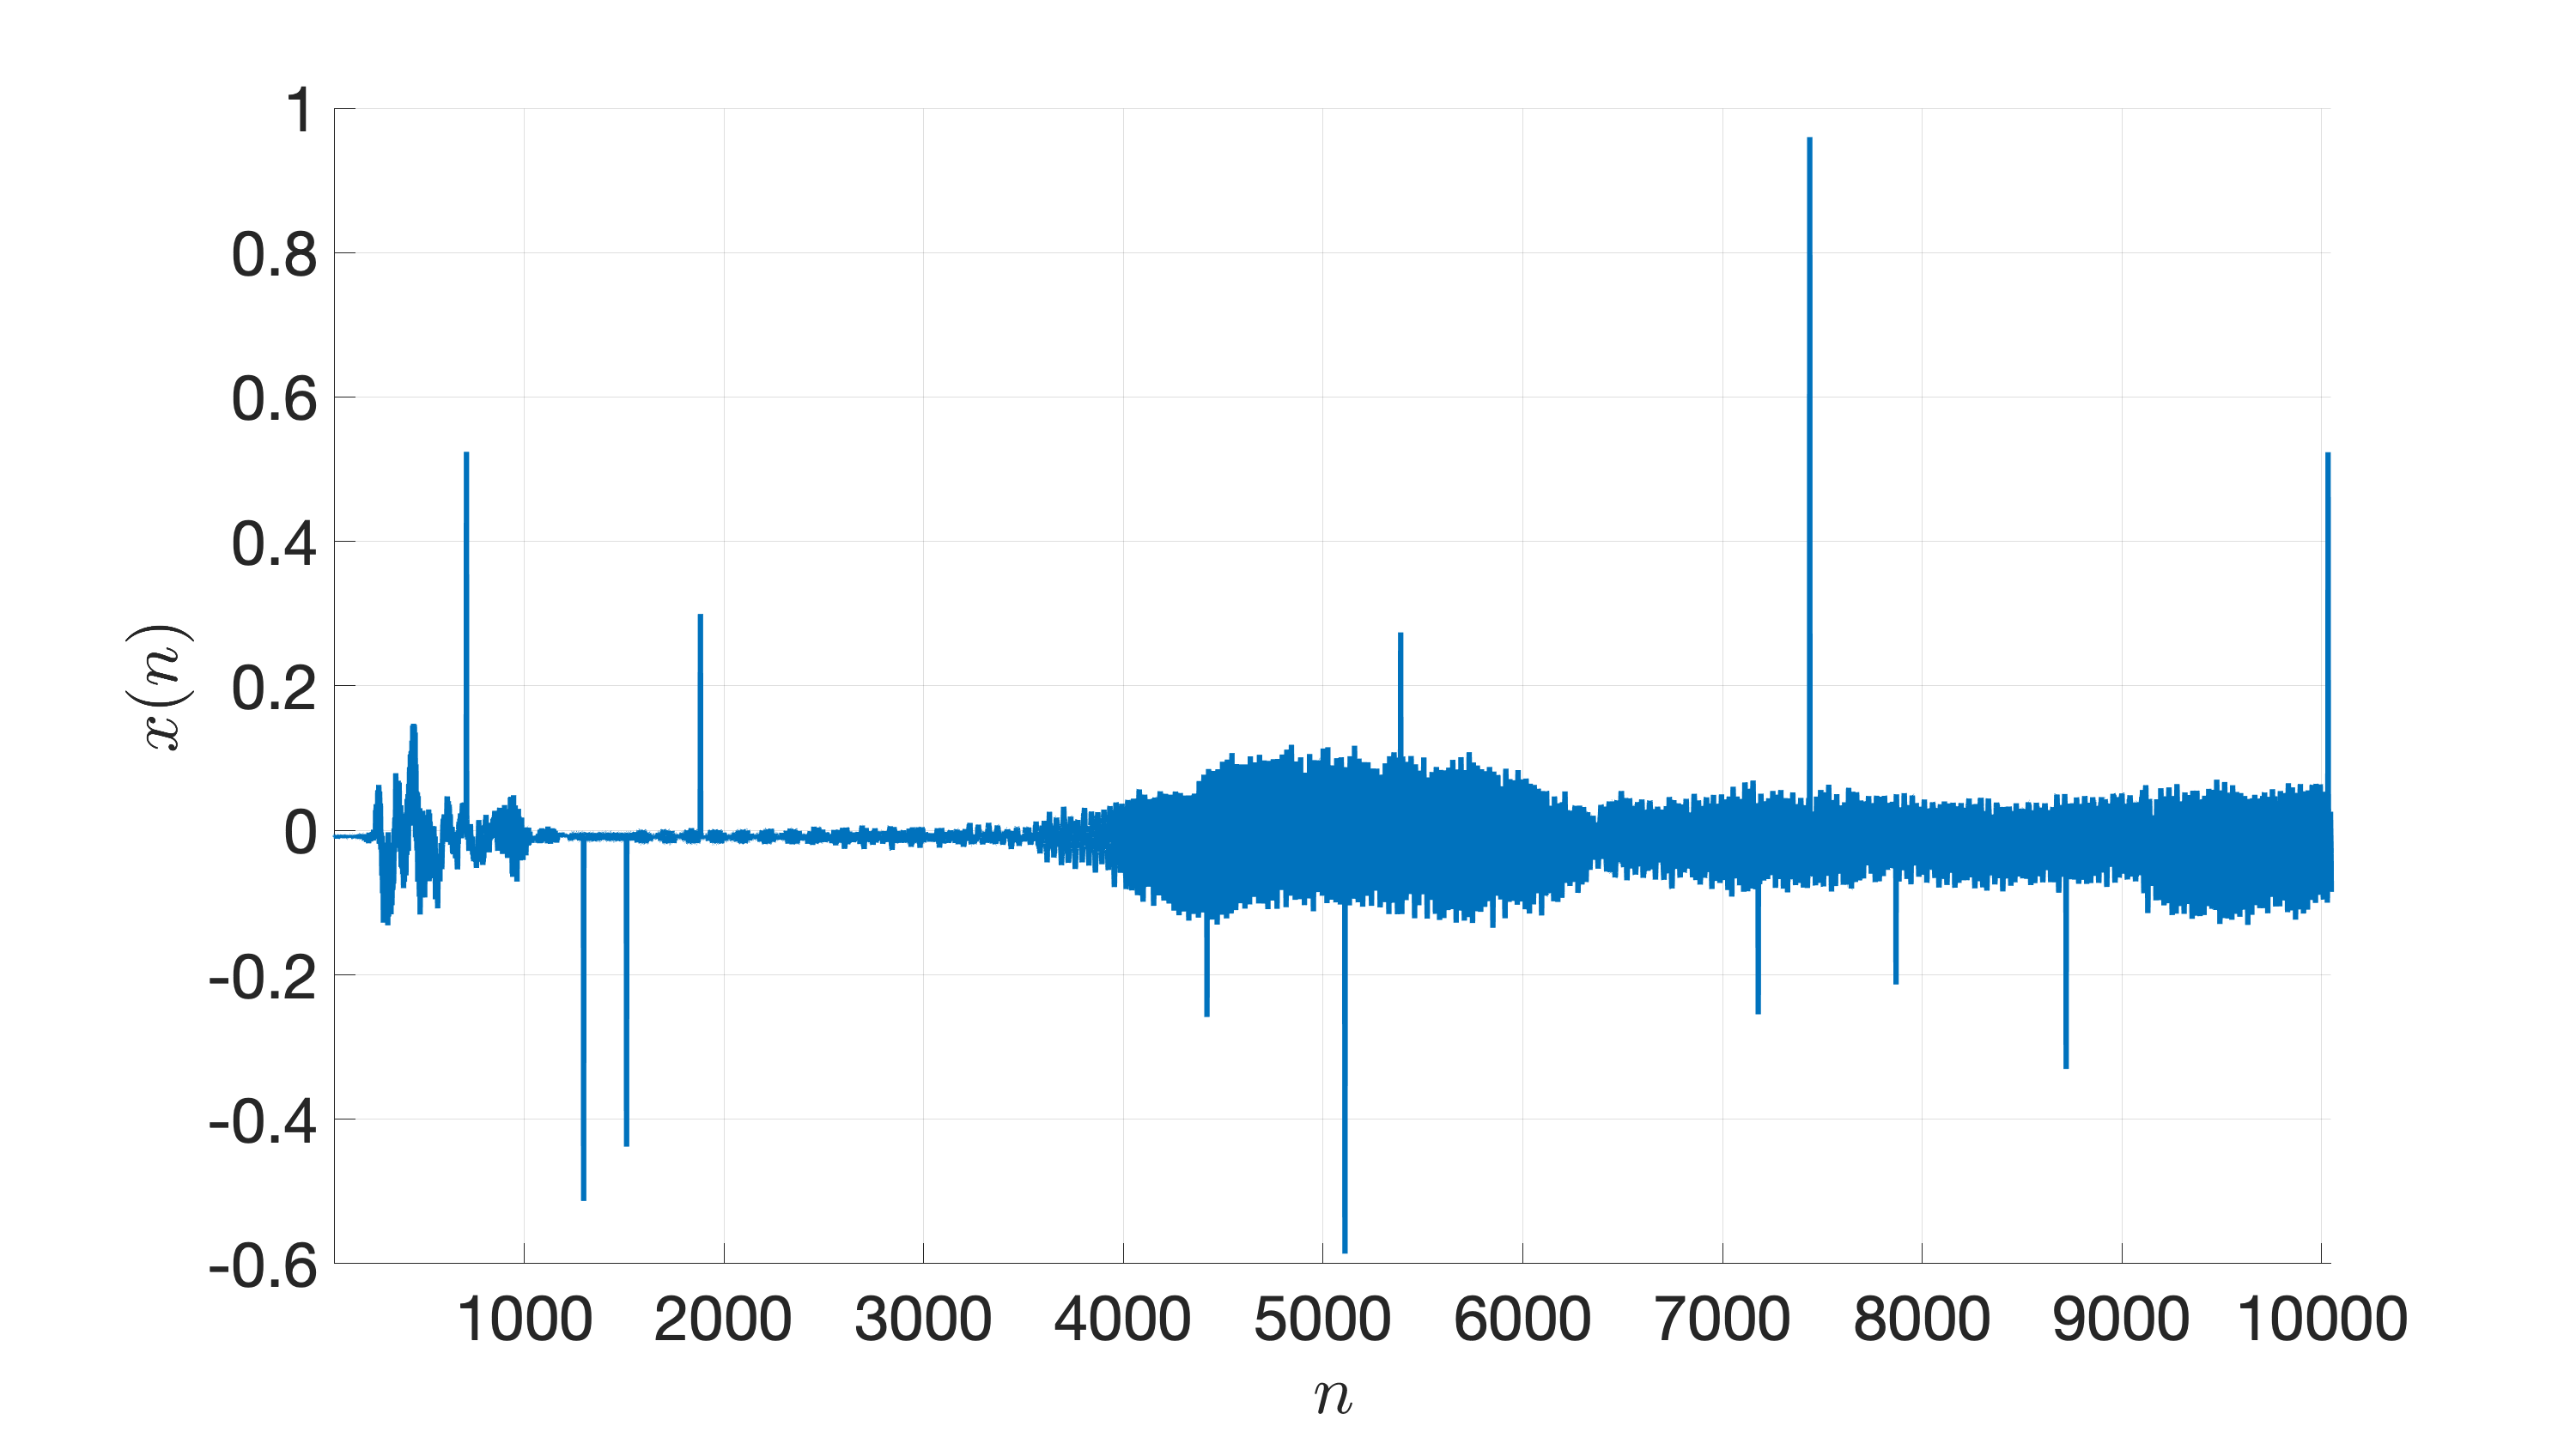
\includegraphics[width= 0.8\textwidth]{figures/R1b.png}
	\caption{Segment of the original sound signal in the time domain.}
	\label{fig:R1b}
\end{figure}

\subsection{R1.c) Frequency domain analysis of original signal}
Third, the sound signal is analyzed in the frequency domain. Fig. \ref{fig:R1c} shows the magnitude spectrum of the original signal. It shows the original sound signal has a broad frequency spectrum. Nevertheless, there is not clear evidence about the presence of noise in this plot. In fact, given that the noise is impulsive, its magnitude representation is a constant, thus it is very difficult to detect when superimposed with the spectrum of the song. As a matter of fact, the spectrogram of the segment of the sound plotted in Fig. \ref{fig:R1b} is shown in Fig. \ref{fig:R1c_spectrogram}. Contrarily to the magnitude spectrum of the signal, the sprectrogram gives insight into the characteristics of the noise, since it is possible to distinguish the frequency composition at separate time instants, allowing to identify the noise impulses as vertical lines of constant magnitude across all frequencies. It is possible to notice that, as predicted, the instants for which there is impulsive noise correspond to a constant spectrum across all frequencies. It is concluded that, while it is very easy to identify impulsive noise in the time domain, the opposite happens in the frequency domain. This fact hints that a filter suitable to filter such noise should operate in the time domain instead of the frequency domain.
\begin{comment}
\begin{figure}[htbp]
	\centering
	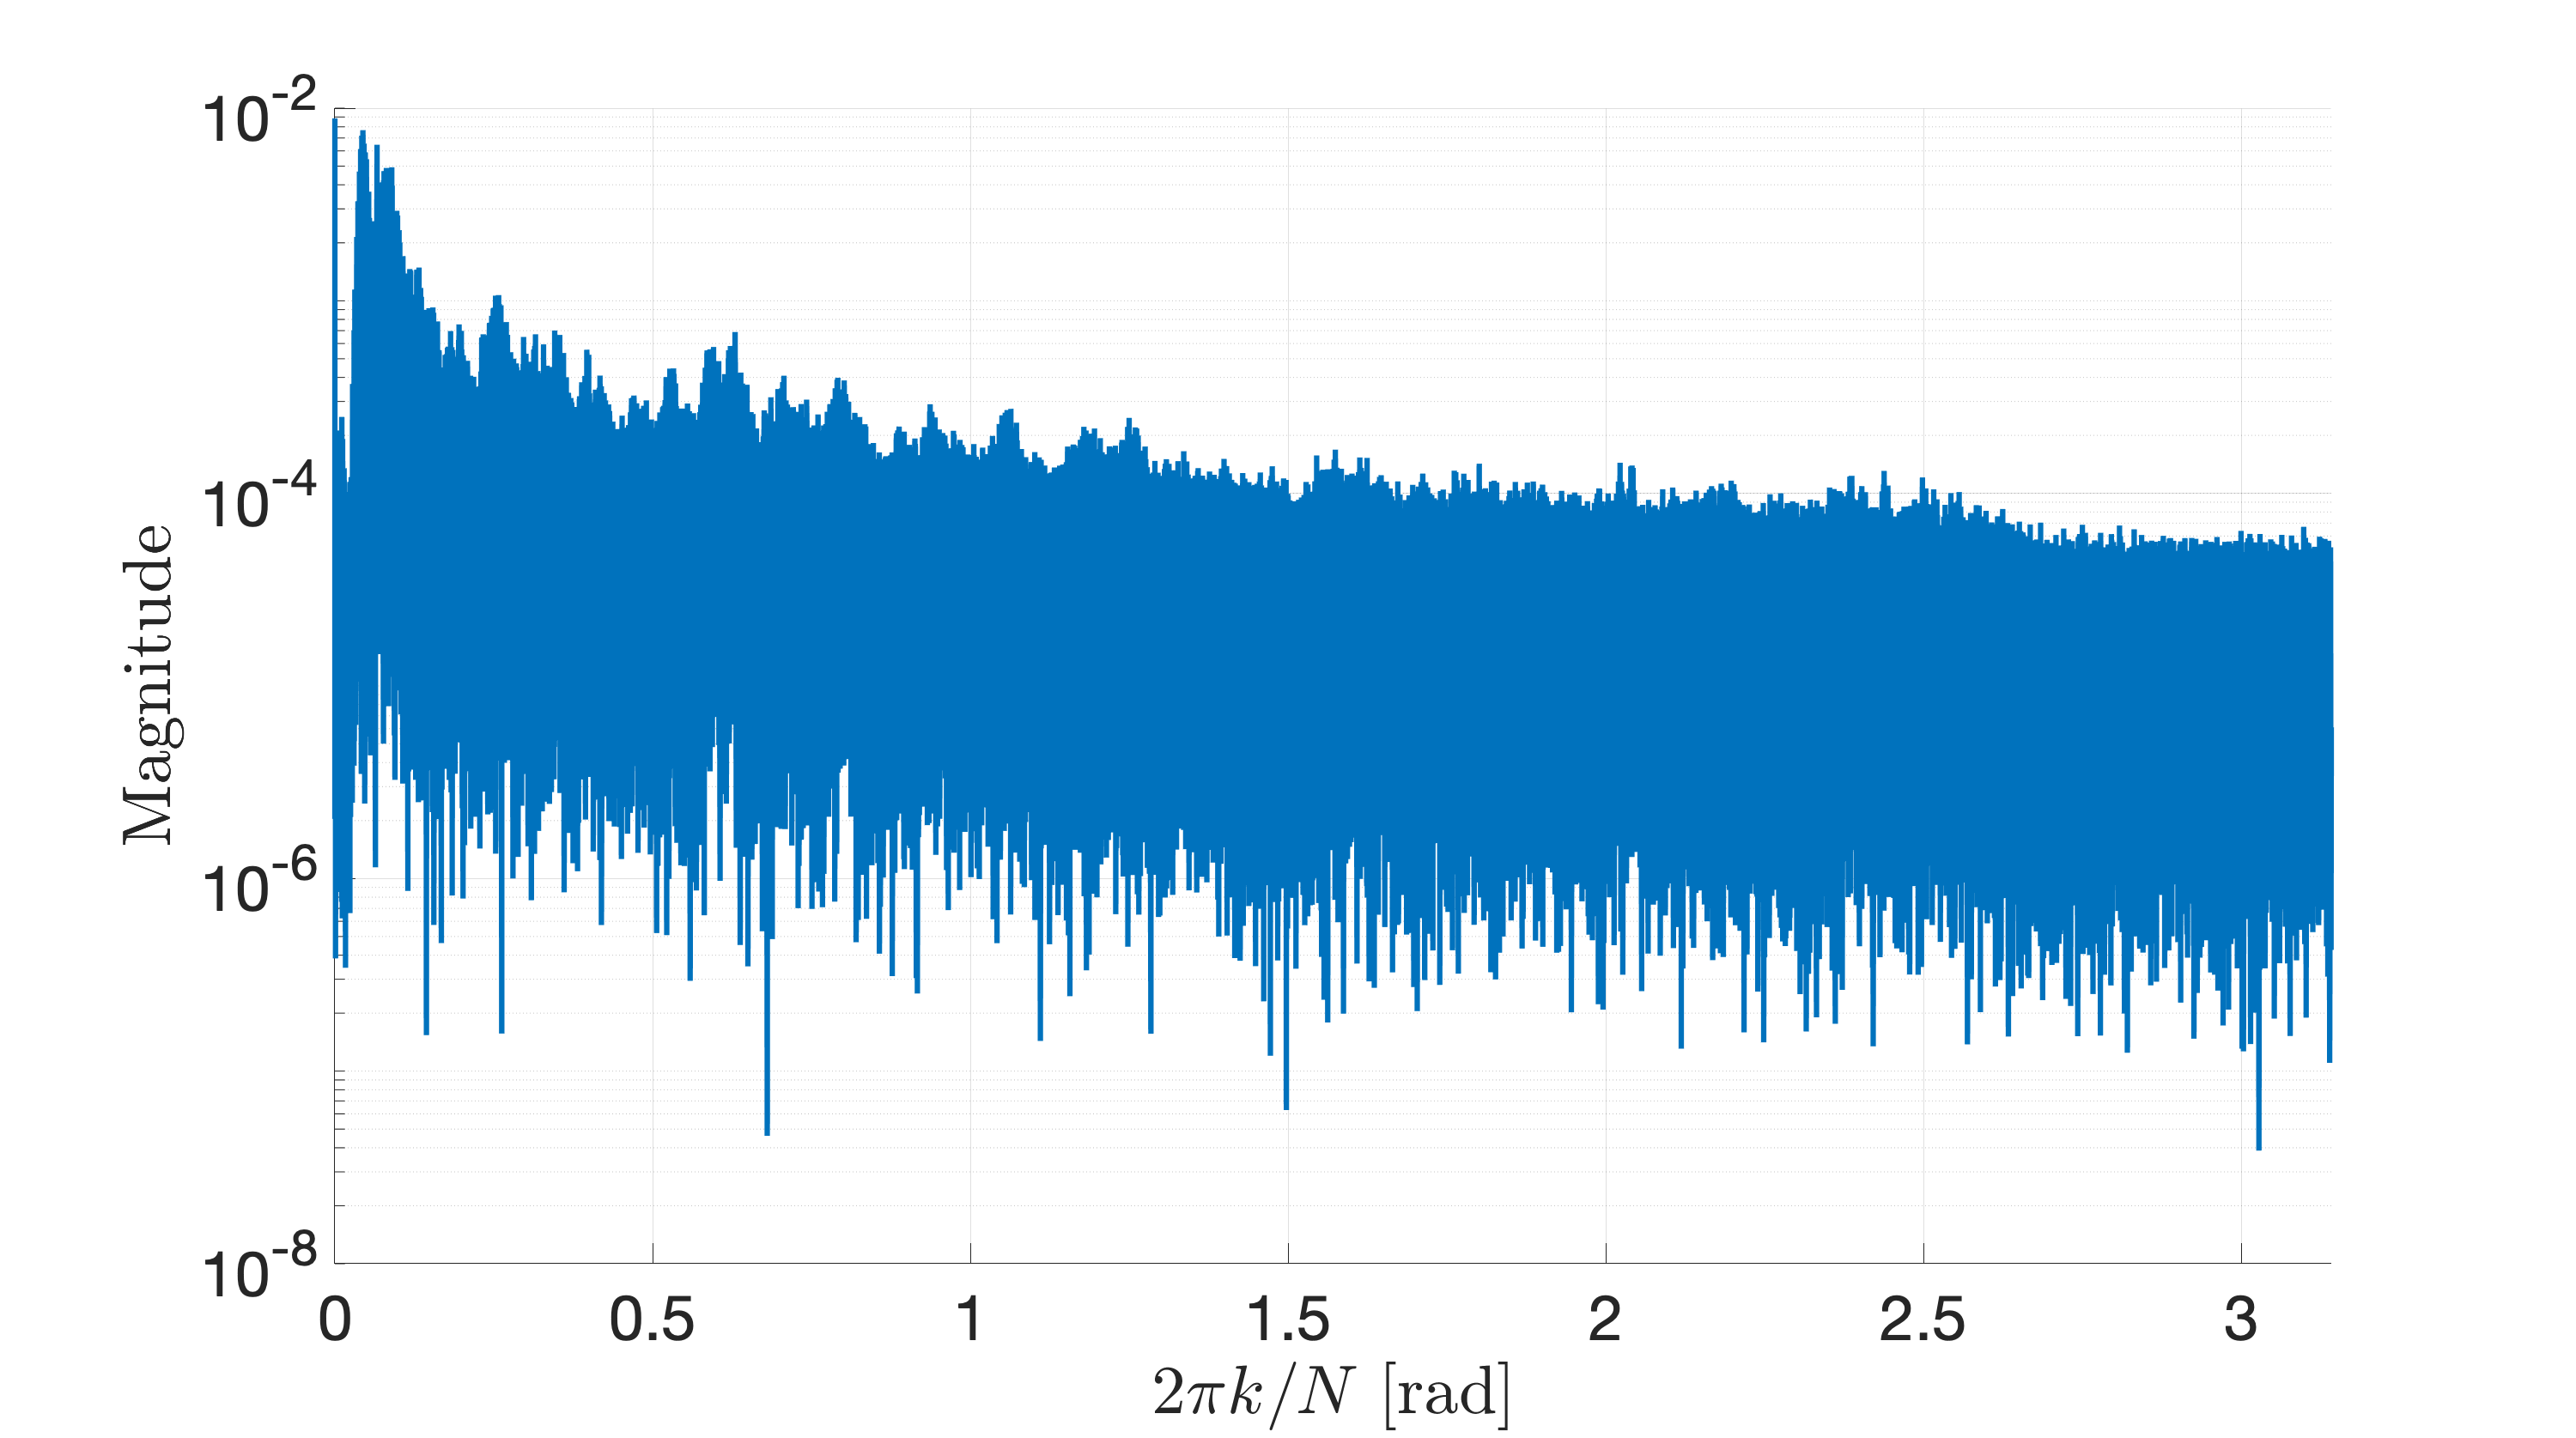
\includegraphics[width= 0.8\textwidth]{figures/R1c.png}
	\caption{Magnitude spectrum of the original sound signal.}
	\label{fig:R1c}
\end{figure}
\begin{figure}[htbp]
	\centering
	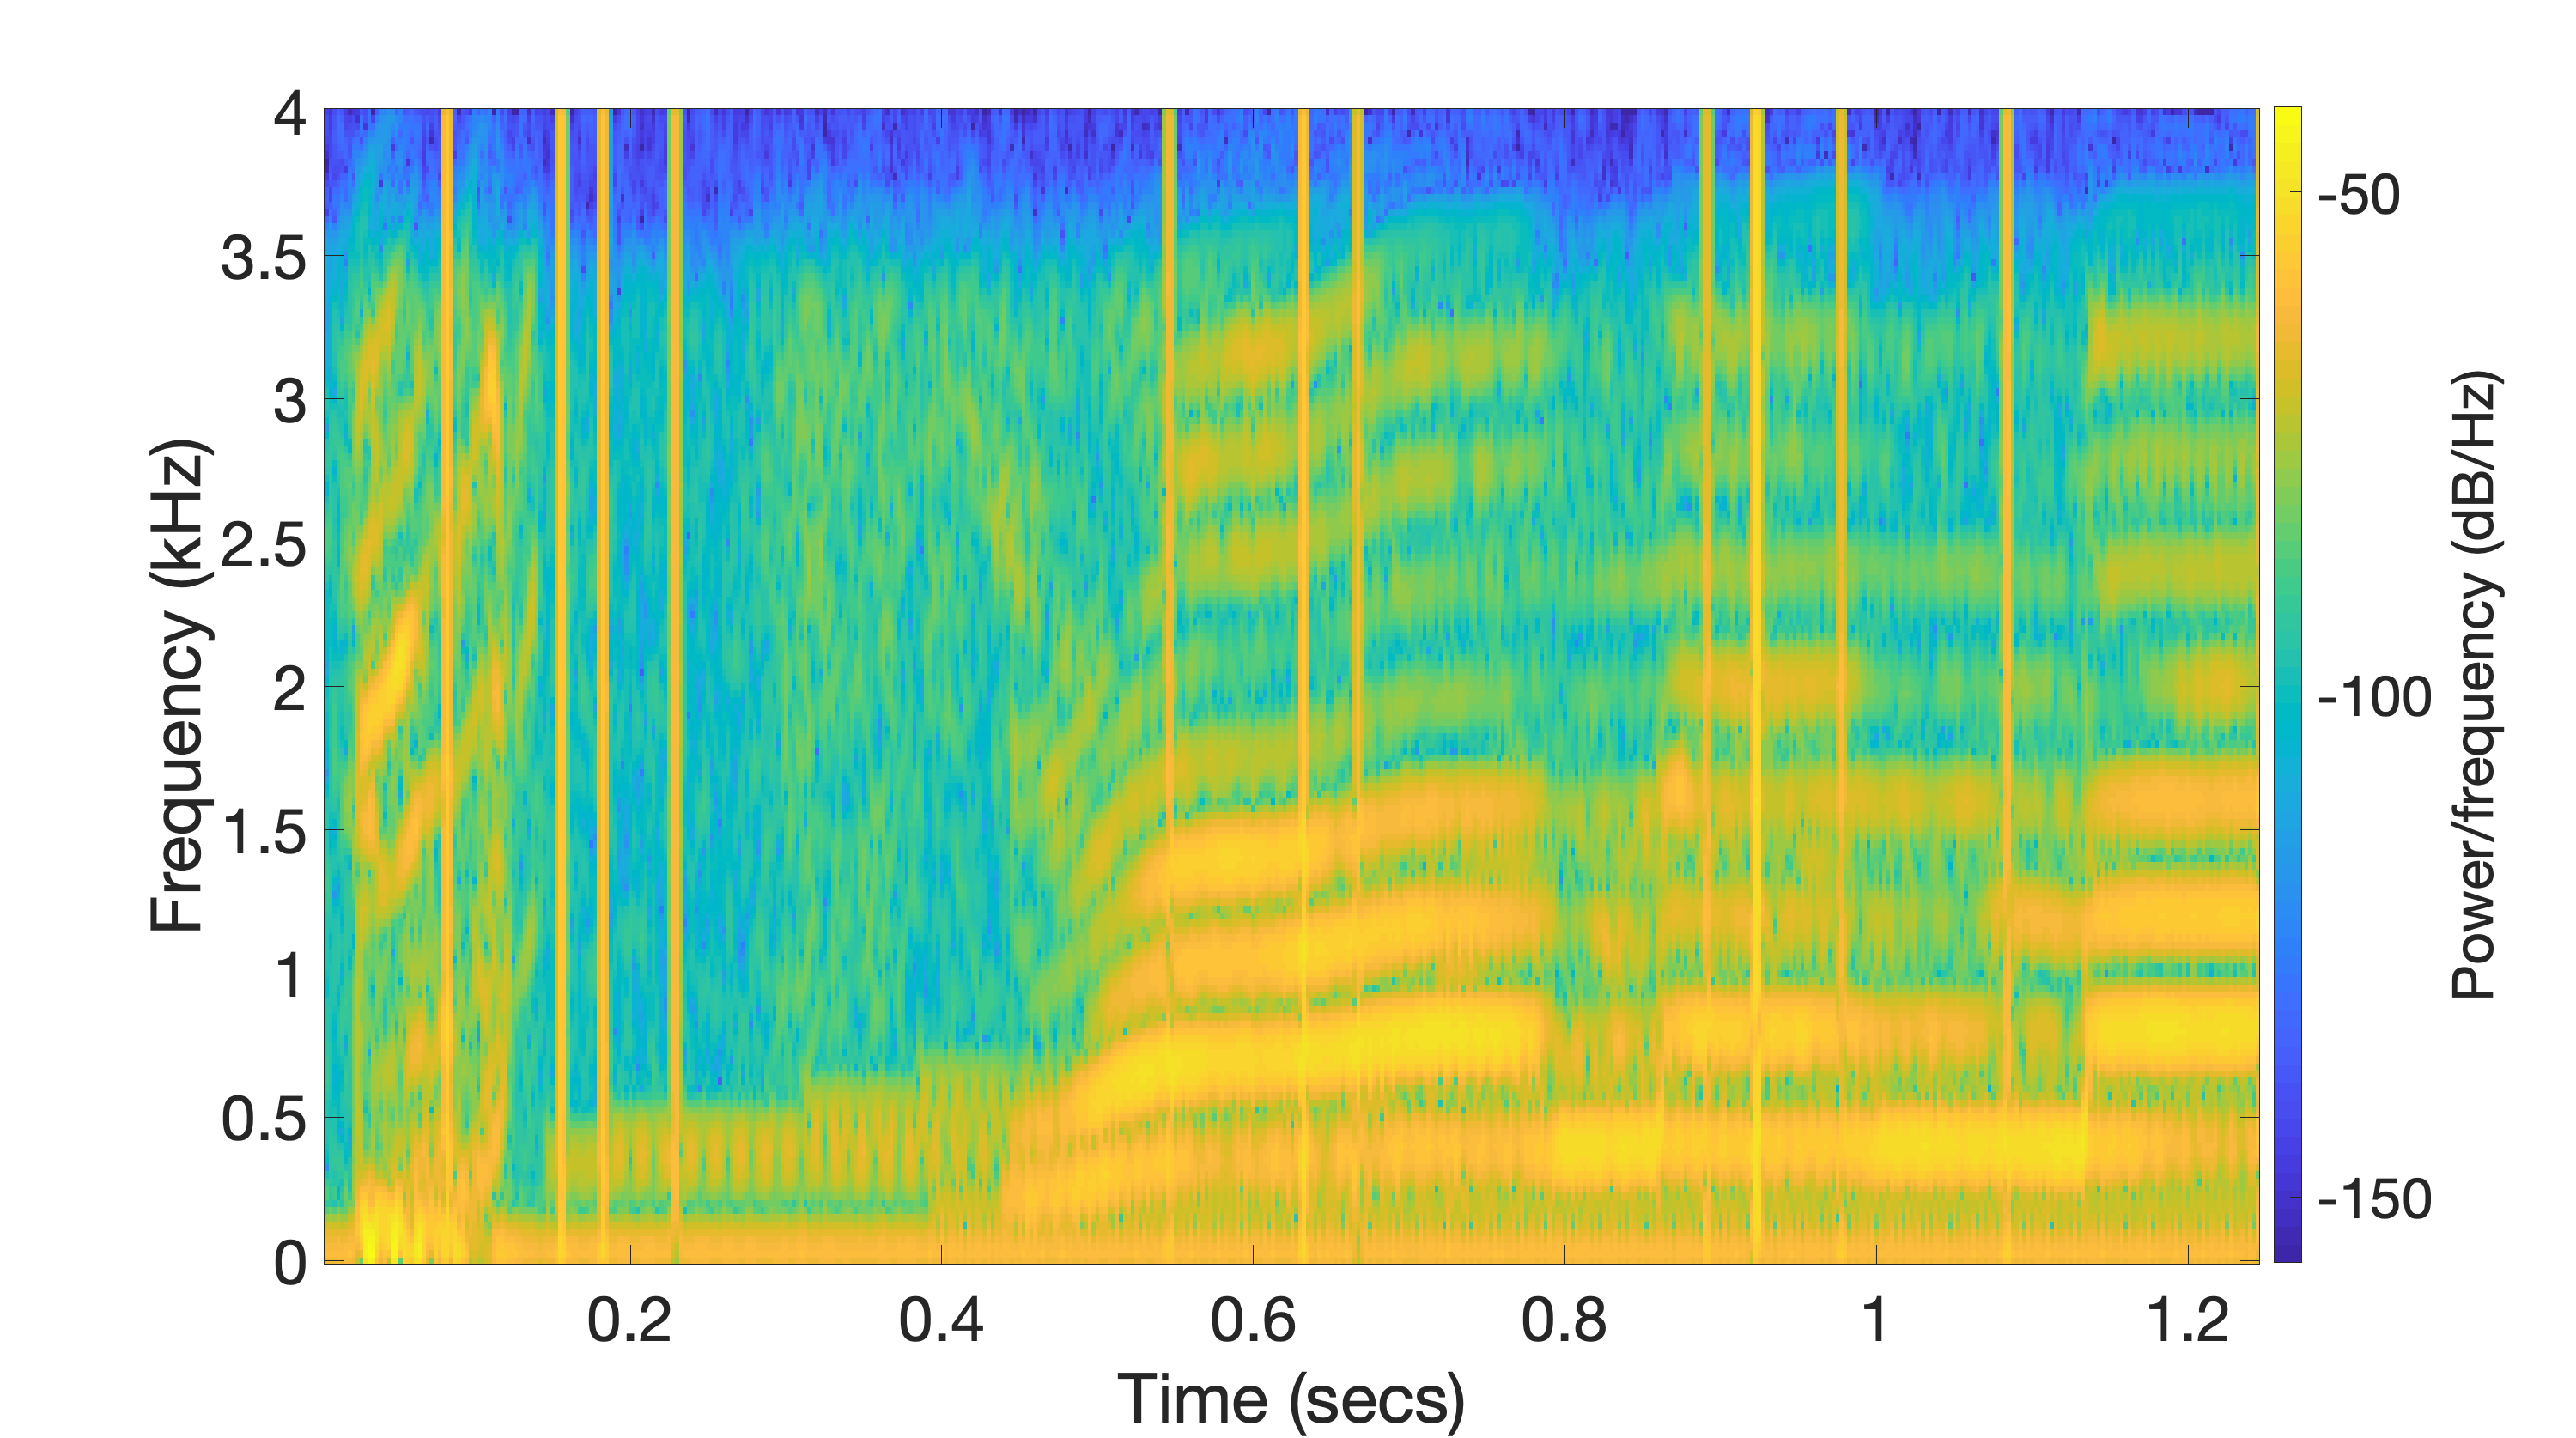
\includegraphics[width= 0.8\textwidth]{figures/R1c_spectrogram.png}
	\caption{Spectrogram.}
	\label{fig:R1c_spectrogram}
\end{figure}
\end{comment}
\begin{figure}[htbp]
	\centering
	\begin{minipage}[b]{.49\textwidth}
		\centering
		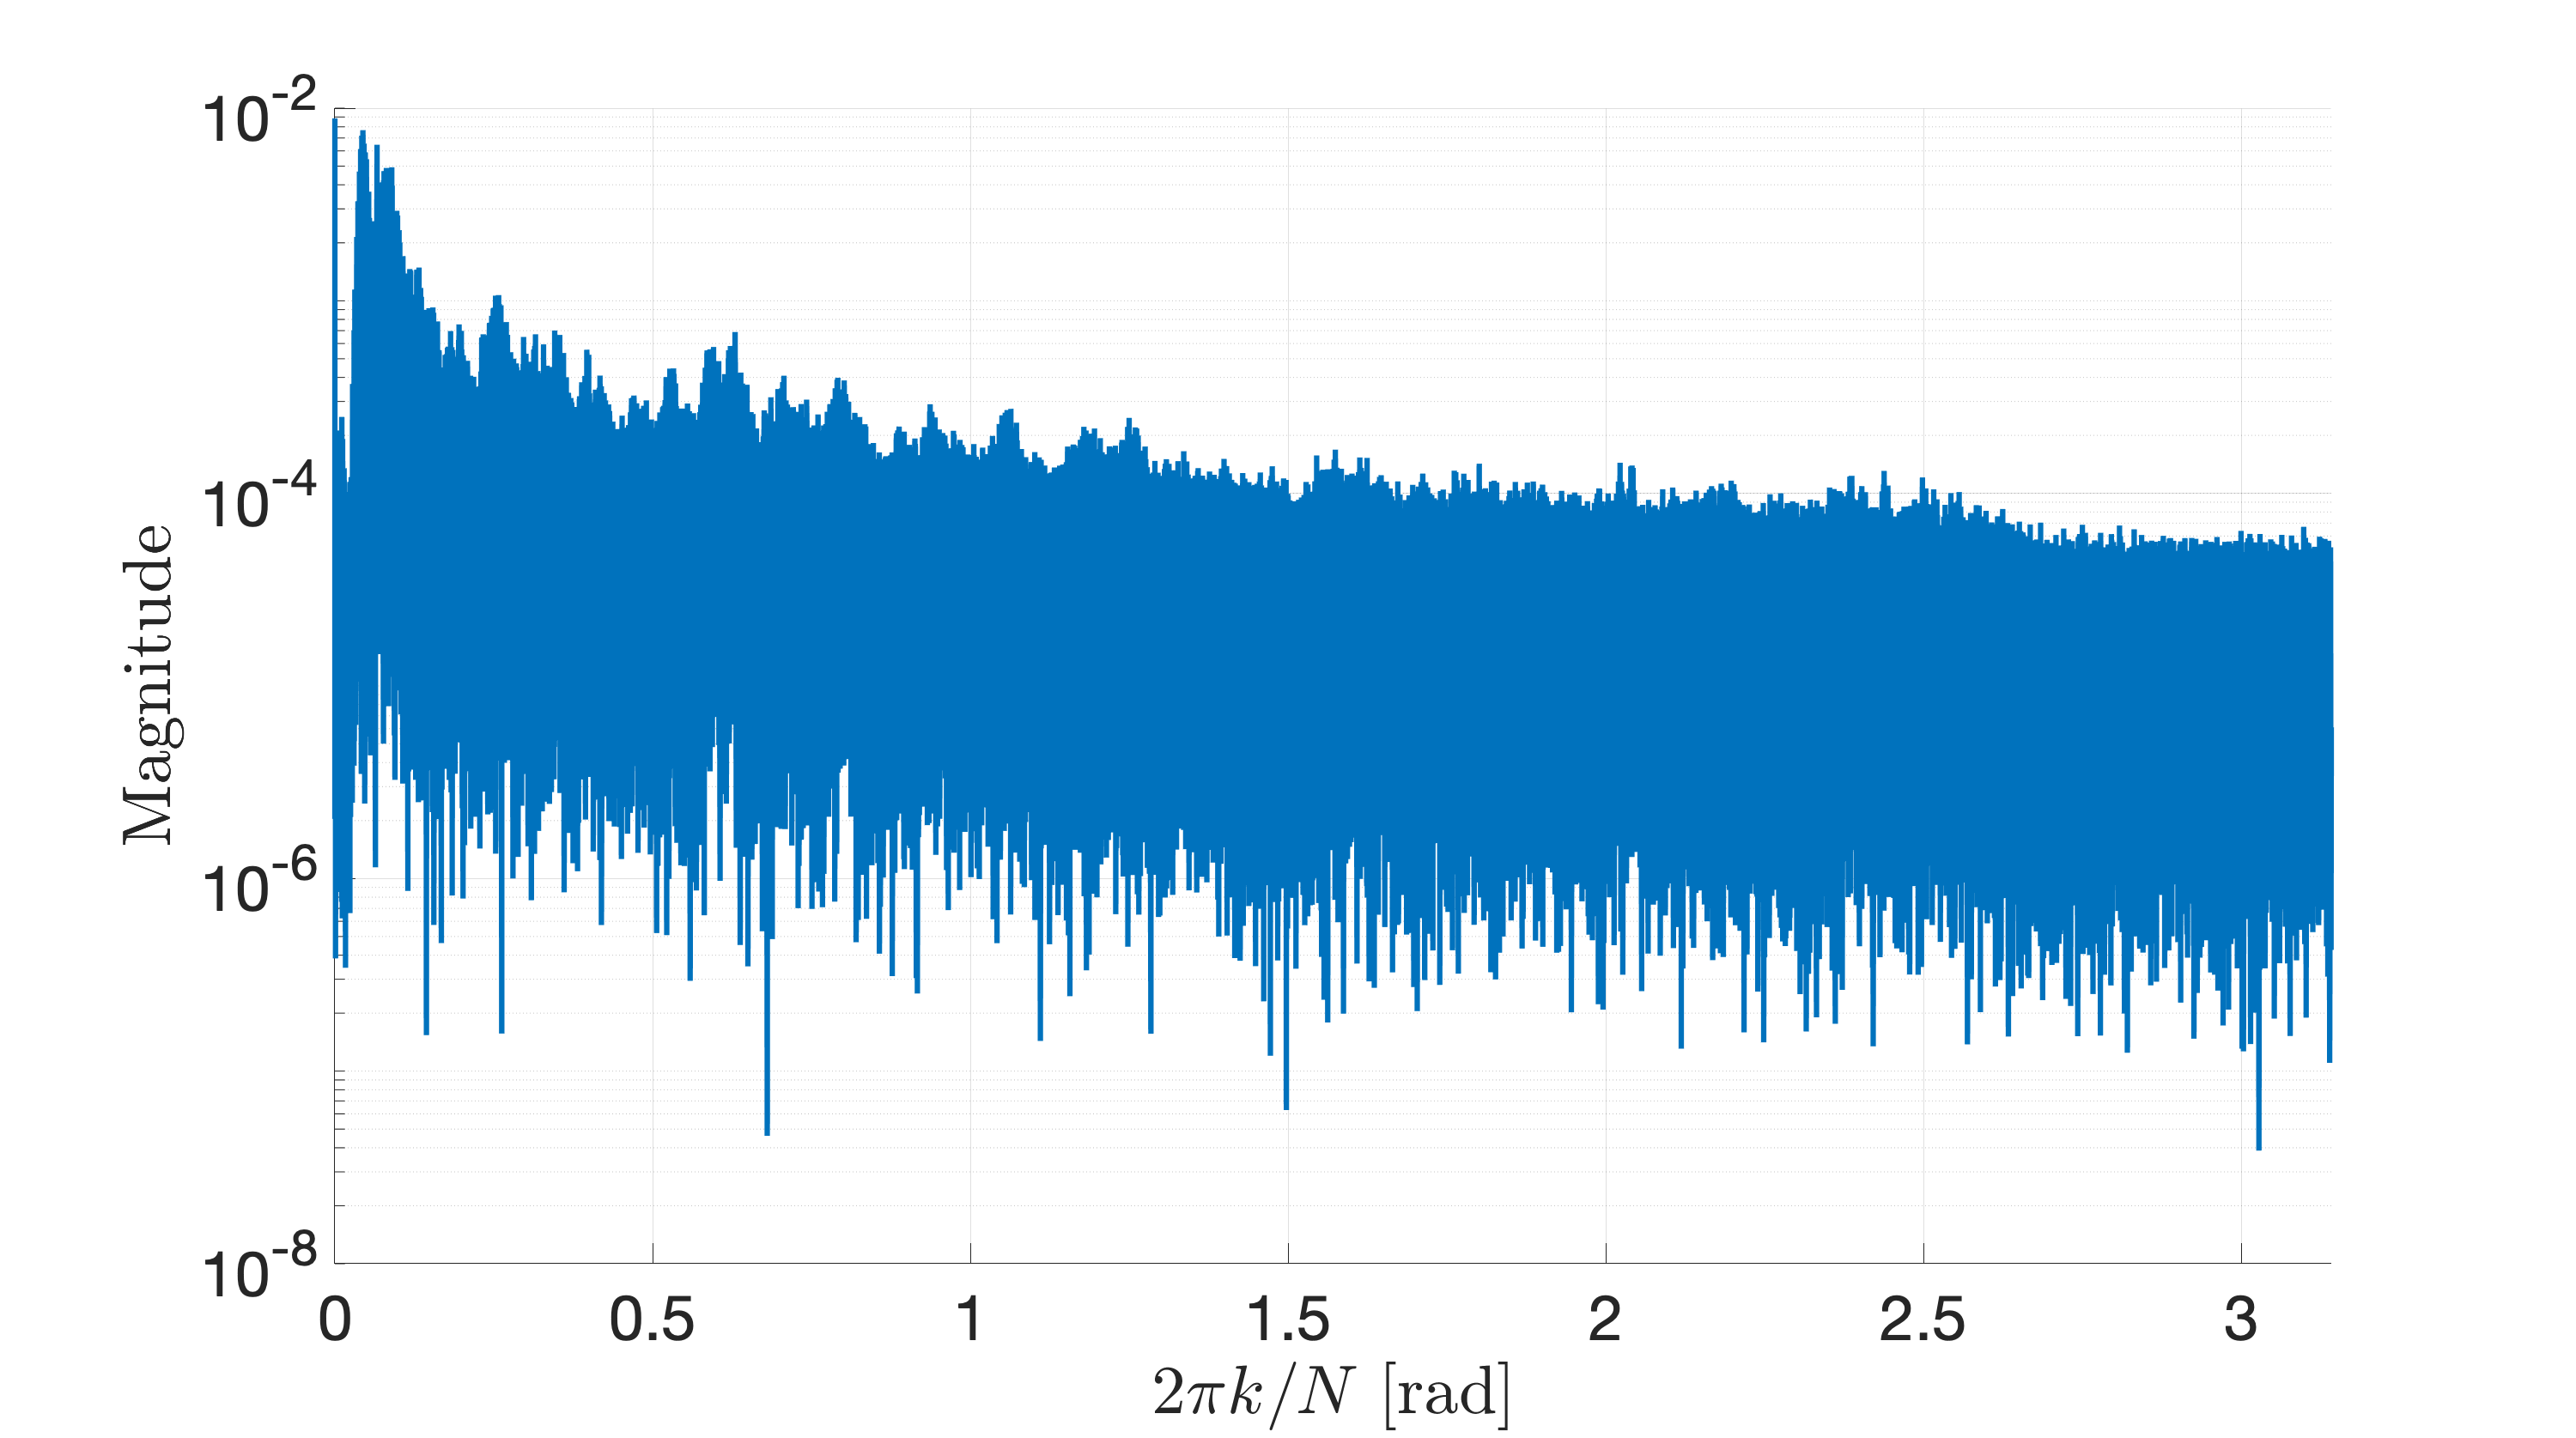
\includegraphics[width= 1.1\textwidth]{figures/R1c.png}
		\caption{Magnitude spectrum of the original sound signal.}
		\label{fig:R1c}
	\end{minipage}
	\hfill
	\begin{minipage}[b]{.49\textwidth}
		\centering
		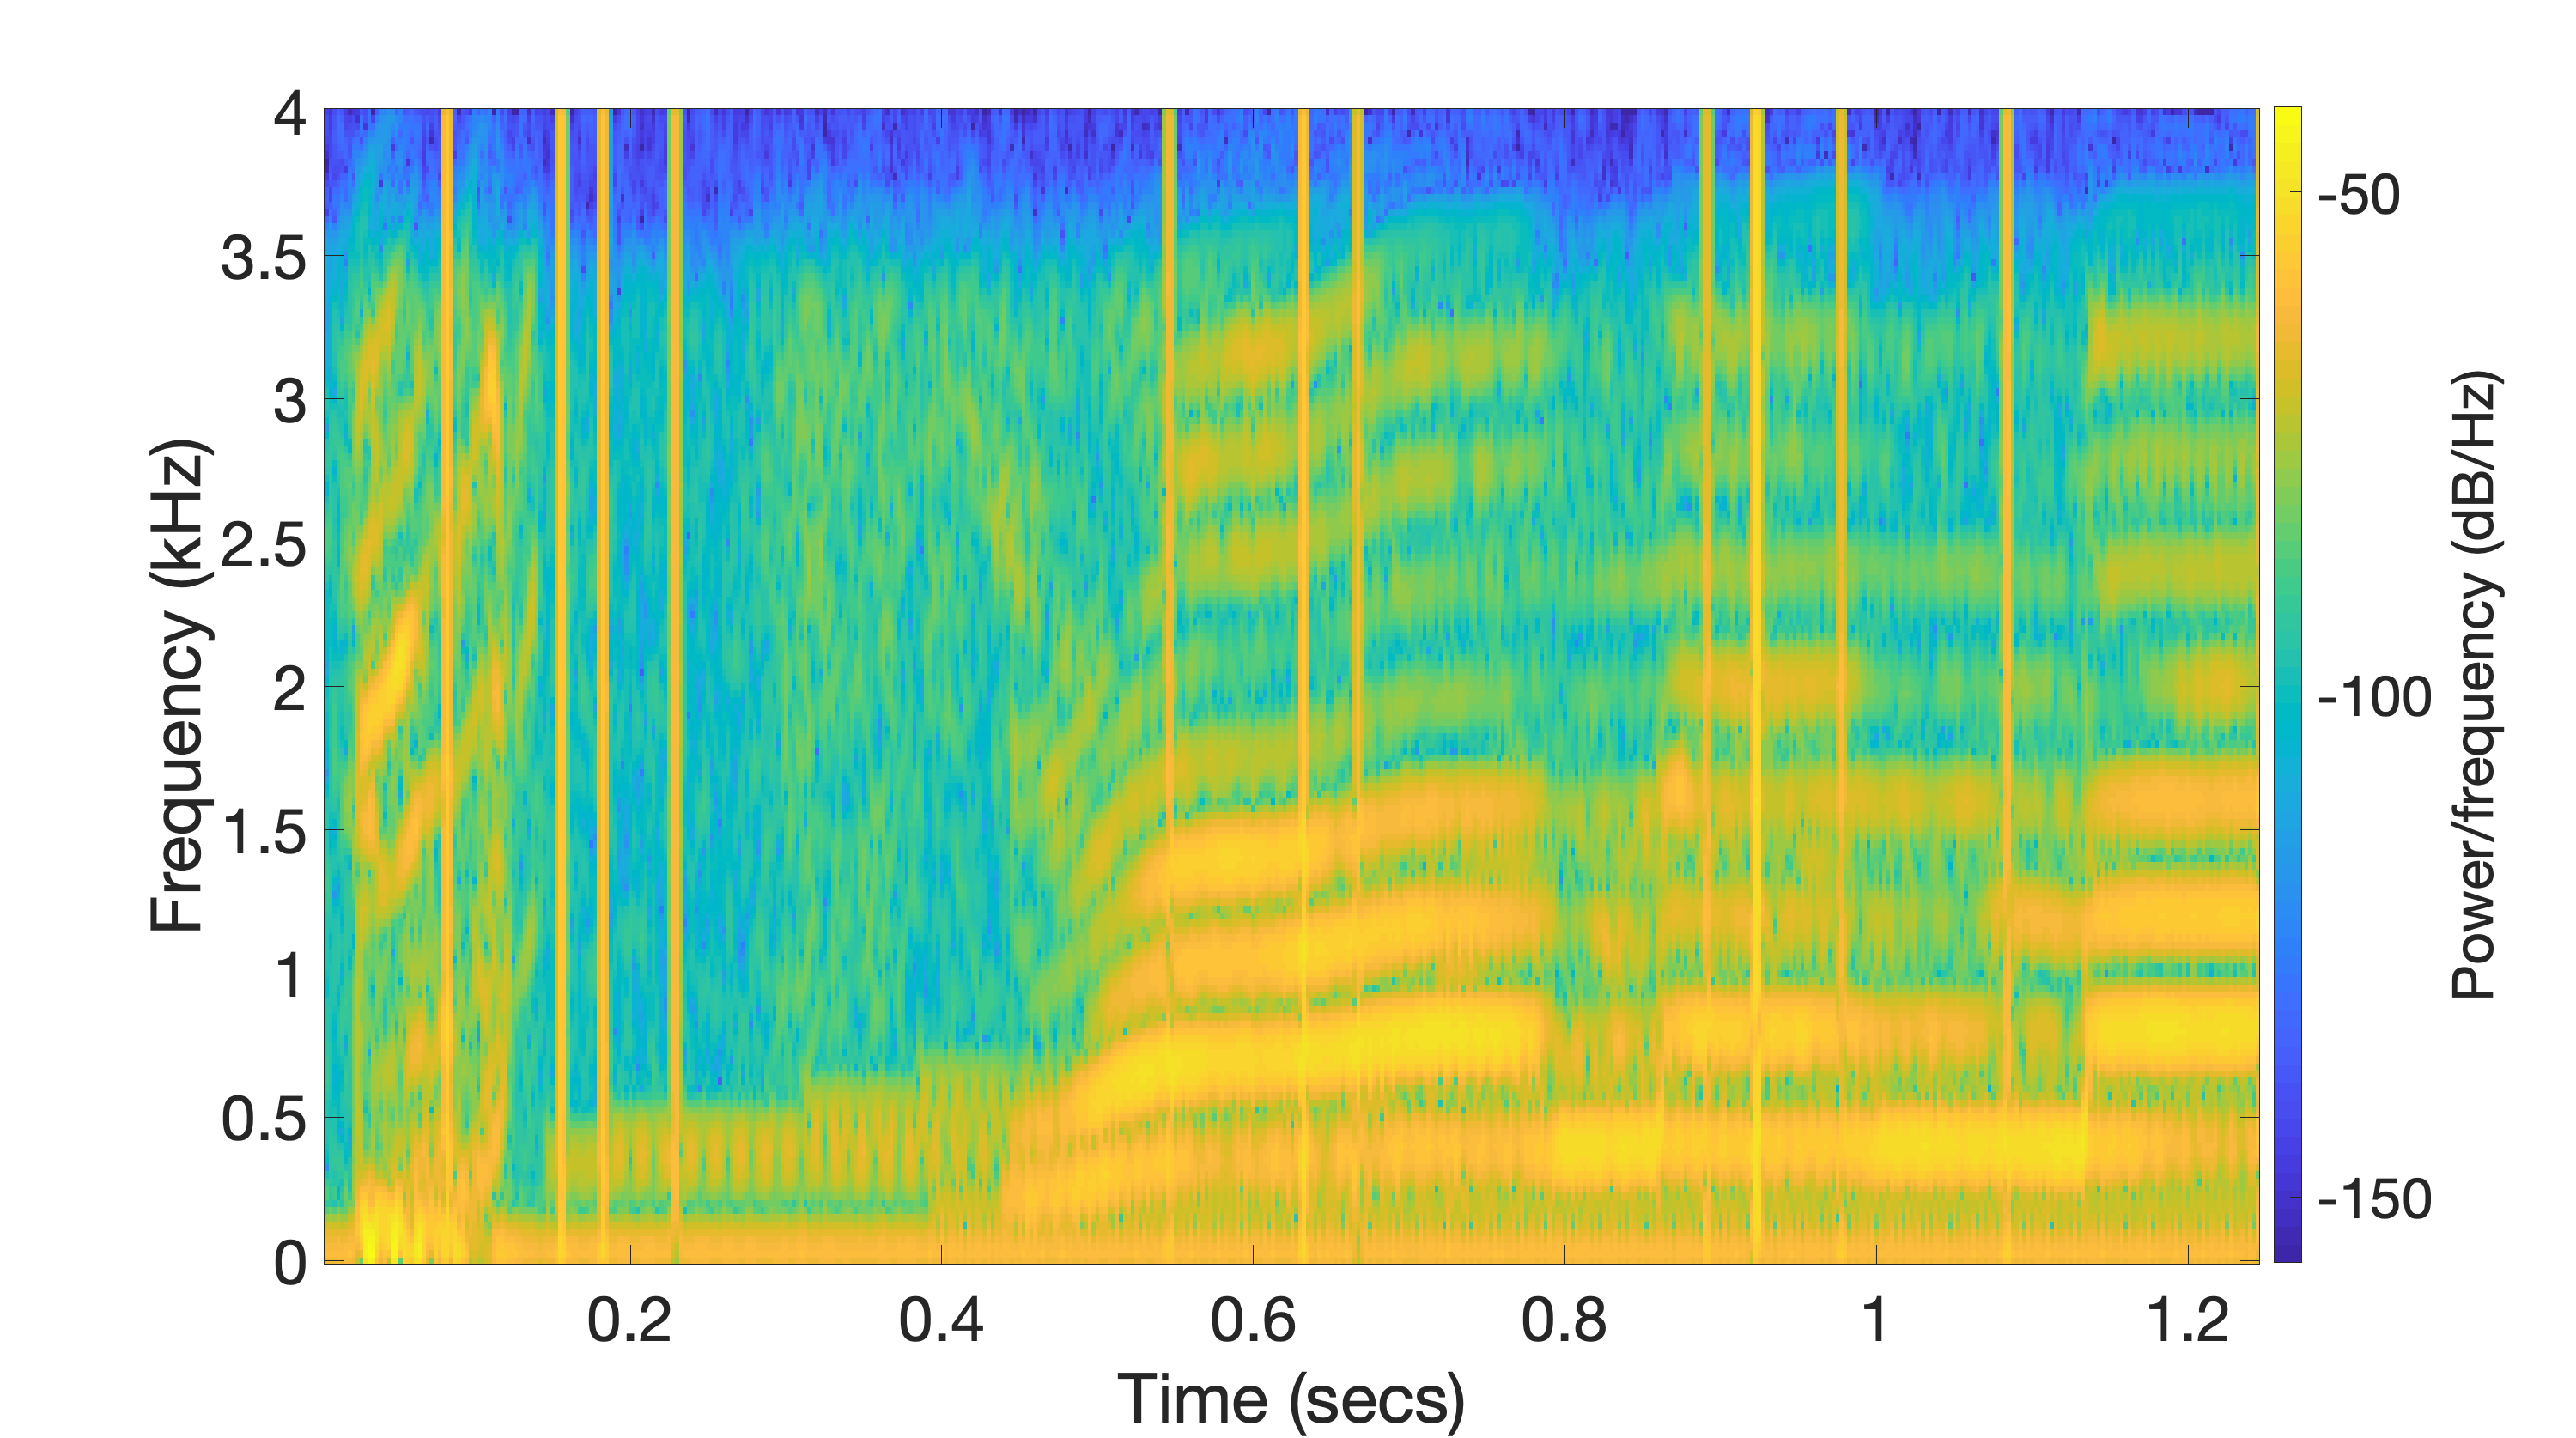
\includegraphics[width= 1.1\textwidth]{figures/R1c_spectrogram.png}
		\caption{Spectrogram.}
		\label{fig:R1c_spectrogram}
	\end{minipage}
\end{figure}

\section{R2. Filtering with an LTI filter}
\subsection{R2.a) Butterworth low-pass filter}
In this and in the following section, two filters are devised to remove the impulsive noise present in the sound signal. First, an LTI Butterworth low-pass filter of order 10 with cutoff frequency $\omega_{co} = \pi/2$ is computed. The magnitude, in linear coordinates, and phase for this filter are shown in Figs. \ref{fig:R2a_gain} and \ref{fig:R2a_phase}, respectively. As it is evident analyzing the gain of the filter, it operates in frequency. The gain is unitary for low frequency and decreases for high frequencies. That is, it attenuates frequencies to the right of the vertical dashed line, which represents the cutoff frequency, and the frequencies to the left are almost not affected by the filter in terms of amplitude.

\begin{figure}[htbp]
	\centering
	\begin{minipage}[b]{.49\textwidth}
		\centering
		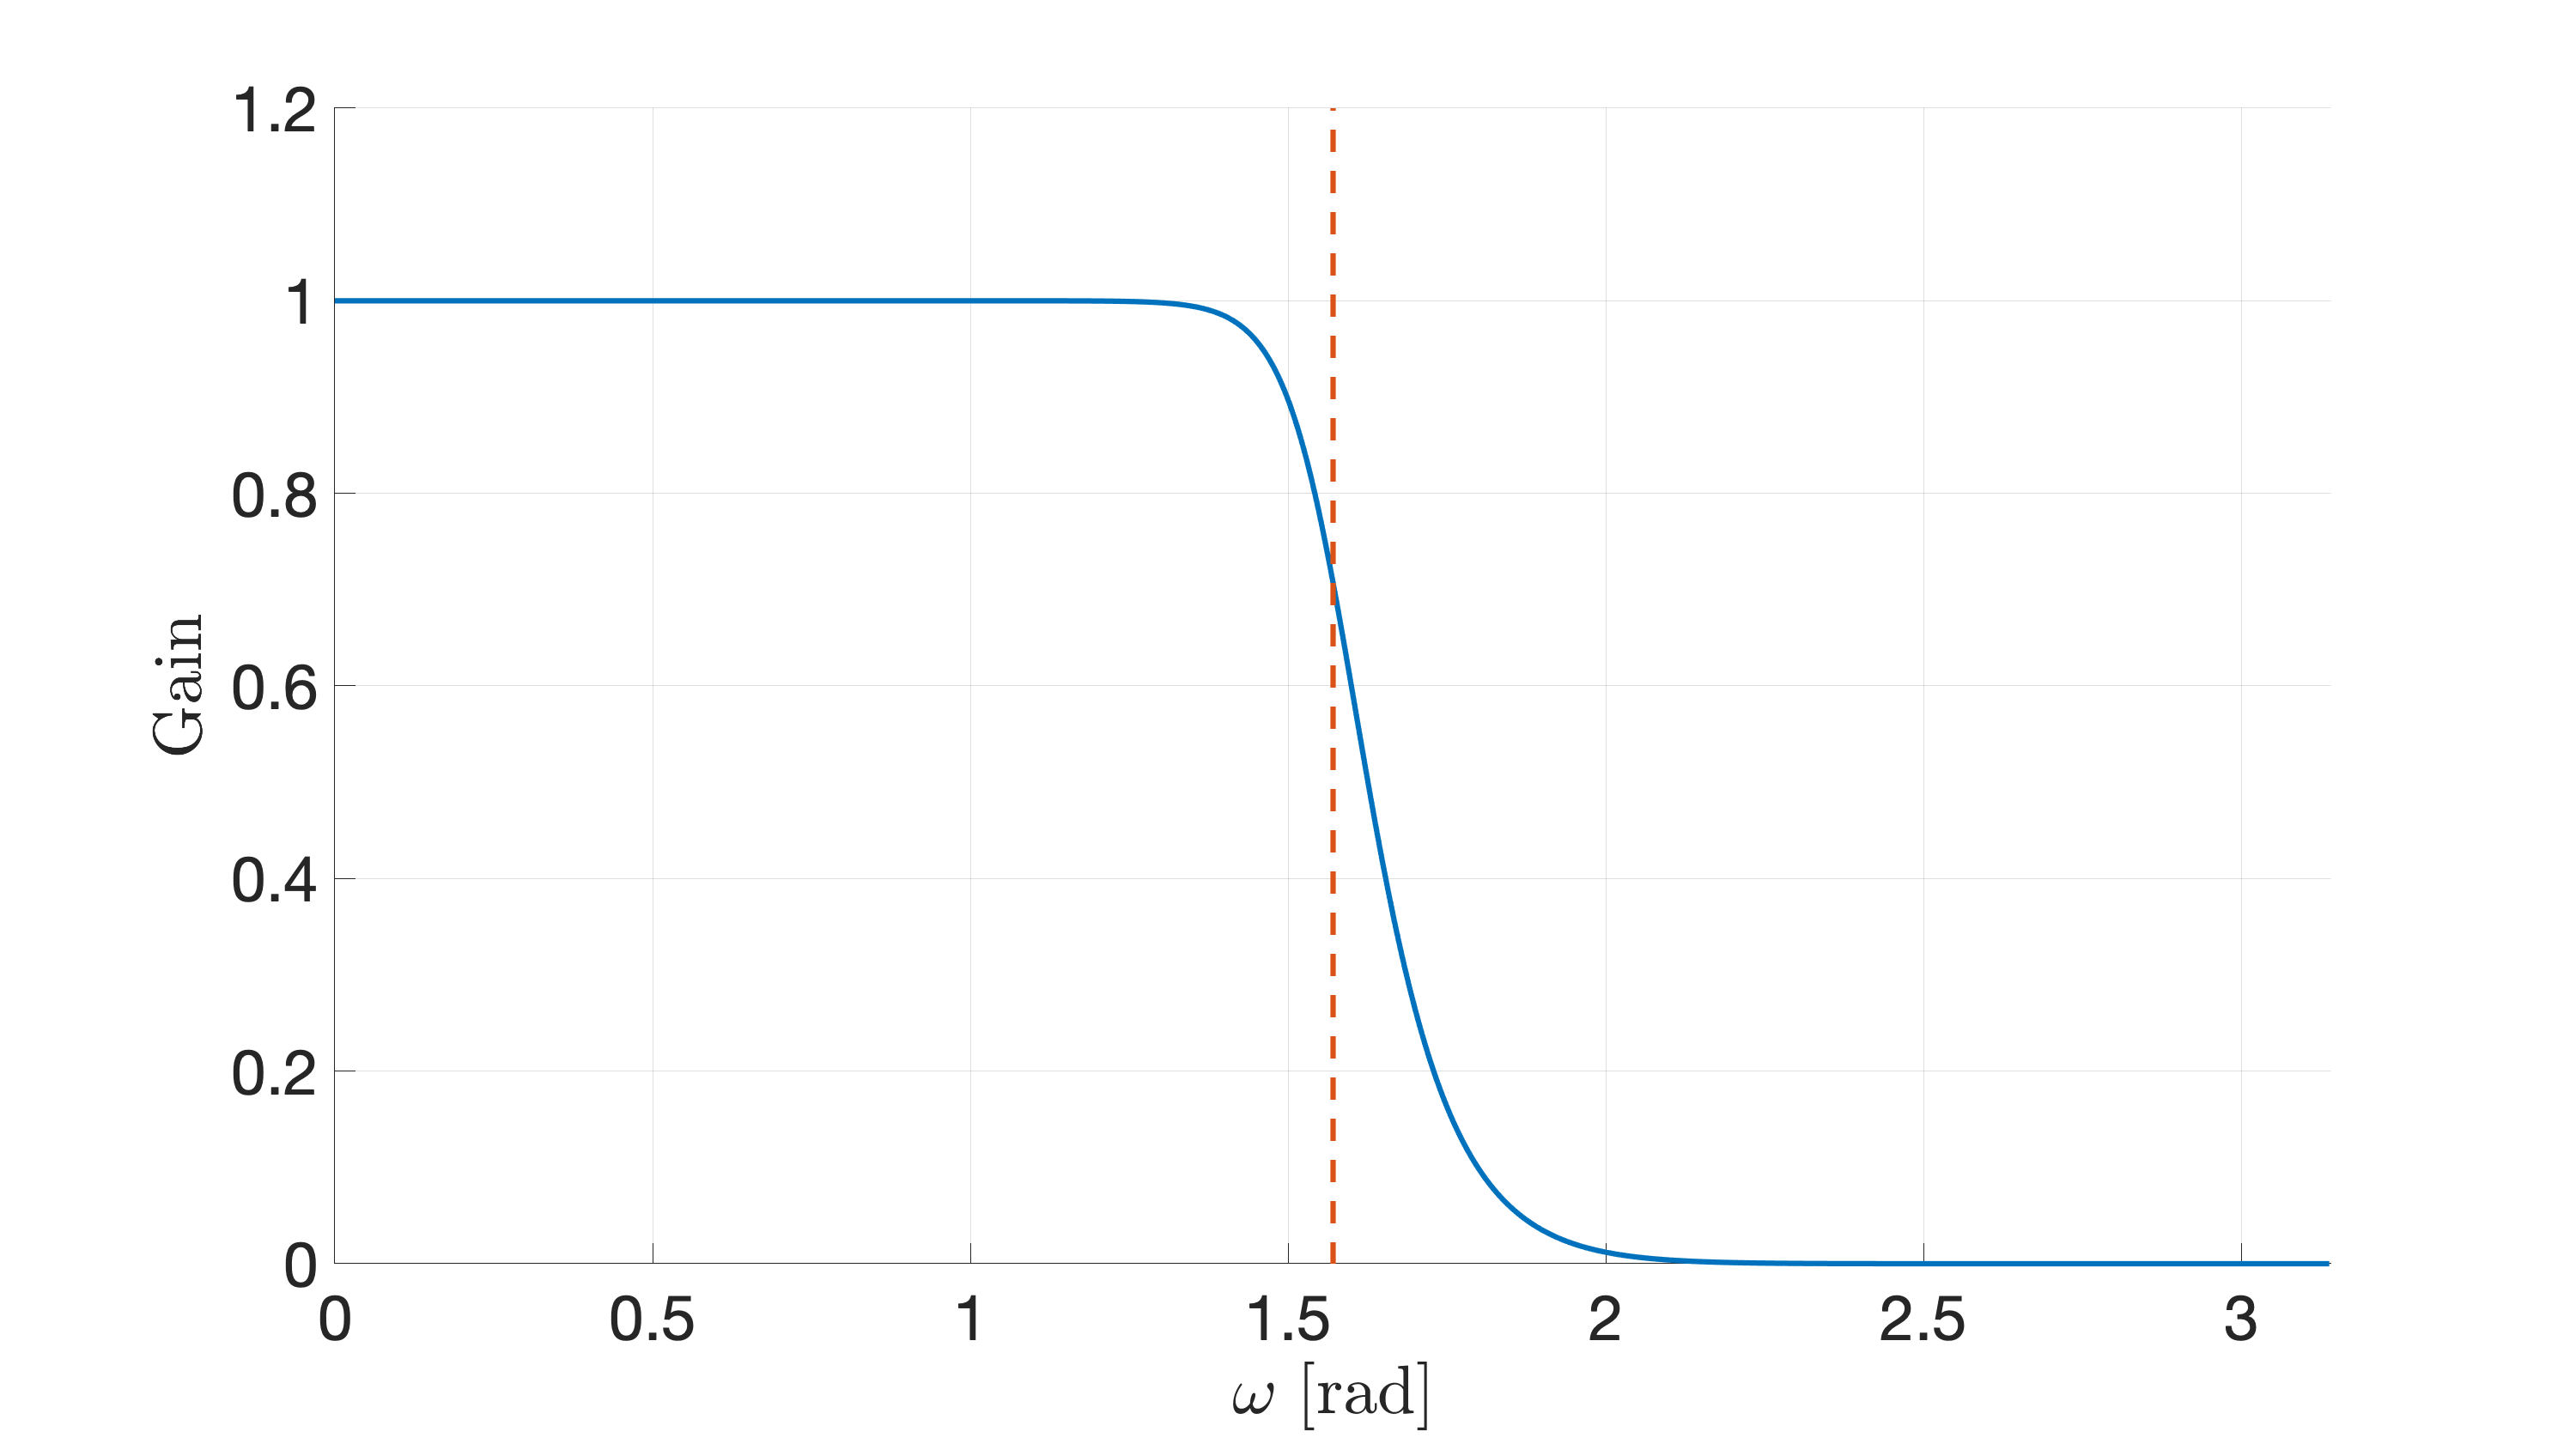
\includegraphics[width= 1.1\textwidth]{figures/R2a_gain.png}
		\caption{Gain in linear coordinates of the LTI filter.}
		\label{fig:R2a_gain}
	\end{minipage}
	\hfill
	\begin{minipage}[b]{.49\textwidth}
		\centering
		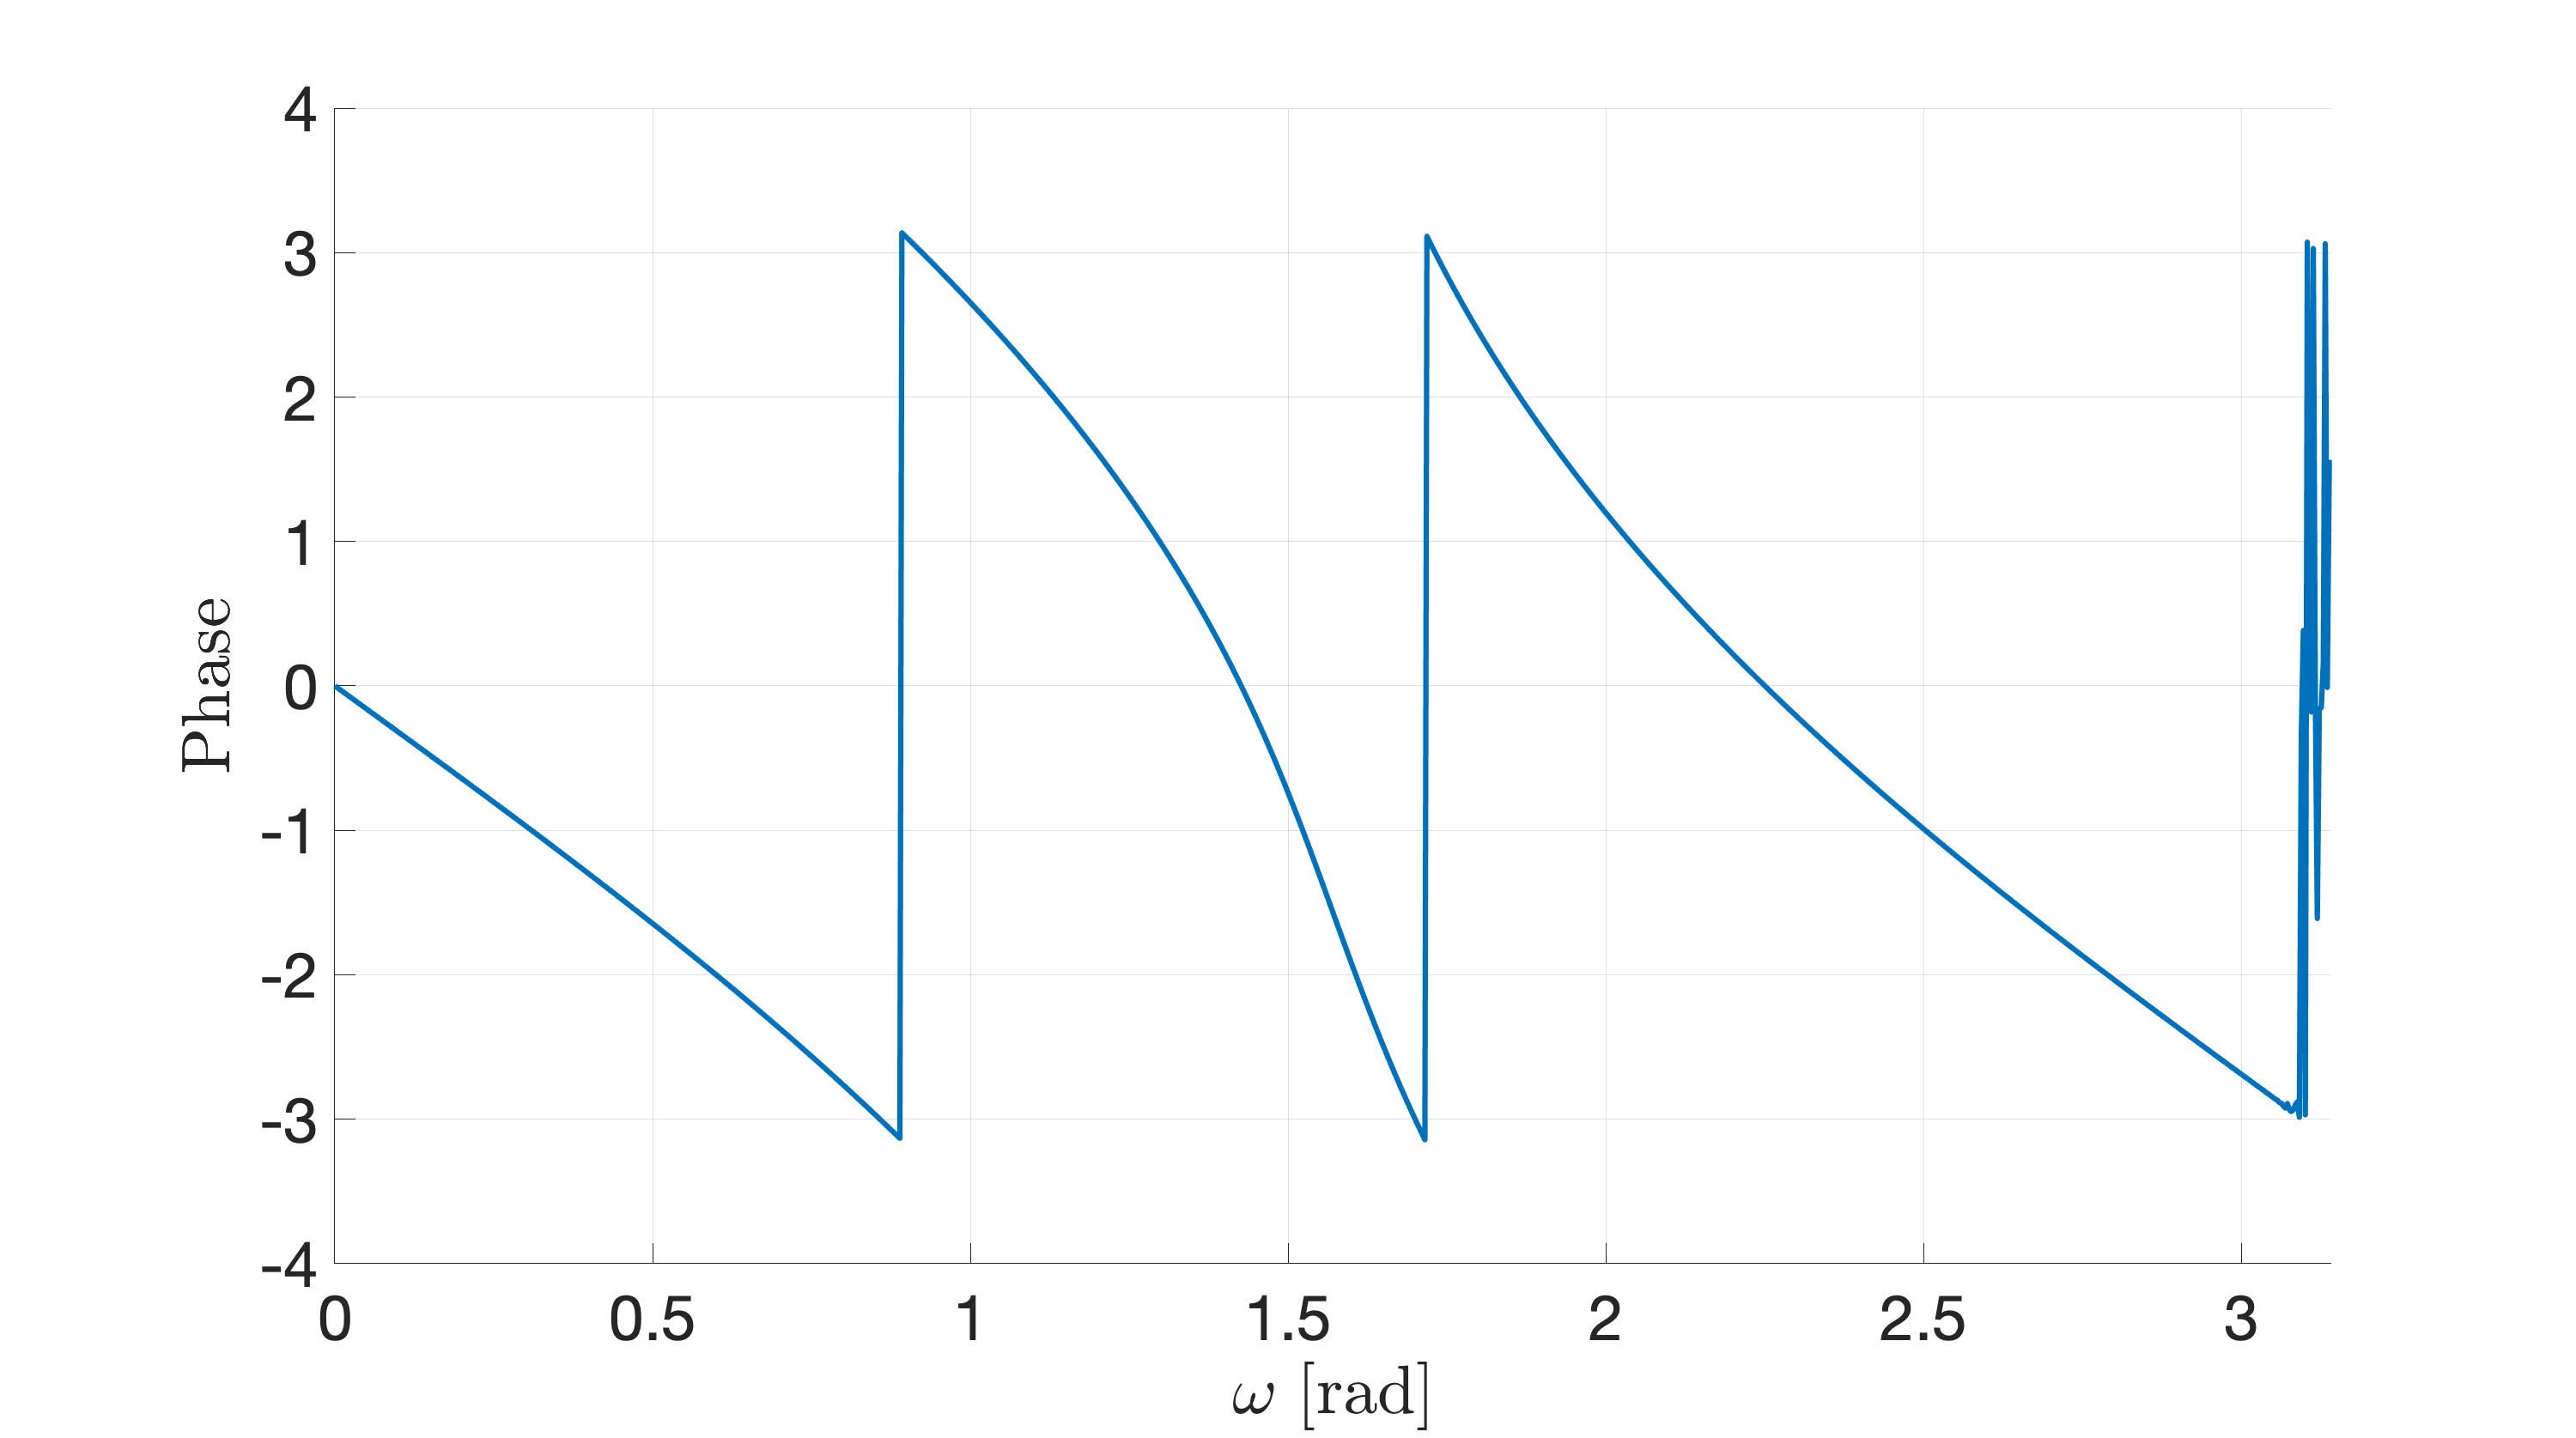
\includegraphics[width= 1.1\textwidth]{figures/R2a_phase.png}
		\caption{Phase of the LTI filter.}
		\label{fig:R2a_phase}
	\end{minipage}
\end{figure}

\subsection{R2.b) Filtered signal}
The continuous time cutoff frequency can be obtained by the following relation
\begin{equation*}
\Omega = \omega/T \iff f_{co} = \frac{\omega_{co}}{2\pi}f_s = 2 \text{kHz}\:,
\end{equation*}
where $T$ and $f_s$ are, respectively, the sampling period and the sampling frequency.

\subsection{R2.c) Analysis of the filtered signal in the time domain}

Figs. \ref{fig:R2c}--\ref{fig:R2c_zoomNormal} show the comparison of the filtered signal and the original signal in the time domain for various segments of the song. First, it is seen in Fig. \ref{fig:R2c} that although the noise impulses are attenuated in relation to the original signal, they are still very significant. This is expected, since in the frequency domain the impulses are represented by a constant and this filter is attenuating only the portion that is in the higher frequencies. Although the segments of the signal which are not corrupted by noise are attenuated, this attenuation is not significant. Second, Fig. \ref{fig:R2c} shows a zoom of the signal, where it is possible to see the effect of the distortion caused by the filter. Third, in Fig. \ref{fig:R2c_zoomNoise} it is possible to analyze more closely the behavior of the filter after a noise impulse in the time domain. After the noise impulse, as expected, the response of the noiseless signal is superimposed with the impulse response of the filter, which is an IIR. The impulse response of the filter is oscillatory and similar to the response of an under-damped second order system. Fourth, in Fig. \ref{fig:R2c_zoomNormal} it is possible to notice the delay introduced by the filter. Furthermore, given that the phase of the filter, represented in \ref{fig:R2a_phase}, is not linear, then the delay of the filter varies with frequency, which is also a source of distortion.

\begin{figure}[htbp]
	\centering
	\begin{minipage}[b]{.49\textwidth}
		\centering
		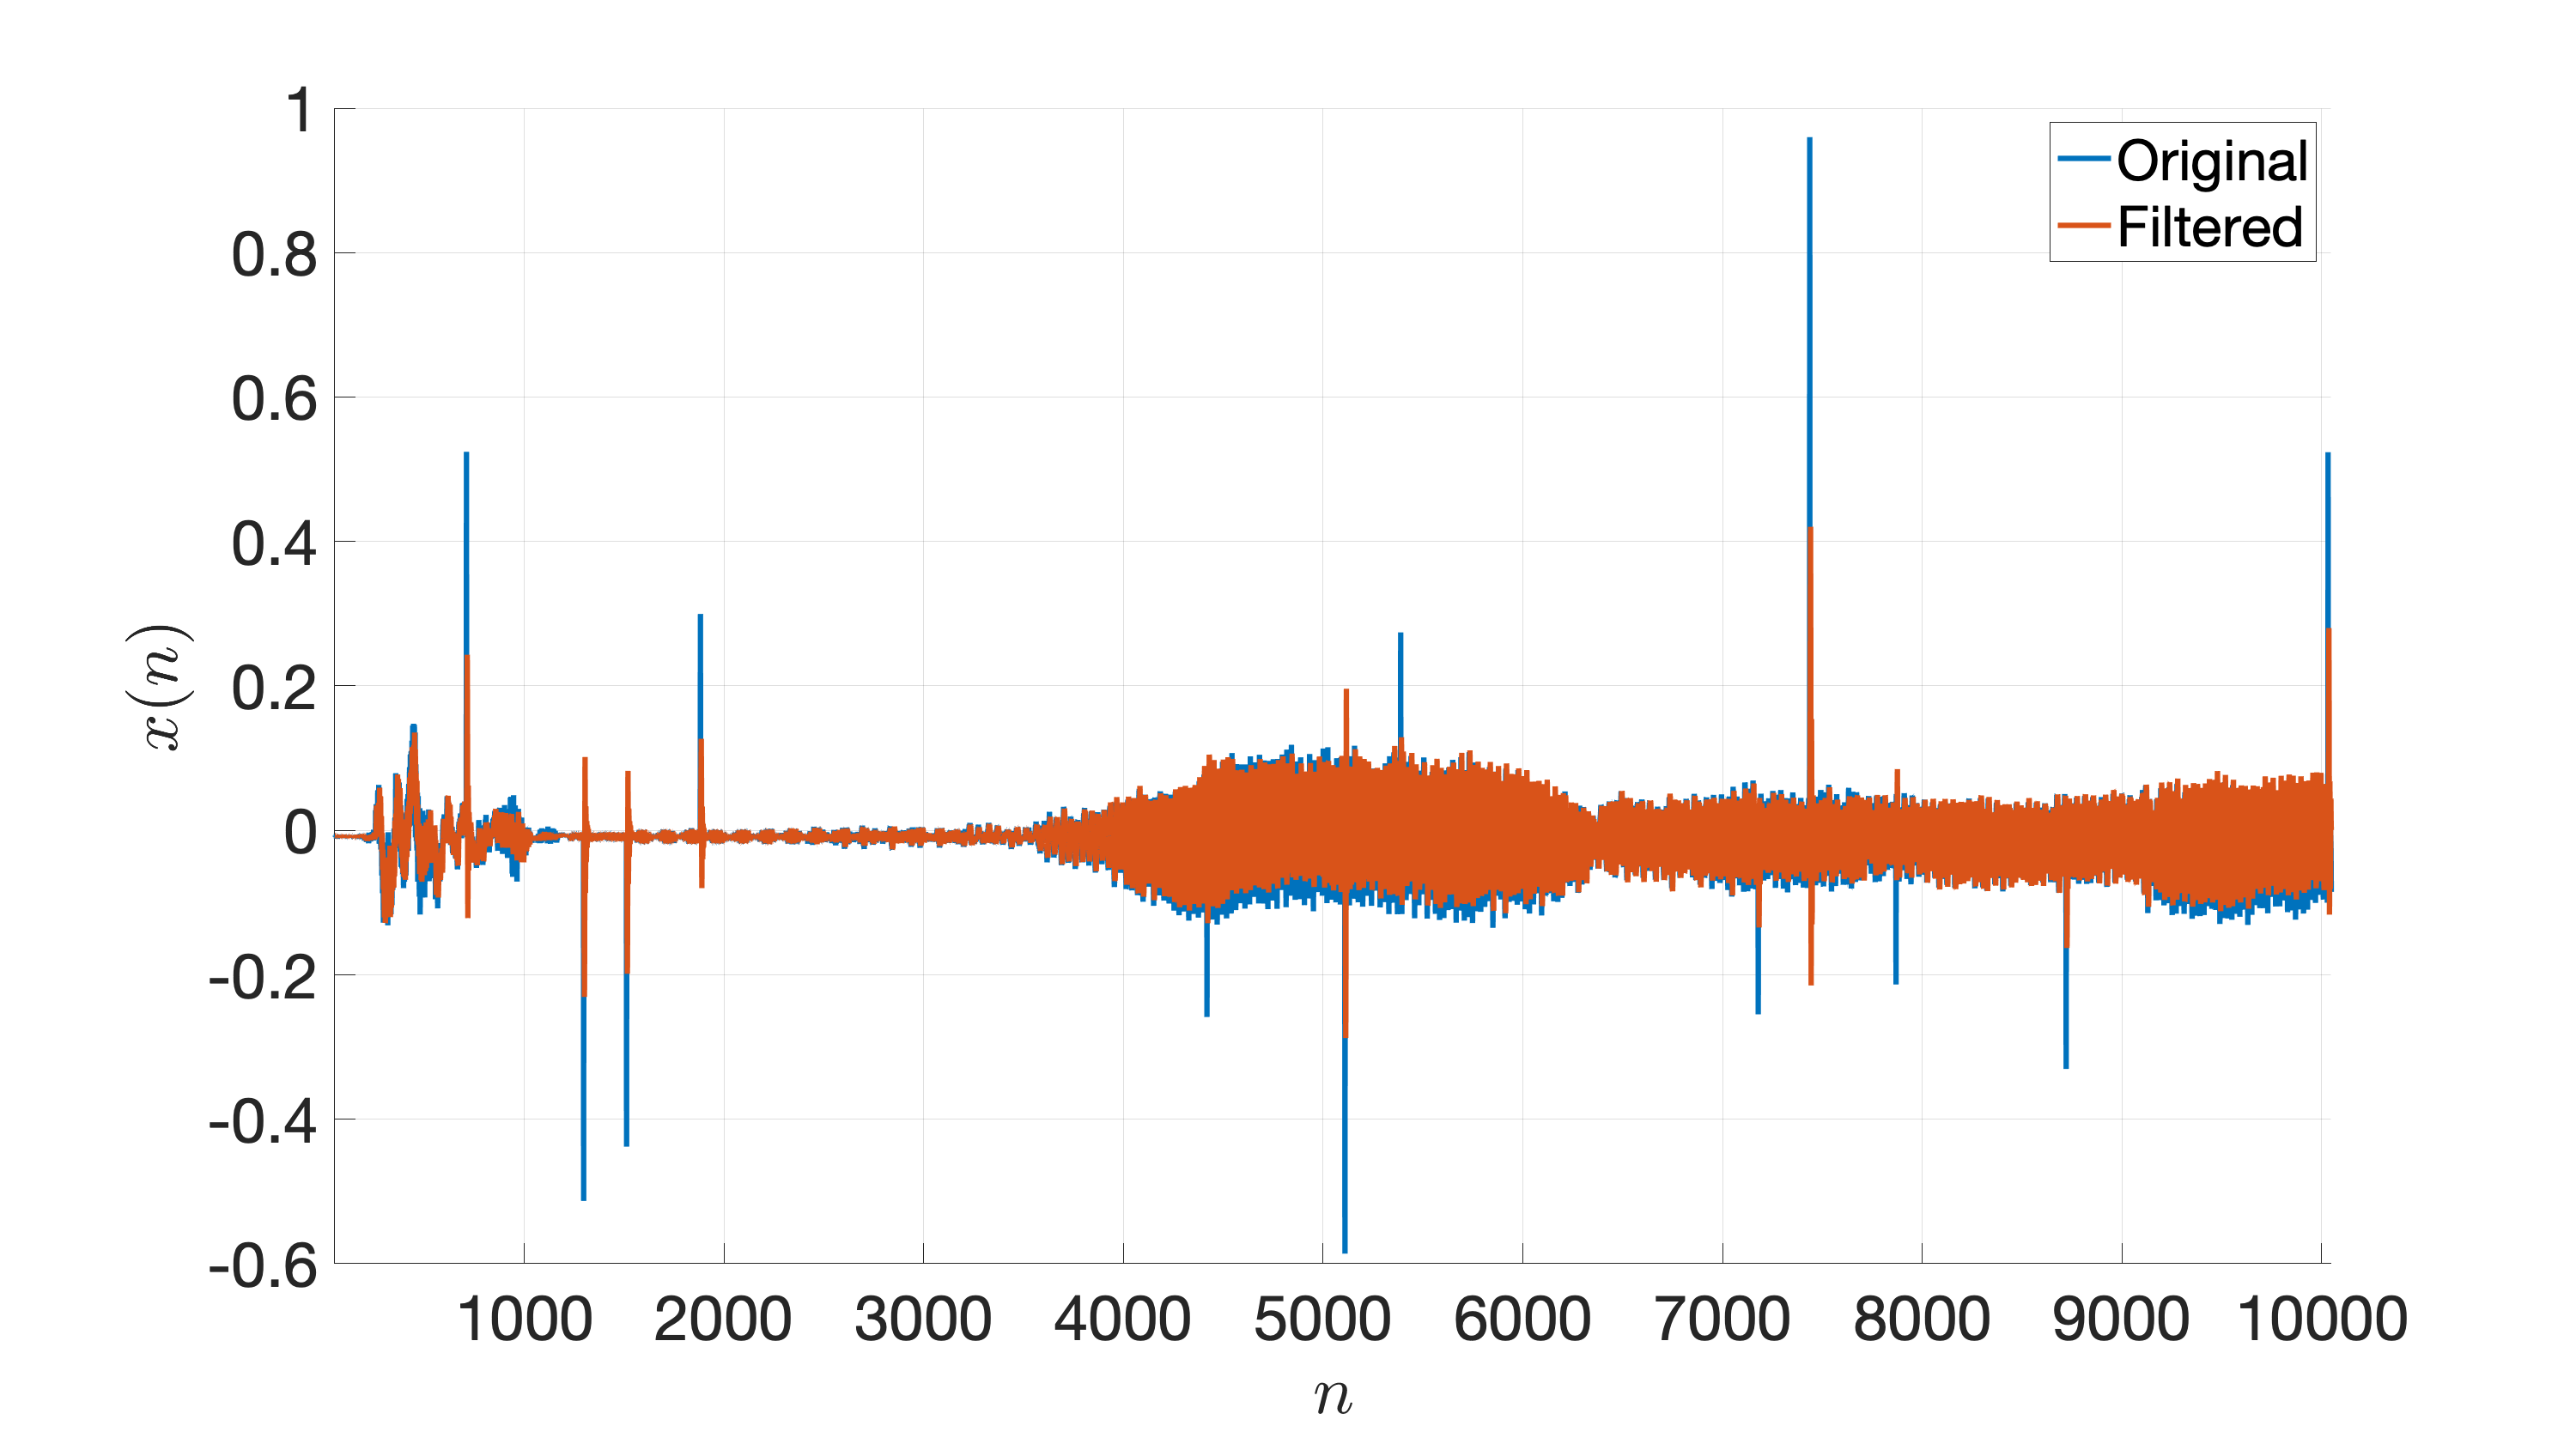
\includegraphics[width= 1.1\textwidth]{figures/R2c.png}
		\caption{LTI filtered signal with $\omega_{co} = \pi/2$.}
		\label{fig:R2c}
	\end{minipage}
	\hfill
	\begin{minipage}[b]{.49\textwidth}
		\centering
		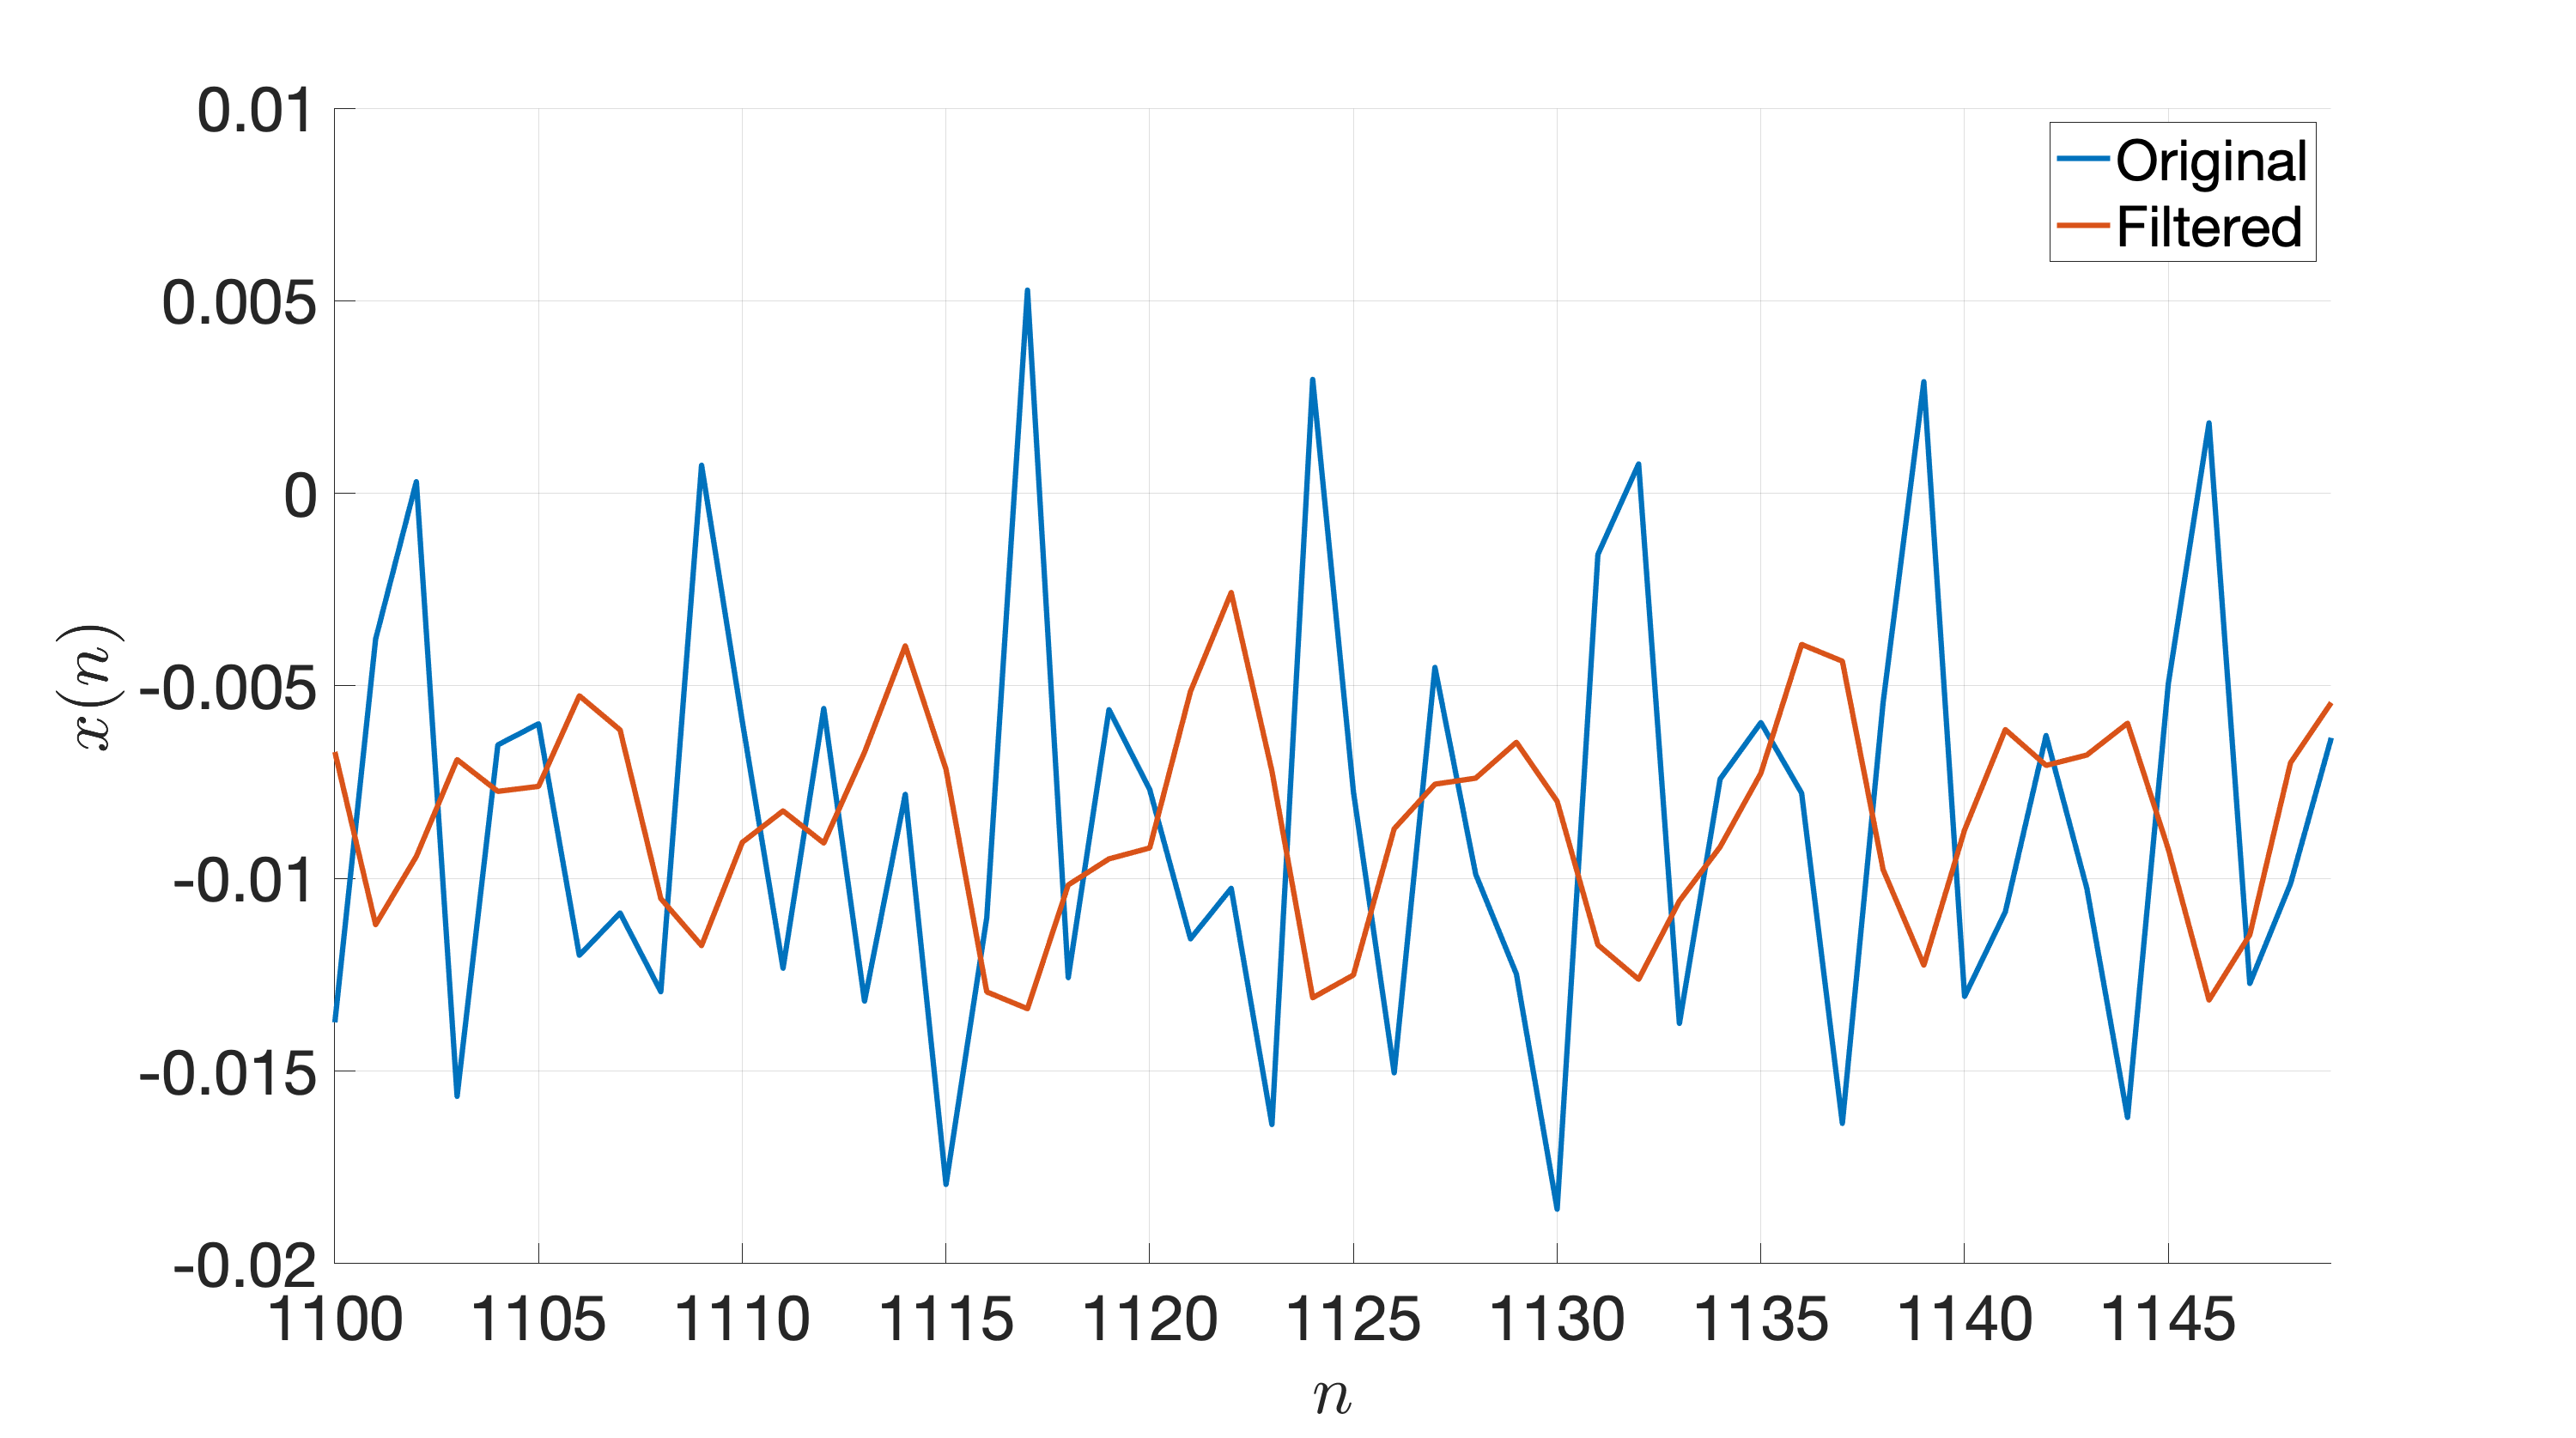
\includegraphics[width= 1.1\textwidth]{figures/R2c_smallAmp.png}
		\caption{LTI filtered signal with $\omega_{co} = \pi/2$.}
		\label{fig:R2c_smallAmp}
	\end{minipage}
\begin{minipage}[b]{.49\textwidth}
	\centering
	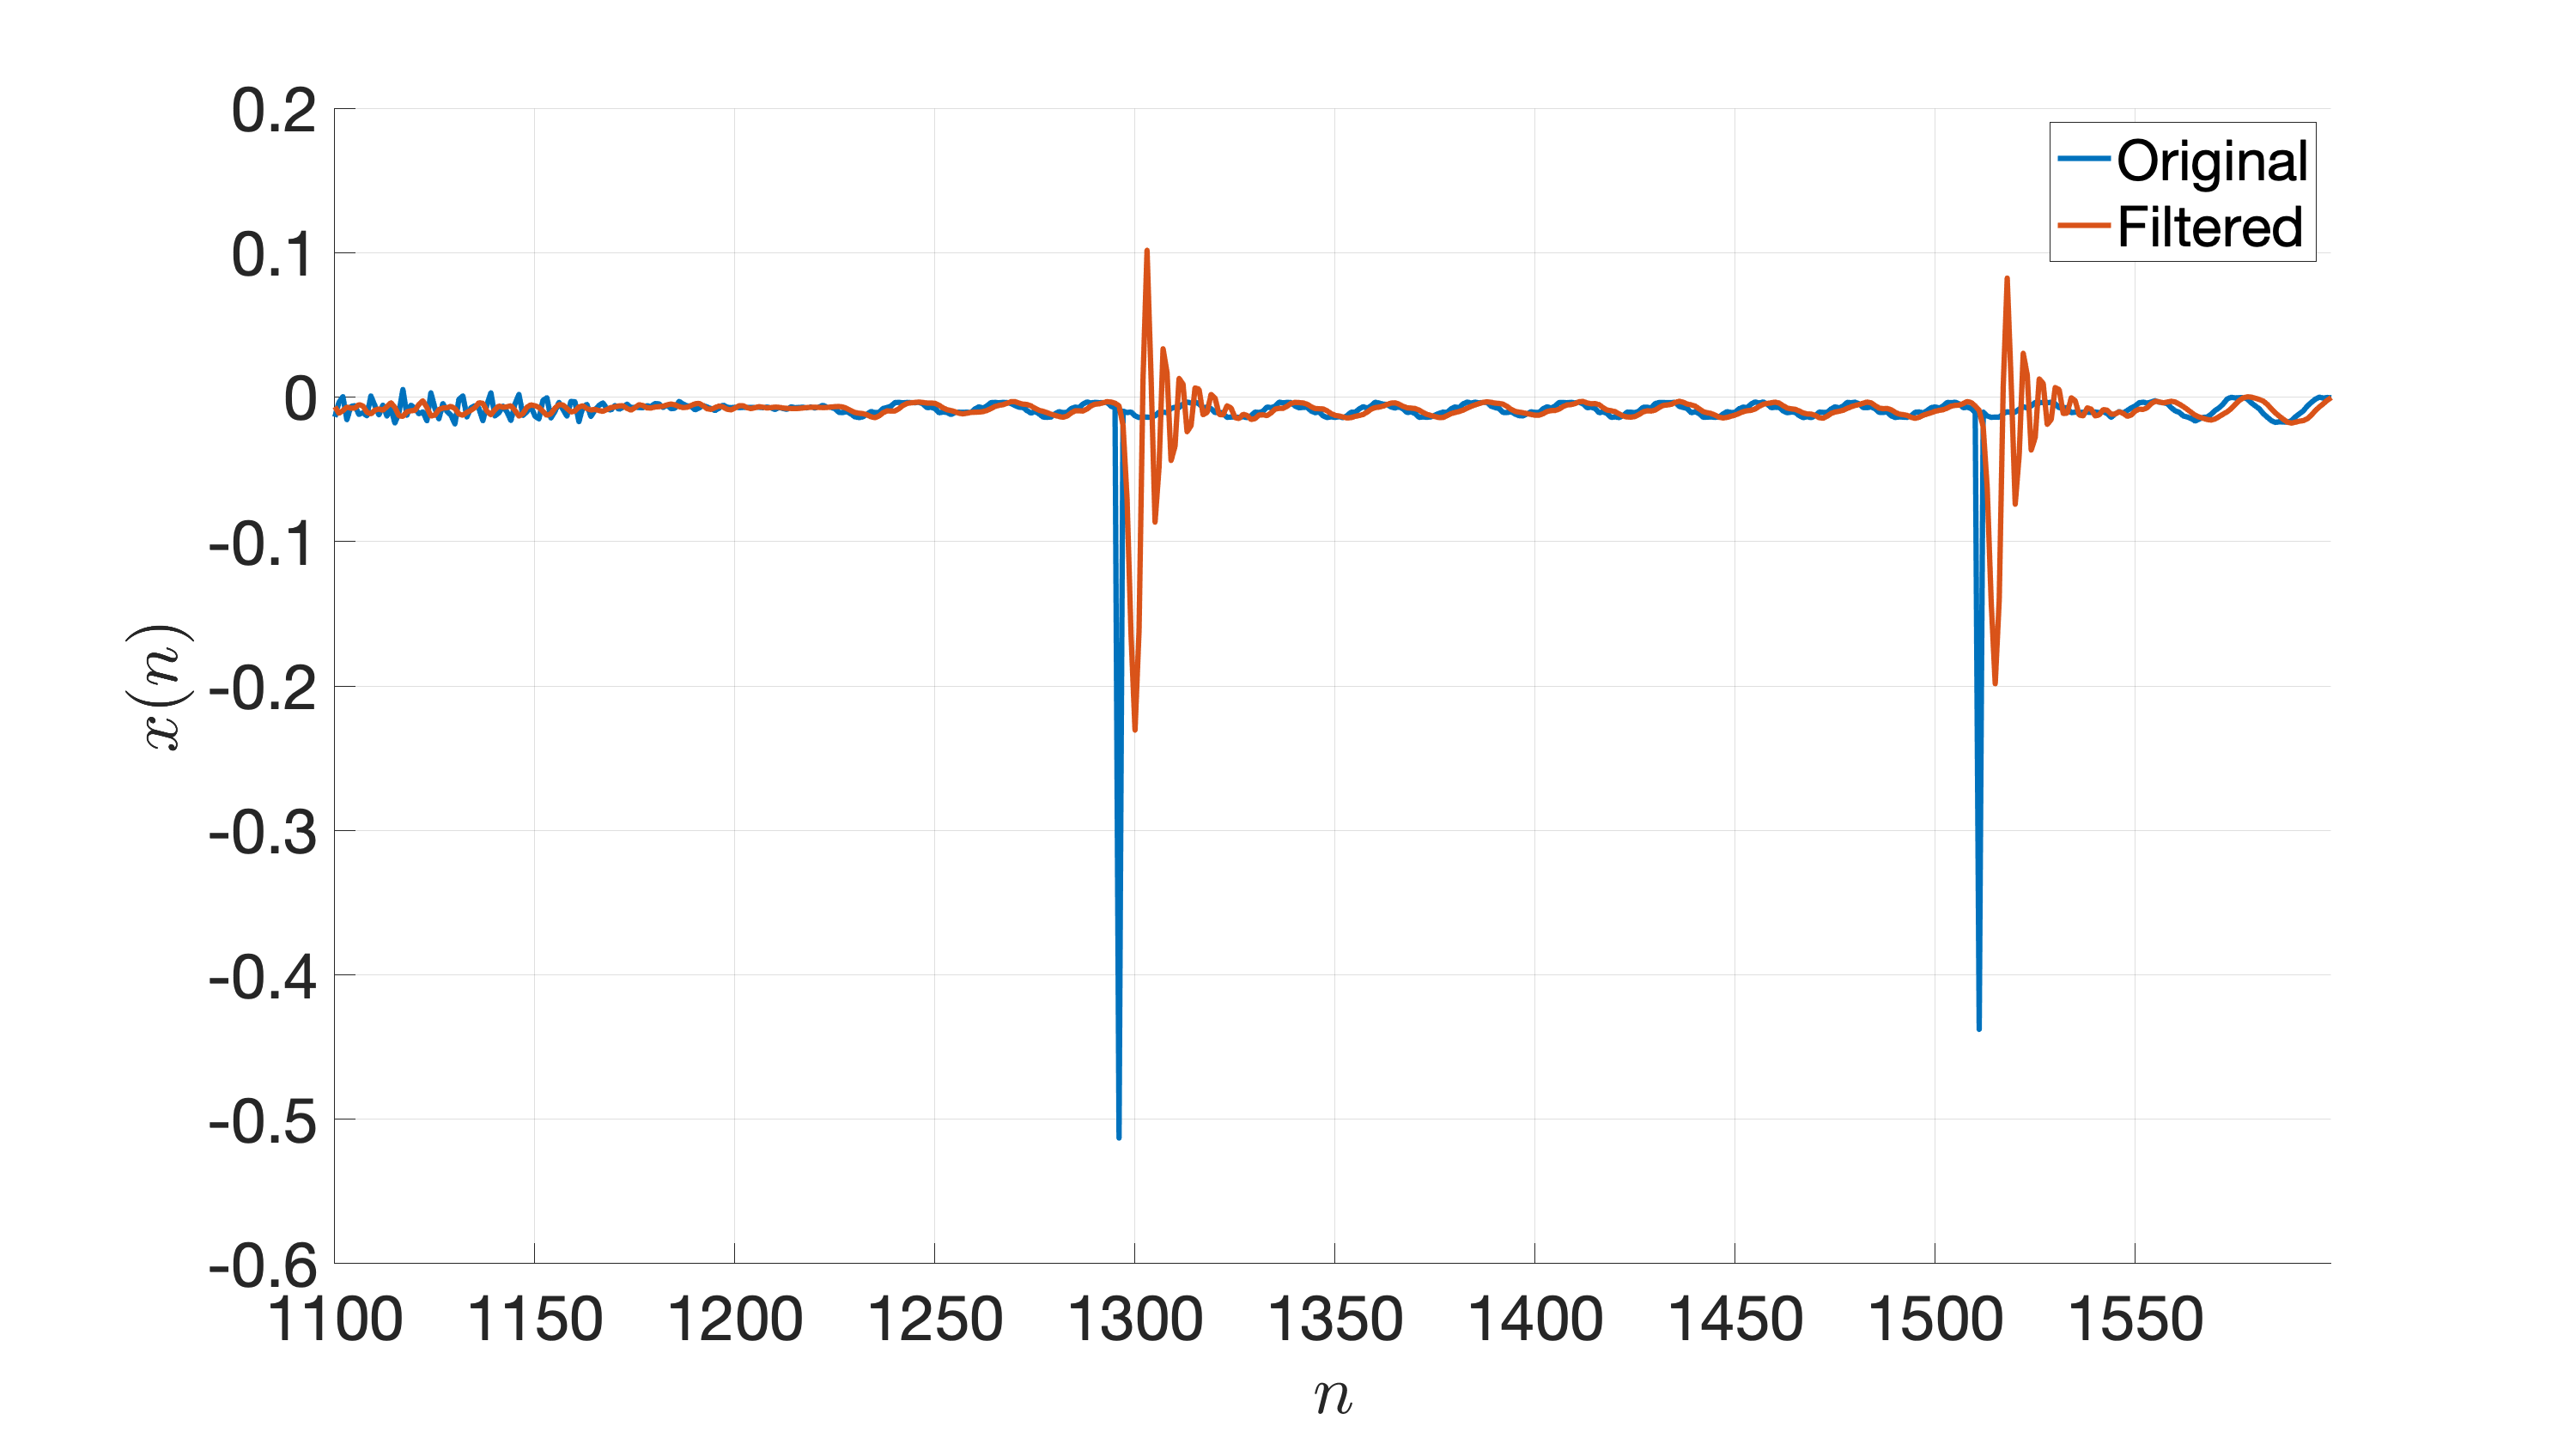
\includegraphics[width= 1.1\textwidth]{figures/R2c_zoomNoise.png}
	\caption{LTI filtered signal with $\omega_{co} = \pi/2$.}
	\label{fig:R2c_zoomNoise}
\end{minipage}
\hfill
\begin{minipage}[b]{.49\textwidth}
	\centering
	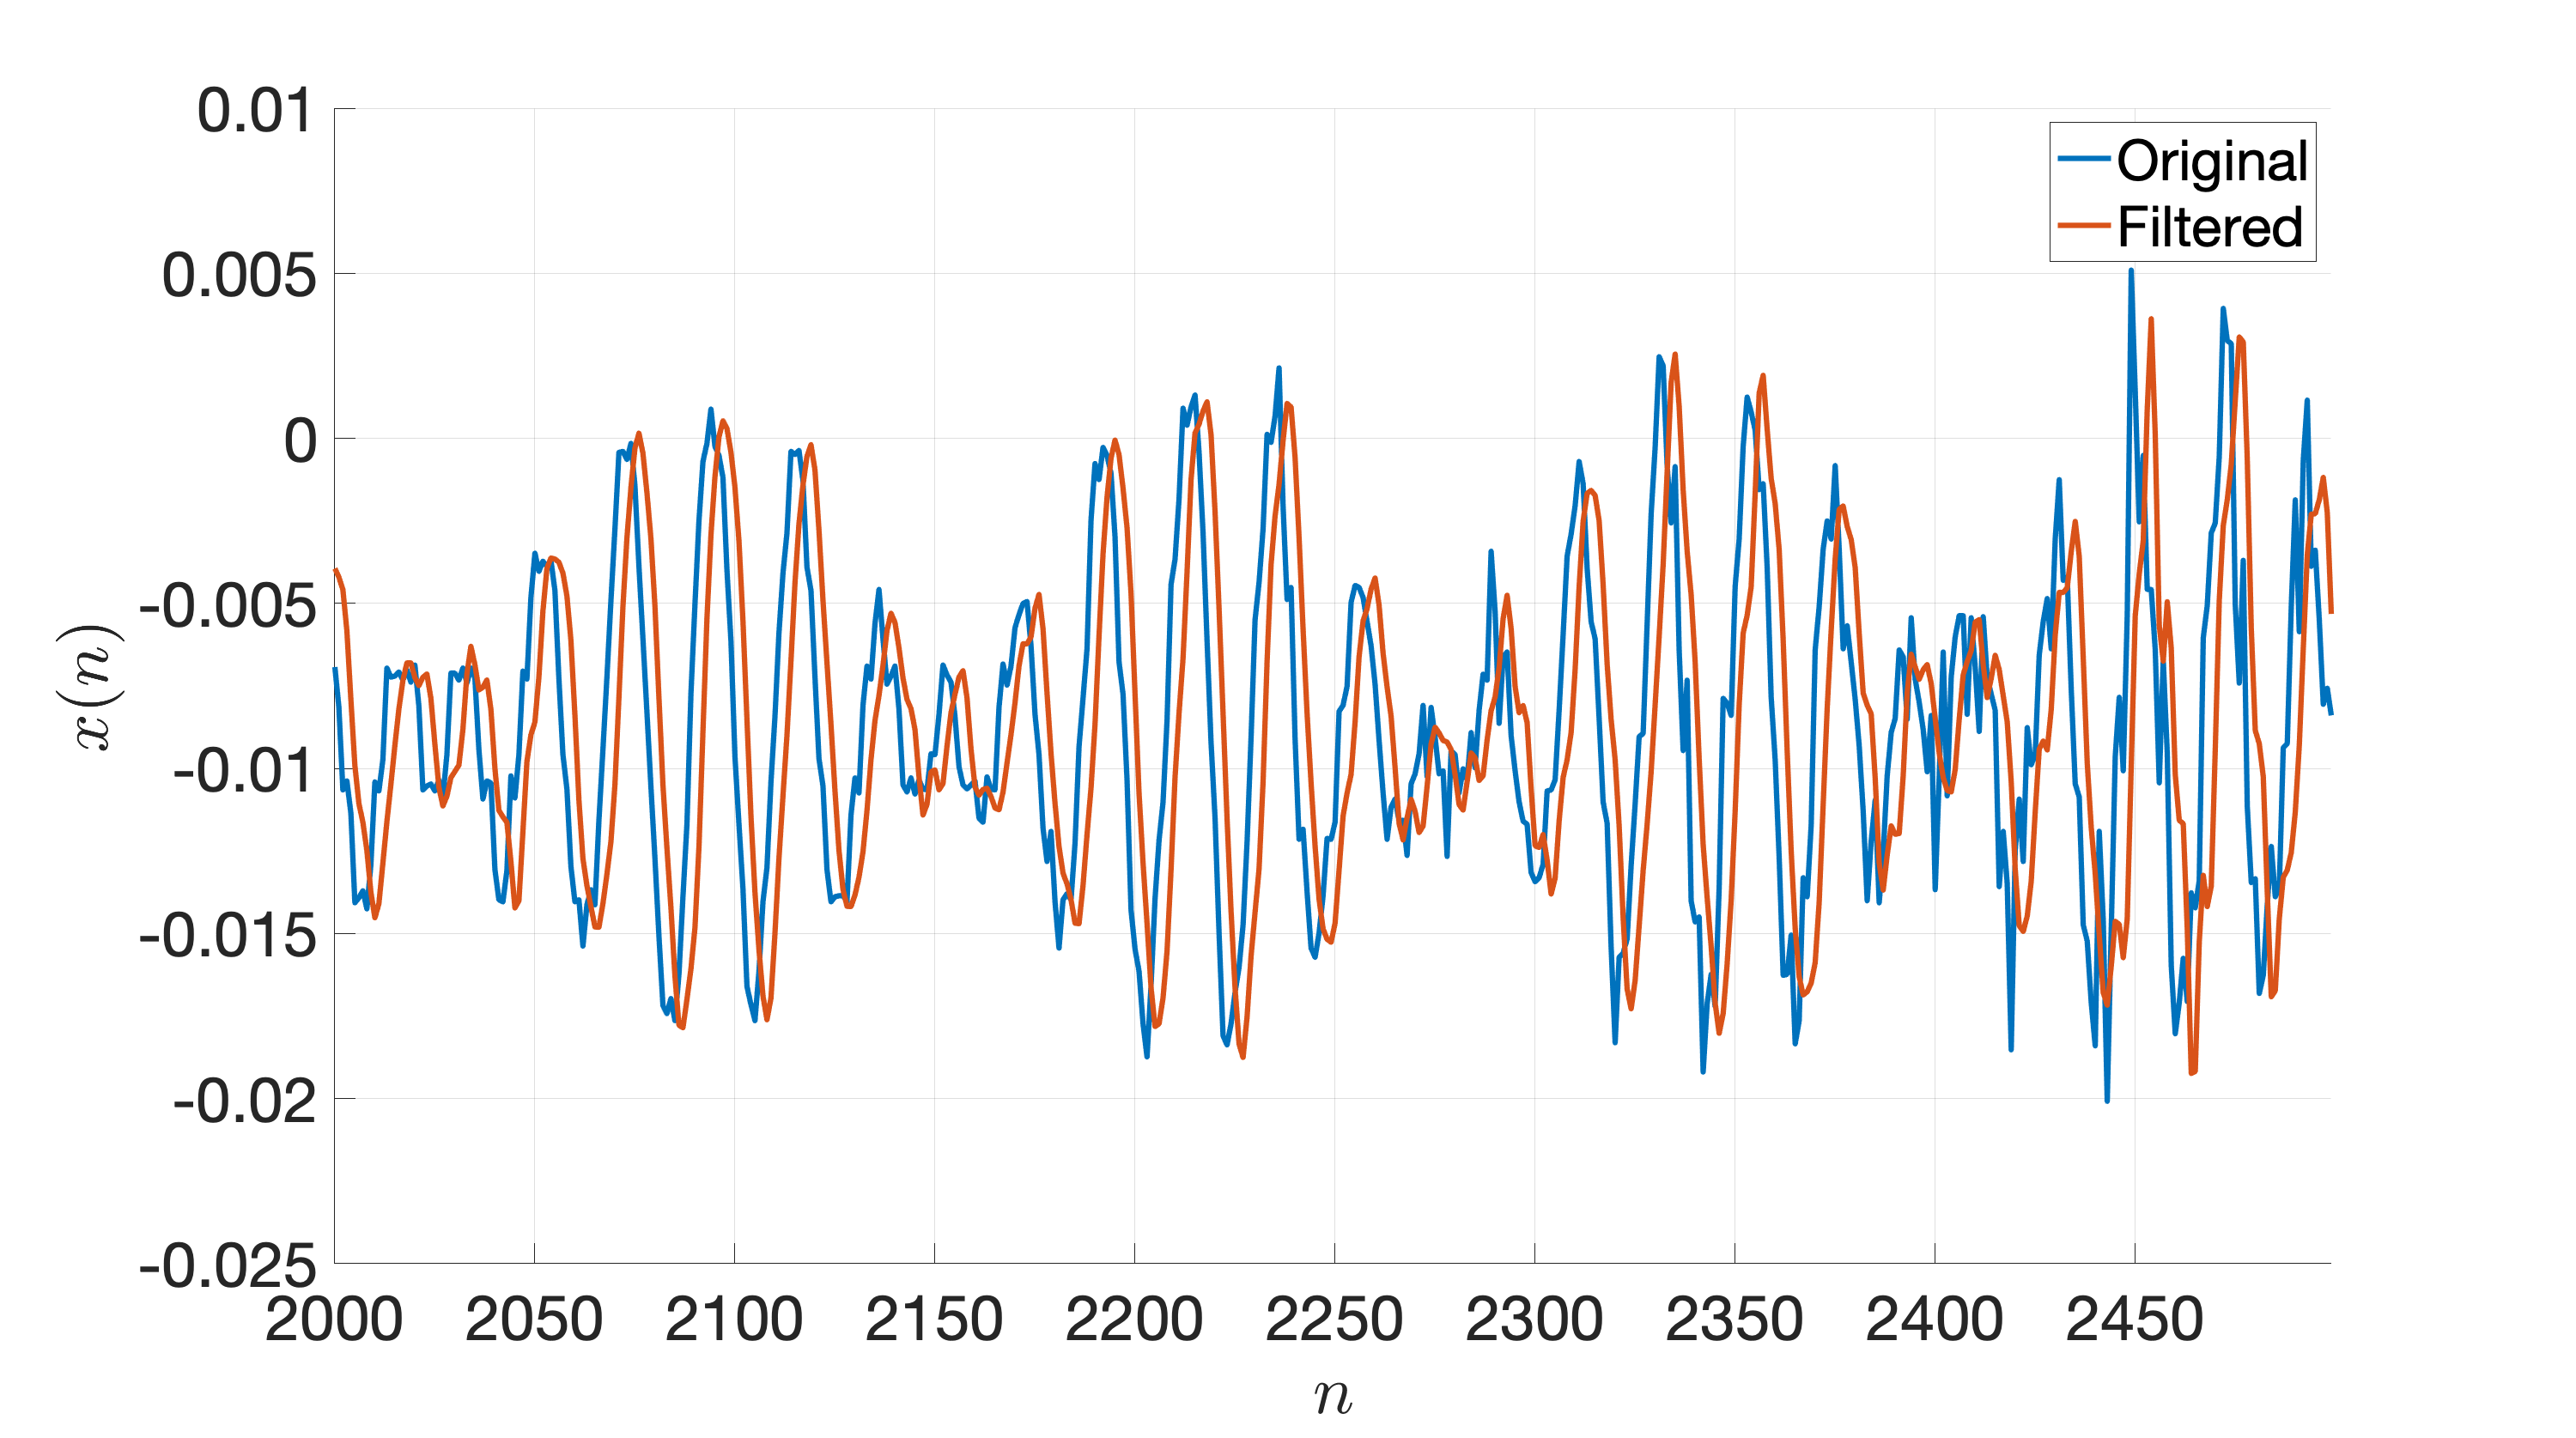
\includegraphics[width= 1.1\textwidth]{figures/R2c_zoomNormal.png}
	\caption{LTI filtered signal with $\omega_{co} = \pi/2$.}
	\label{fig:R2c_zoomNormal}
\end{minipage}
\end{figure}

\subsection{R2.d) Analysis of the filtered signal in the frequency domain}
Fig. \ref{fig:R2d} shows the comparison of the magnitude spectra of the original and filtered signals. As expected from the analysis of the gain of the filter (represented in Fig. \ref{fig:R2a_gain}), the components of the signal with frequency greater than the cutoff frequency (represented in Fig. \ref{fig:R2d} by a vertical dashed line) are attenuated. Nevertheless, given that the magnitude spectrum of the impulsive noise is spread evenly across all frequencies, it is evident that, with this filter, only a portion of the noise is attenuated. It is also important to remark, that noiseless components of higher frequencies are also attenuated contributing to the distortion and loss of sharpness in the sound of the filtered signal. Furthermore, Fig. \ref{fig:Red_spectrogram} shows the spectrogram of the filtered signal for the segment of Fig. \ref{fig:R1b}. As put forward previously, the constant power vertical noise of the lines remain unchanged for lower frequencies, thus this filter was not able to filter the signal adequately.

\begin{figure}[htbp]
	\centering
	\begin{minipage}[b]{.49\textwidth}
		\centering
		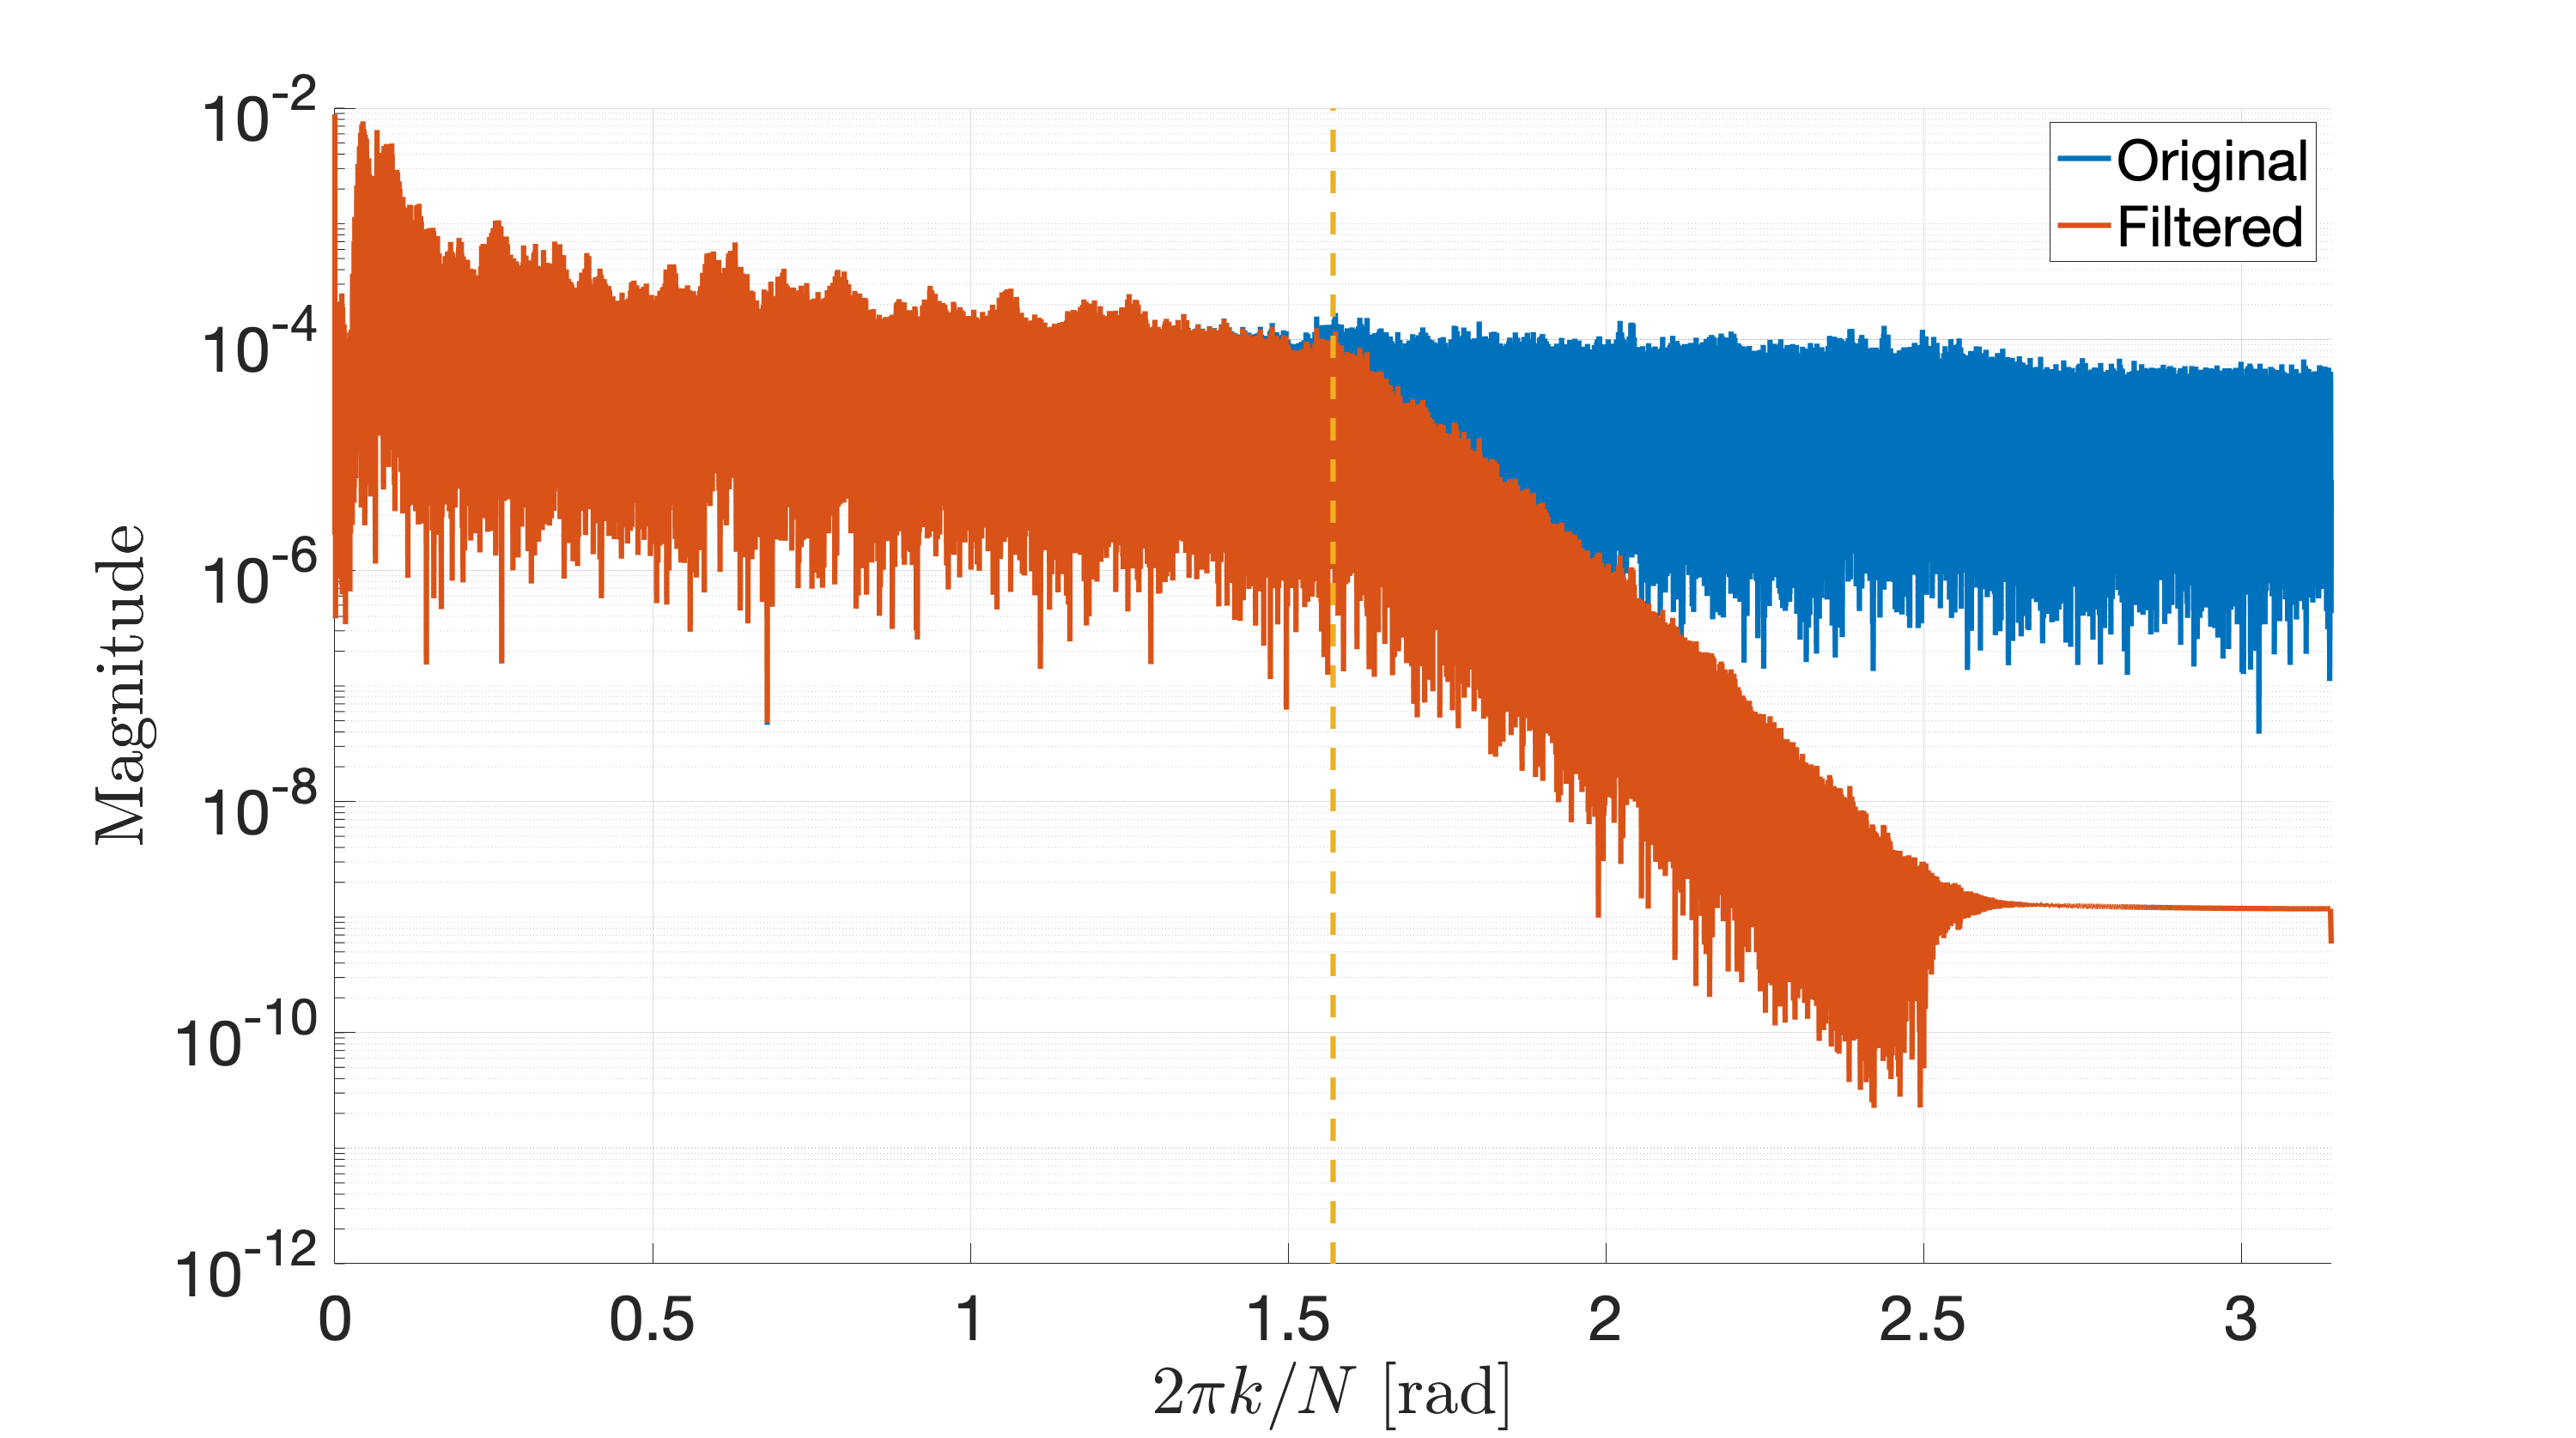
\includegraphics[width= 1.1\textwidth]{figures/R2d.png}
		\caption{Magnitude spectrum of the original and filtered sound signals.}
		\label{fig:R2d}
	\end{minipage}
	\hfill
	\begin{minipage}[b]{.49\textwidth}
		\centering
		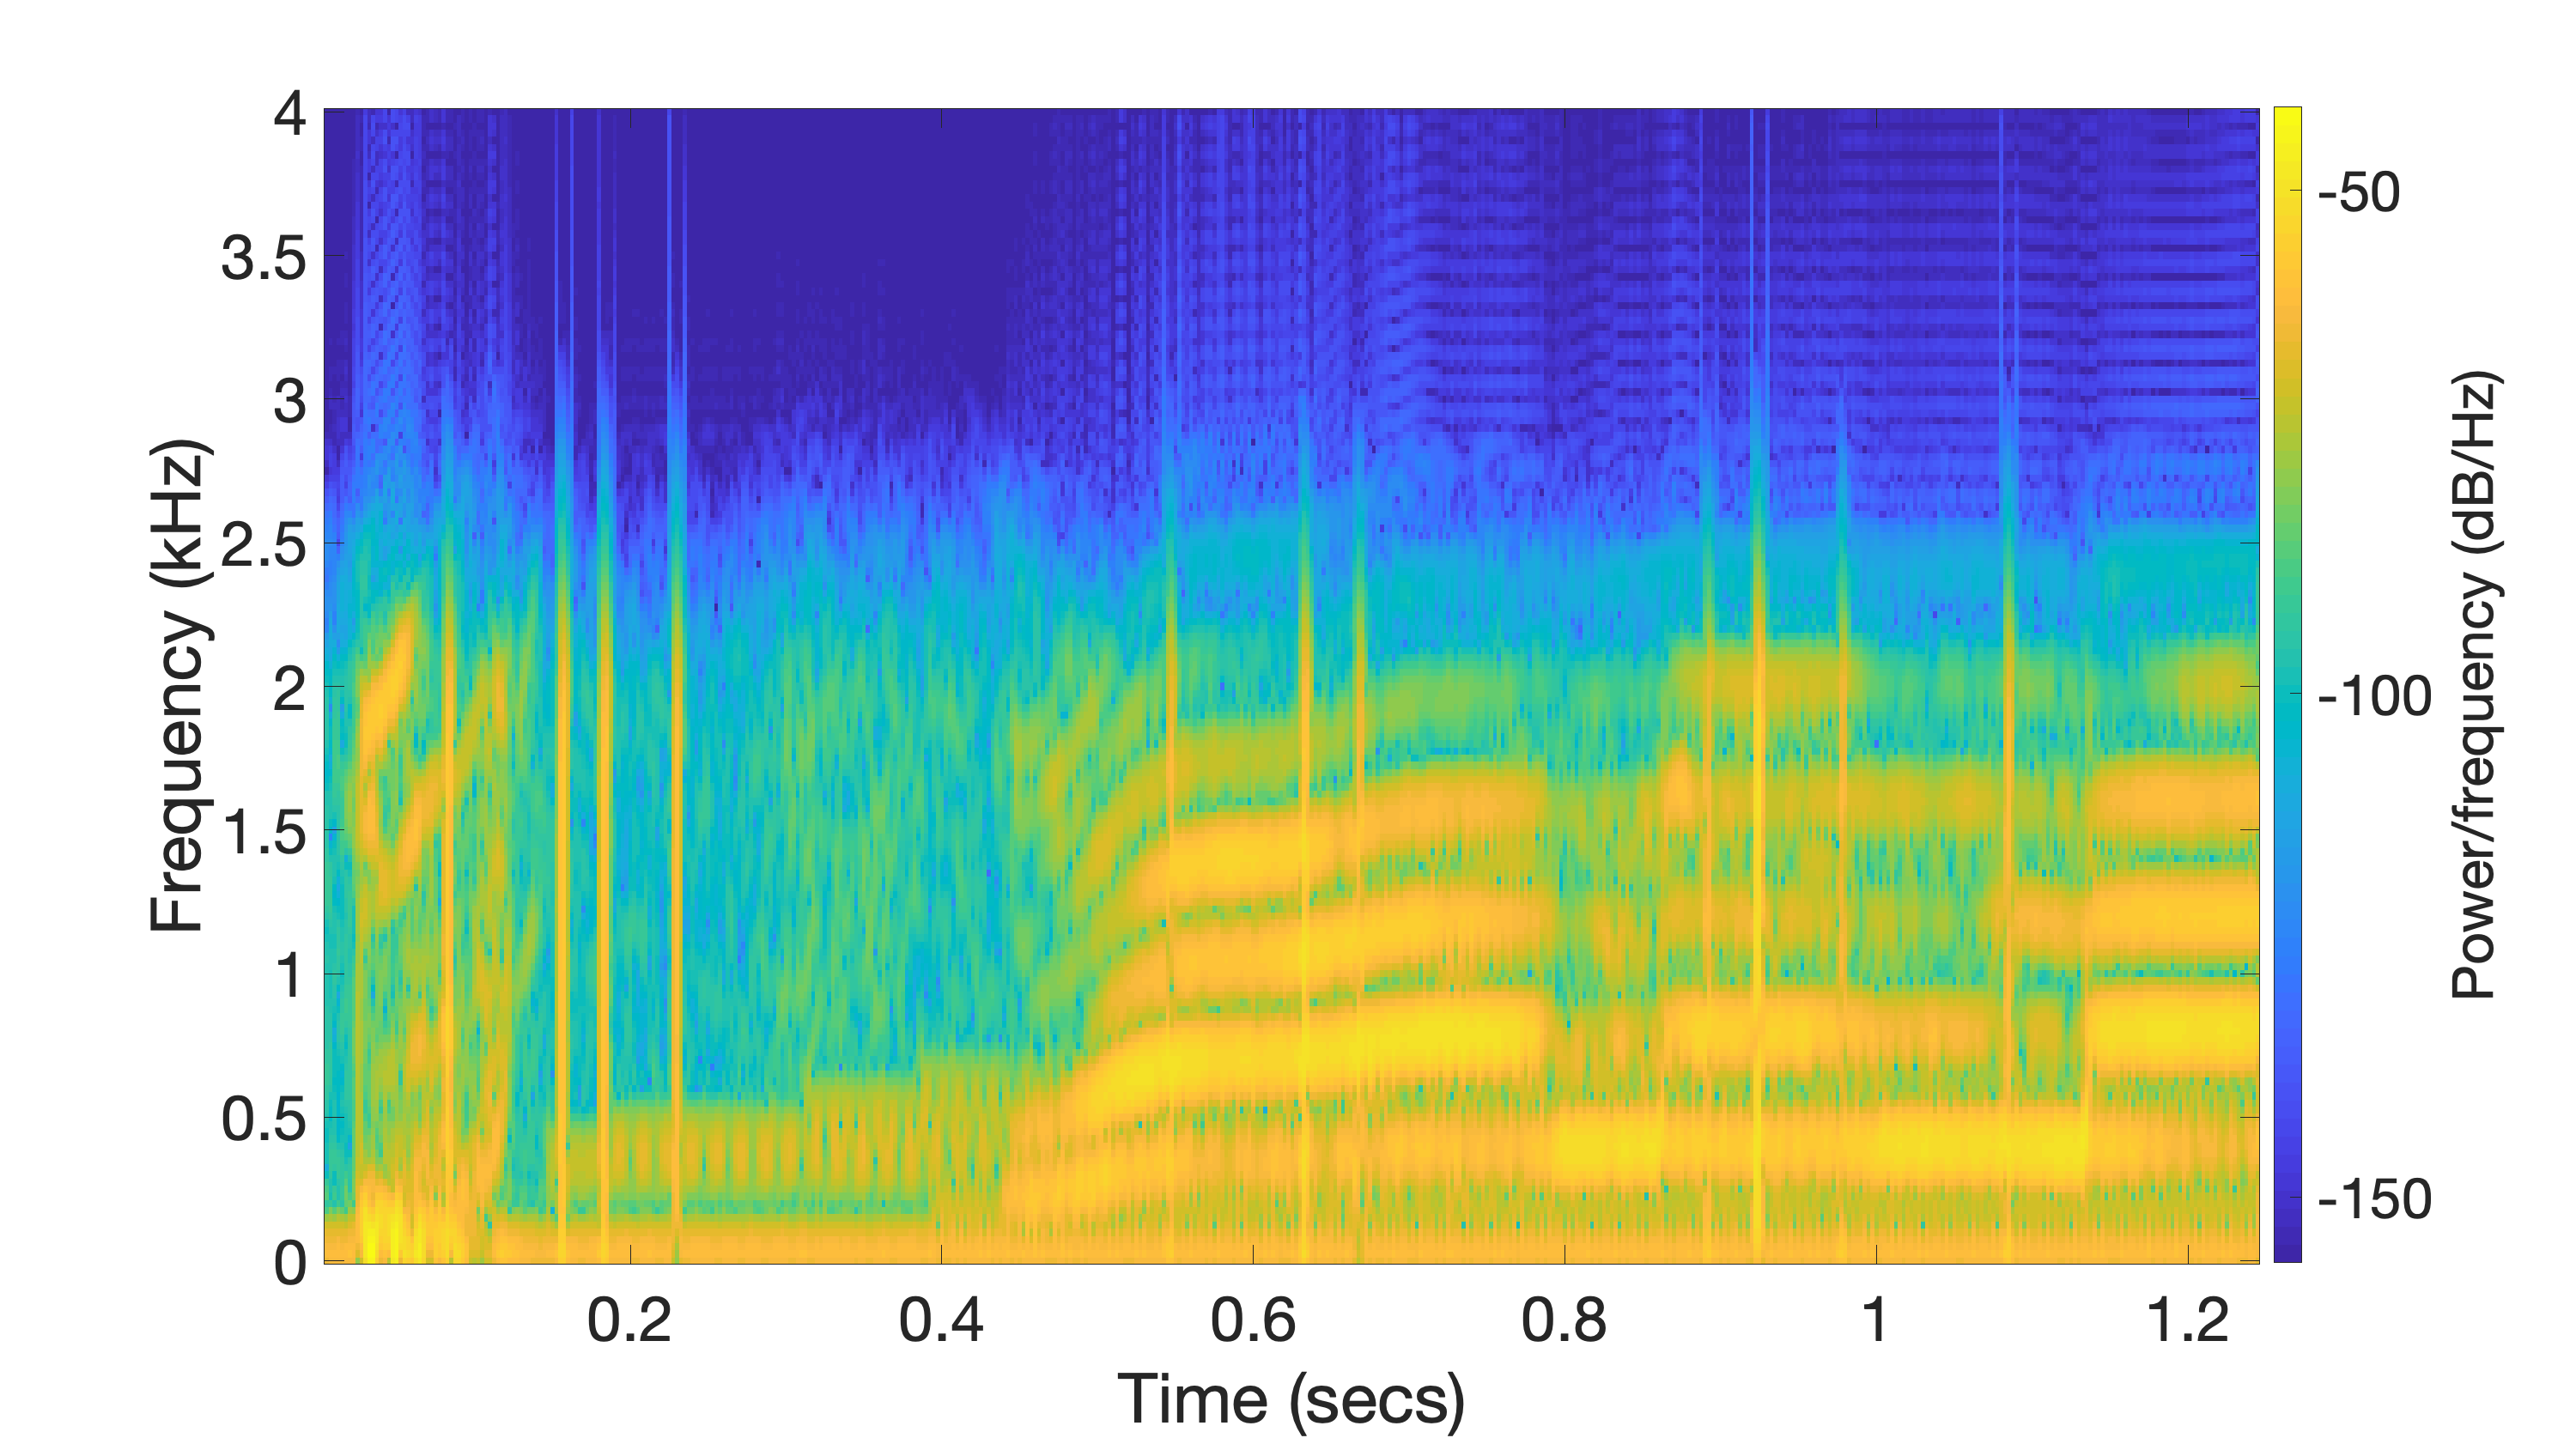
\includegraphics[width= 1.1\textwidth]{figures/R2d_spectrogram.png}
		\caption{Spectrogram of the filtered signal the segment of Fig. \ref{fig:R1b}.}
		\label{fig:Red_spectrogram}
	\end{minipage}
\end{figure}

\subsection{R2.e) Listening to the filtered signal}
Listening to the filtered signal it is possible to conclude that the attenuation on the impulsive noise is very unsatisfactory, given that the noise impulses are still very clear and loud. Furthermore, there is a loss of sharpness in the song because of the phenomena put forward in the two previous subsections.

\subsection{R2.f) Improving Butterworth low-pass filter}

The Butterworth filter operates on frequency, but as seen in Section \ref{sec:R1}, it is very difficult to identify and isolate the noise in the frequency domain. It is, thus, expected that the performance of such a filter is poor, as noticed so far. Given that in the magnitude spectrum the noise impulses are spread evenly across all frequencies, the only way of attenuating the impulsive noise is to decrease the cutoff frequency of the filter. This solution results, however, in the degradation of the quality of the song. Using this filter for this particular noise reduces to a trade-off between degradation of quality and noise attenuation. Synthesizing a filter with cutoff frequency $\omega_{co} = \pi/4$, the filtered signal is characterized in Figs. \ref{fig:Rfc}--\ref{fig:R2f_spectrogram}. 

First, it is seen in Fig. \ref{fig:Rfc} that the noise impulses are more attenuated in relation to Fig. \ref{fig:R2c}. However, they are still very significant. This is expected, since a larger portion of component of the constant magnitude spectrum of the noise signal was attenuated. However, some segments of the signal which are not corrupted by noise are attenuated and, thus, distorted. Second, in Fig. \ref{fig:R2f_zoomNoise} it is possible to analyze the behavior of the filter after a noise impulse in the time domain. After the noise impulse, as expected, the response of the noiseless signal is still superimposed with the impulse response of the filter, which is still similar to the response of an under-damped second order system with a lower natural frequency. Third, in Fig. \ref{fig:R2c_zoomNormal} it is possible to notice that the delay introduced by the filter increased. Fourth, from Figs. \ref{fig:R2f} and \ref{fig:R2f_spectrogram}, given that the magnitude spectrum of the impulsive noise is spread evenly across all frequencies, it is evident that with this filter still only a portion, albeit larger, of the noise is attenuated. It is also important to remark, that noiseless components of the signal are even more attenuated, contributing to a greater distortion and loss of sharpness in the sound of the filtered signal.
\begin{figure}[htbp]
	\centering
	\begin{minipage}[b]{.49\textwidth}
		\centering
		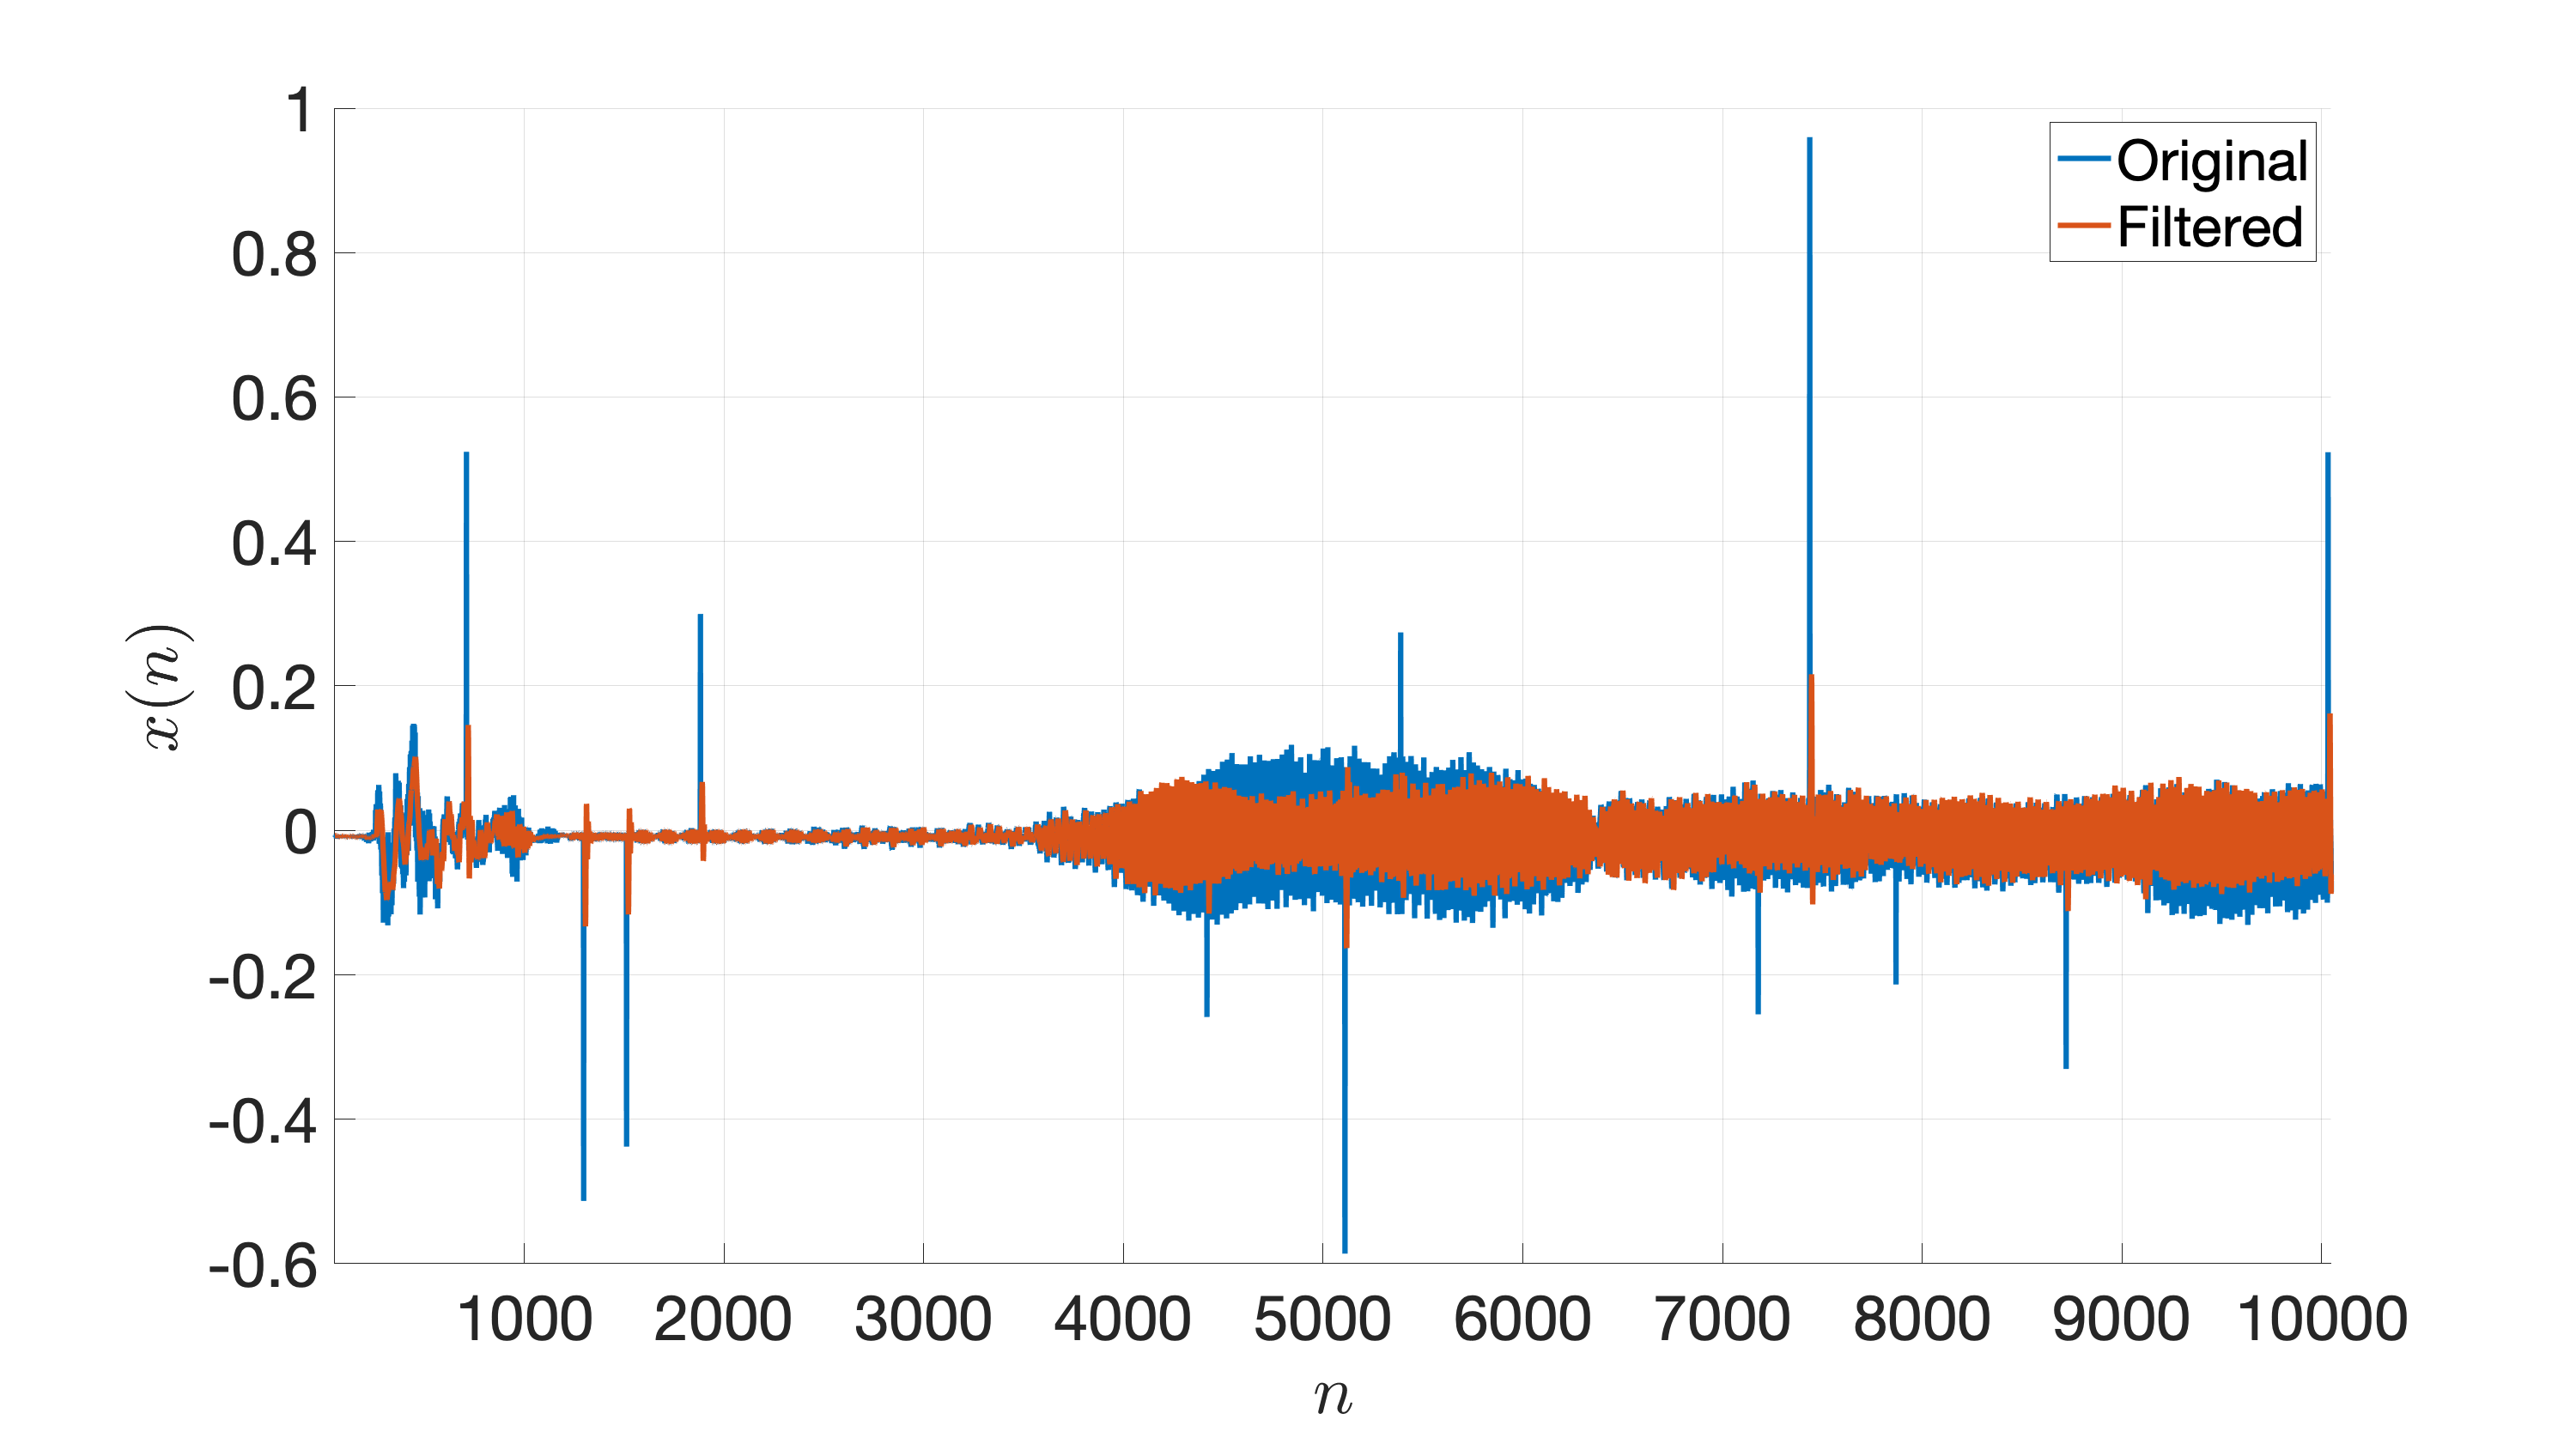
\includegraphics[width= 1.1\textwidth]{figures/R2f_zoomOut.png}
		\caption{LTI filtered signal with $\omega_{co} = \pi/4$.}
		\label{fig:Rfc}
	\end{minipage}
	\hfill
	\begin{minipage}[b]{.49\textwidth}
		\centering
		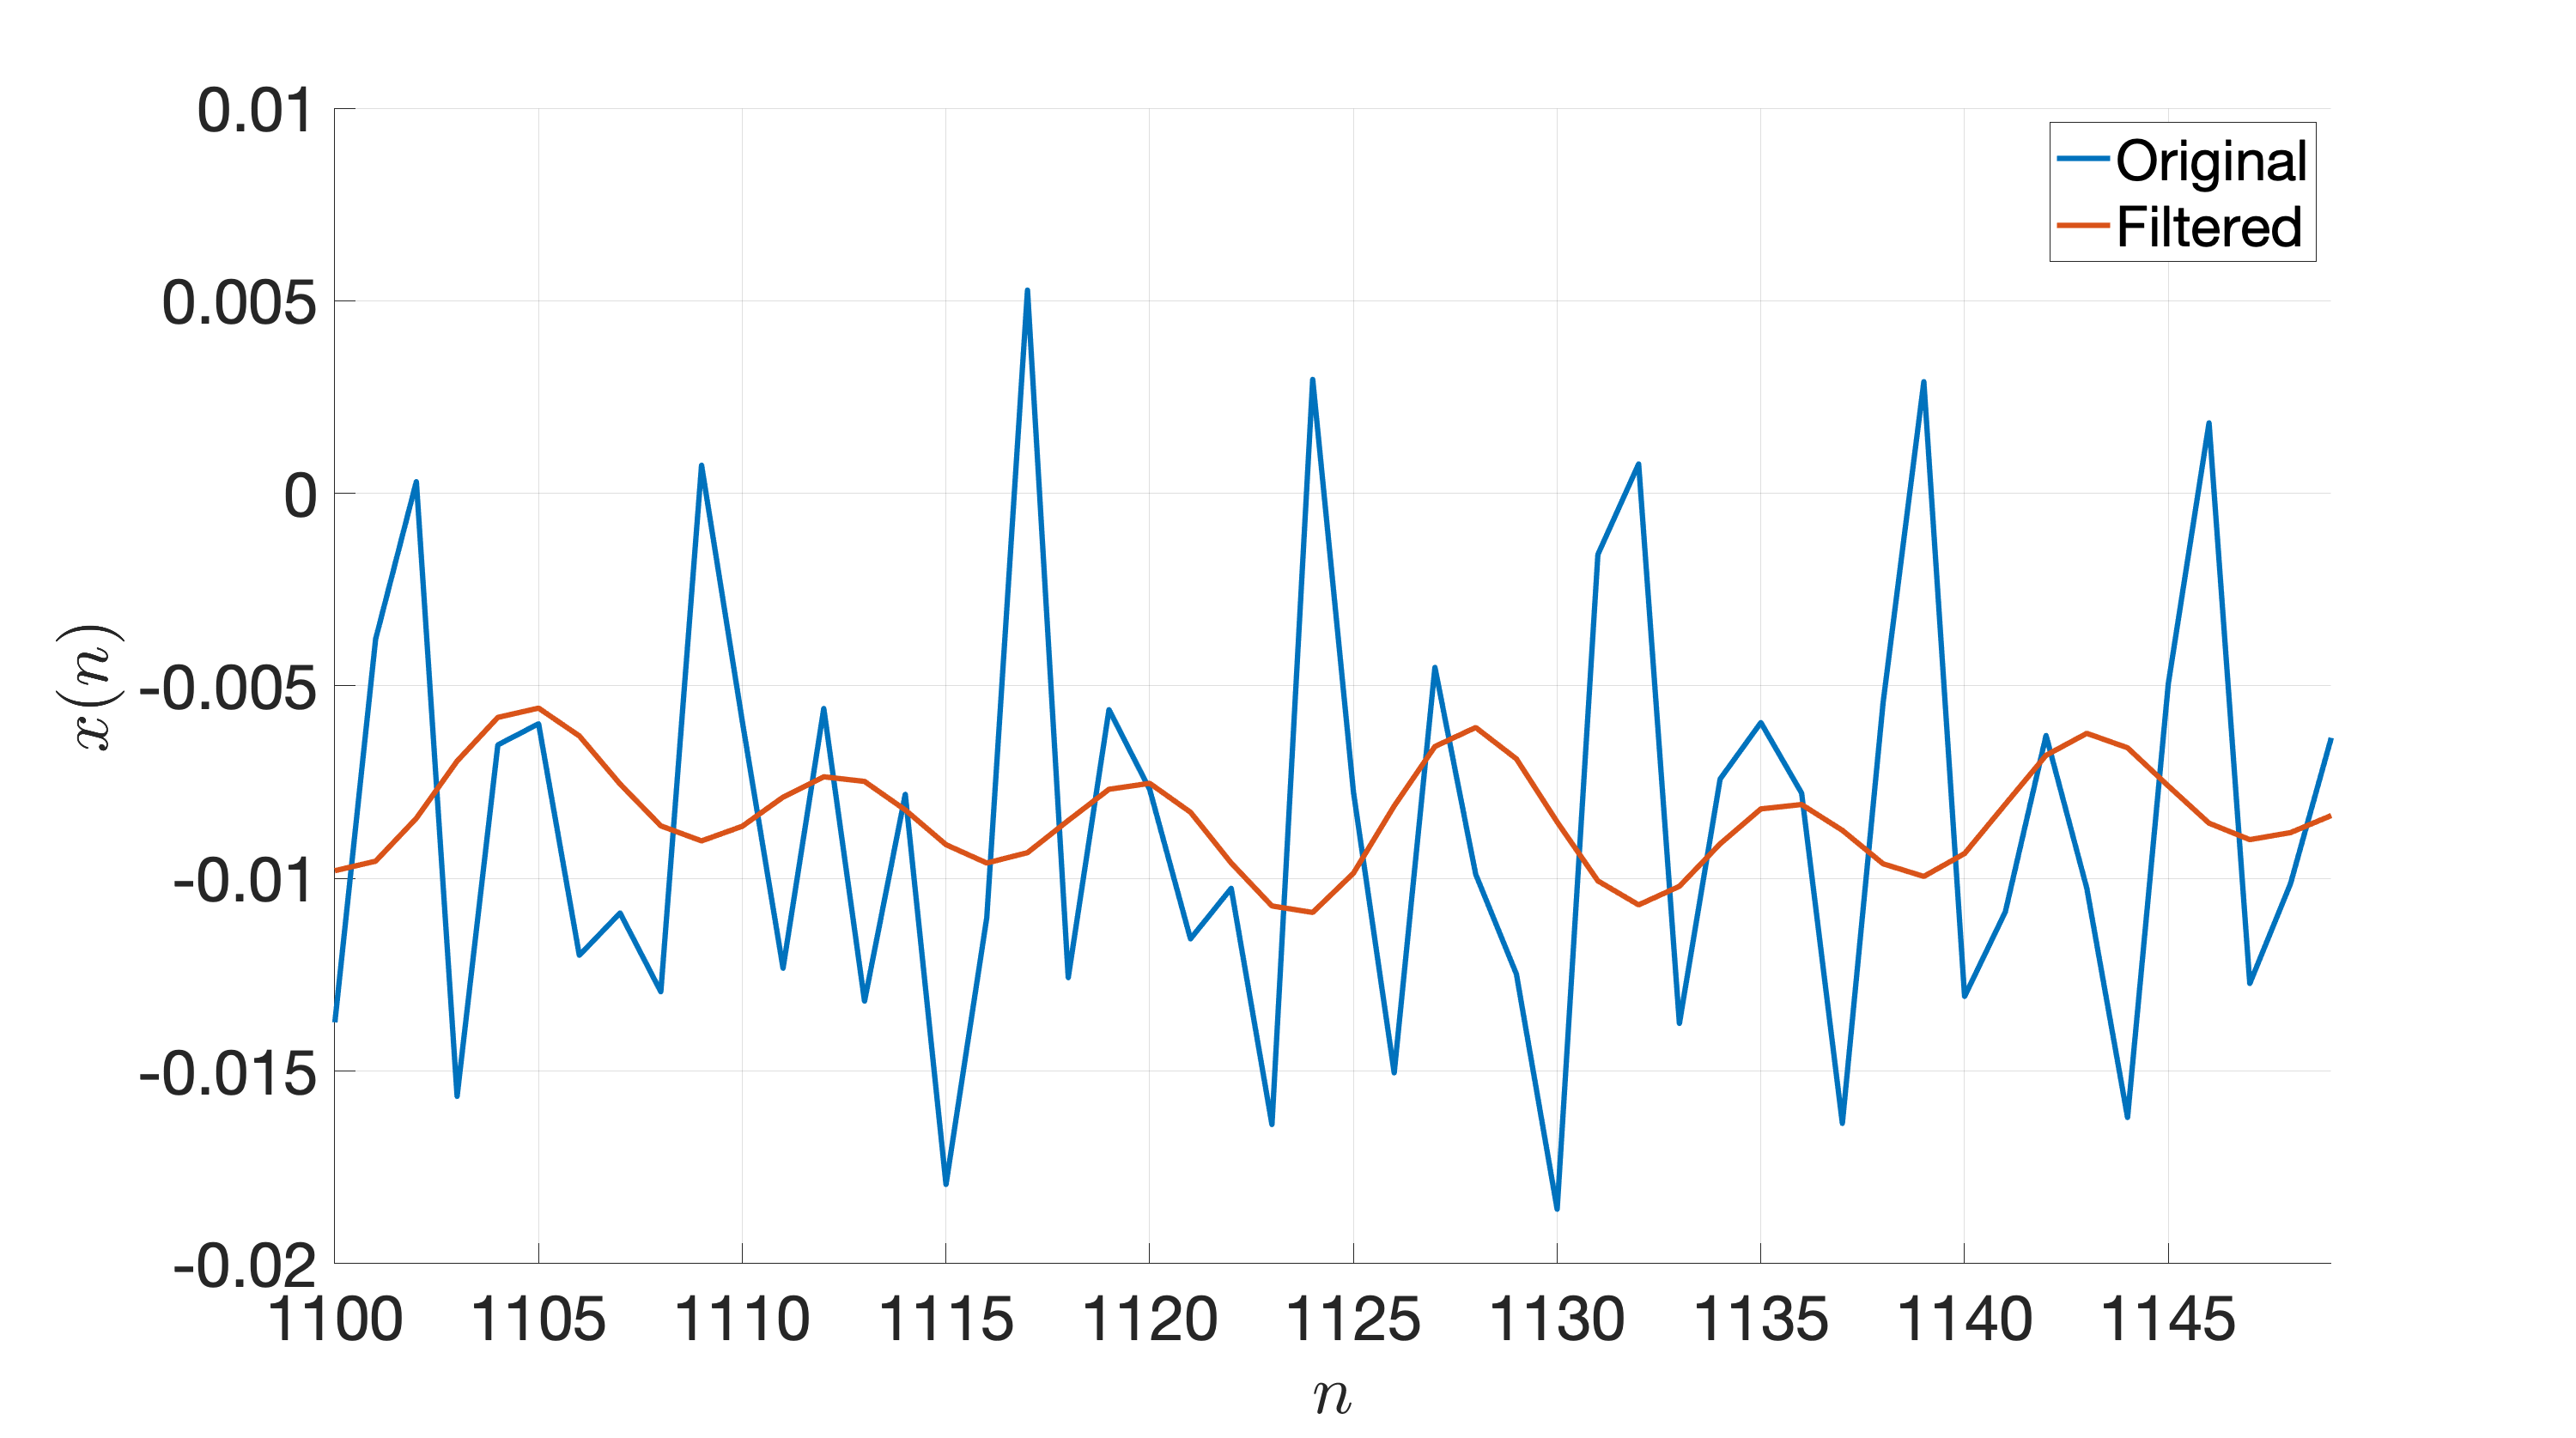
\includegraphics[width= 1.1\textwidth]{figures/R2f_smallAmp.png}
		\caption{LTI filtered signal with $\omega_{co} = \pi/4$.}
		\label{fig:R2f_smallAmp}
	\end{minipage}
	\begin{minipage}[b]{.49\textwidth}
		\centering
		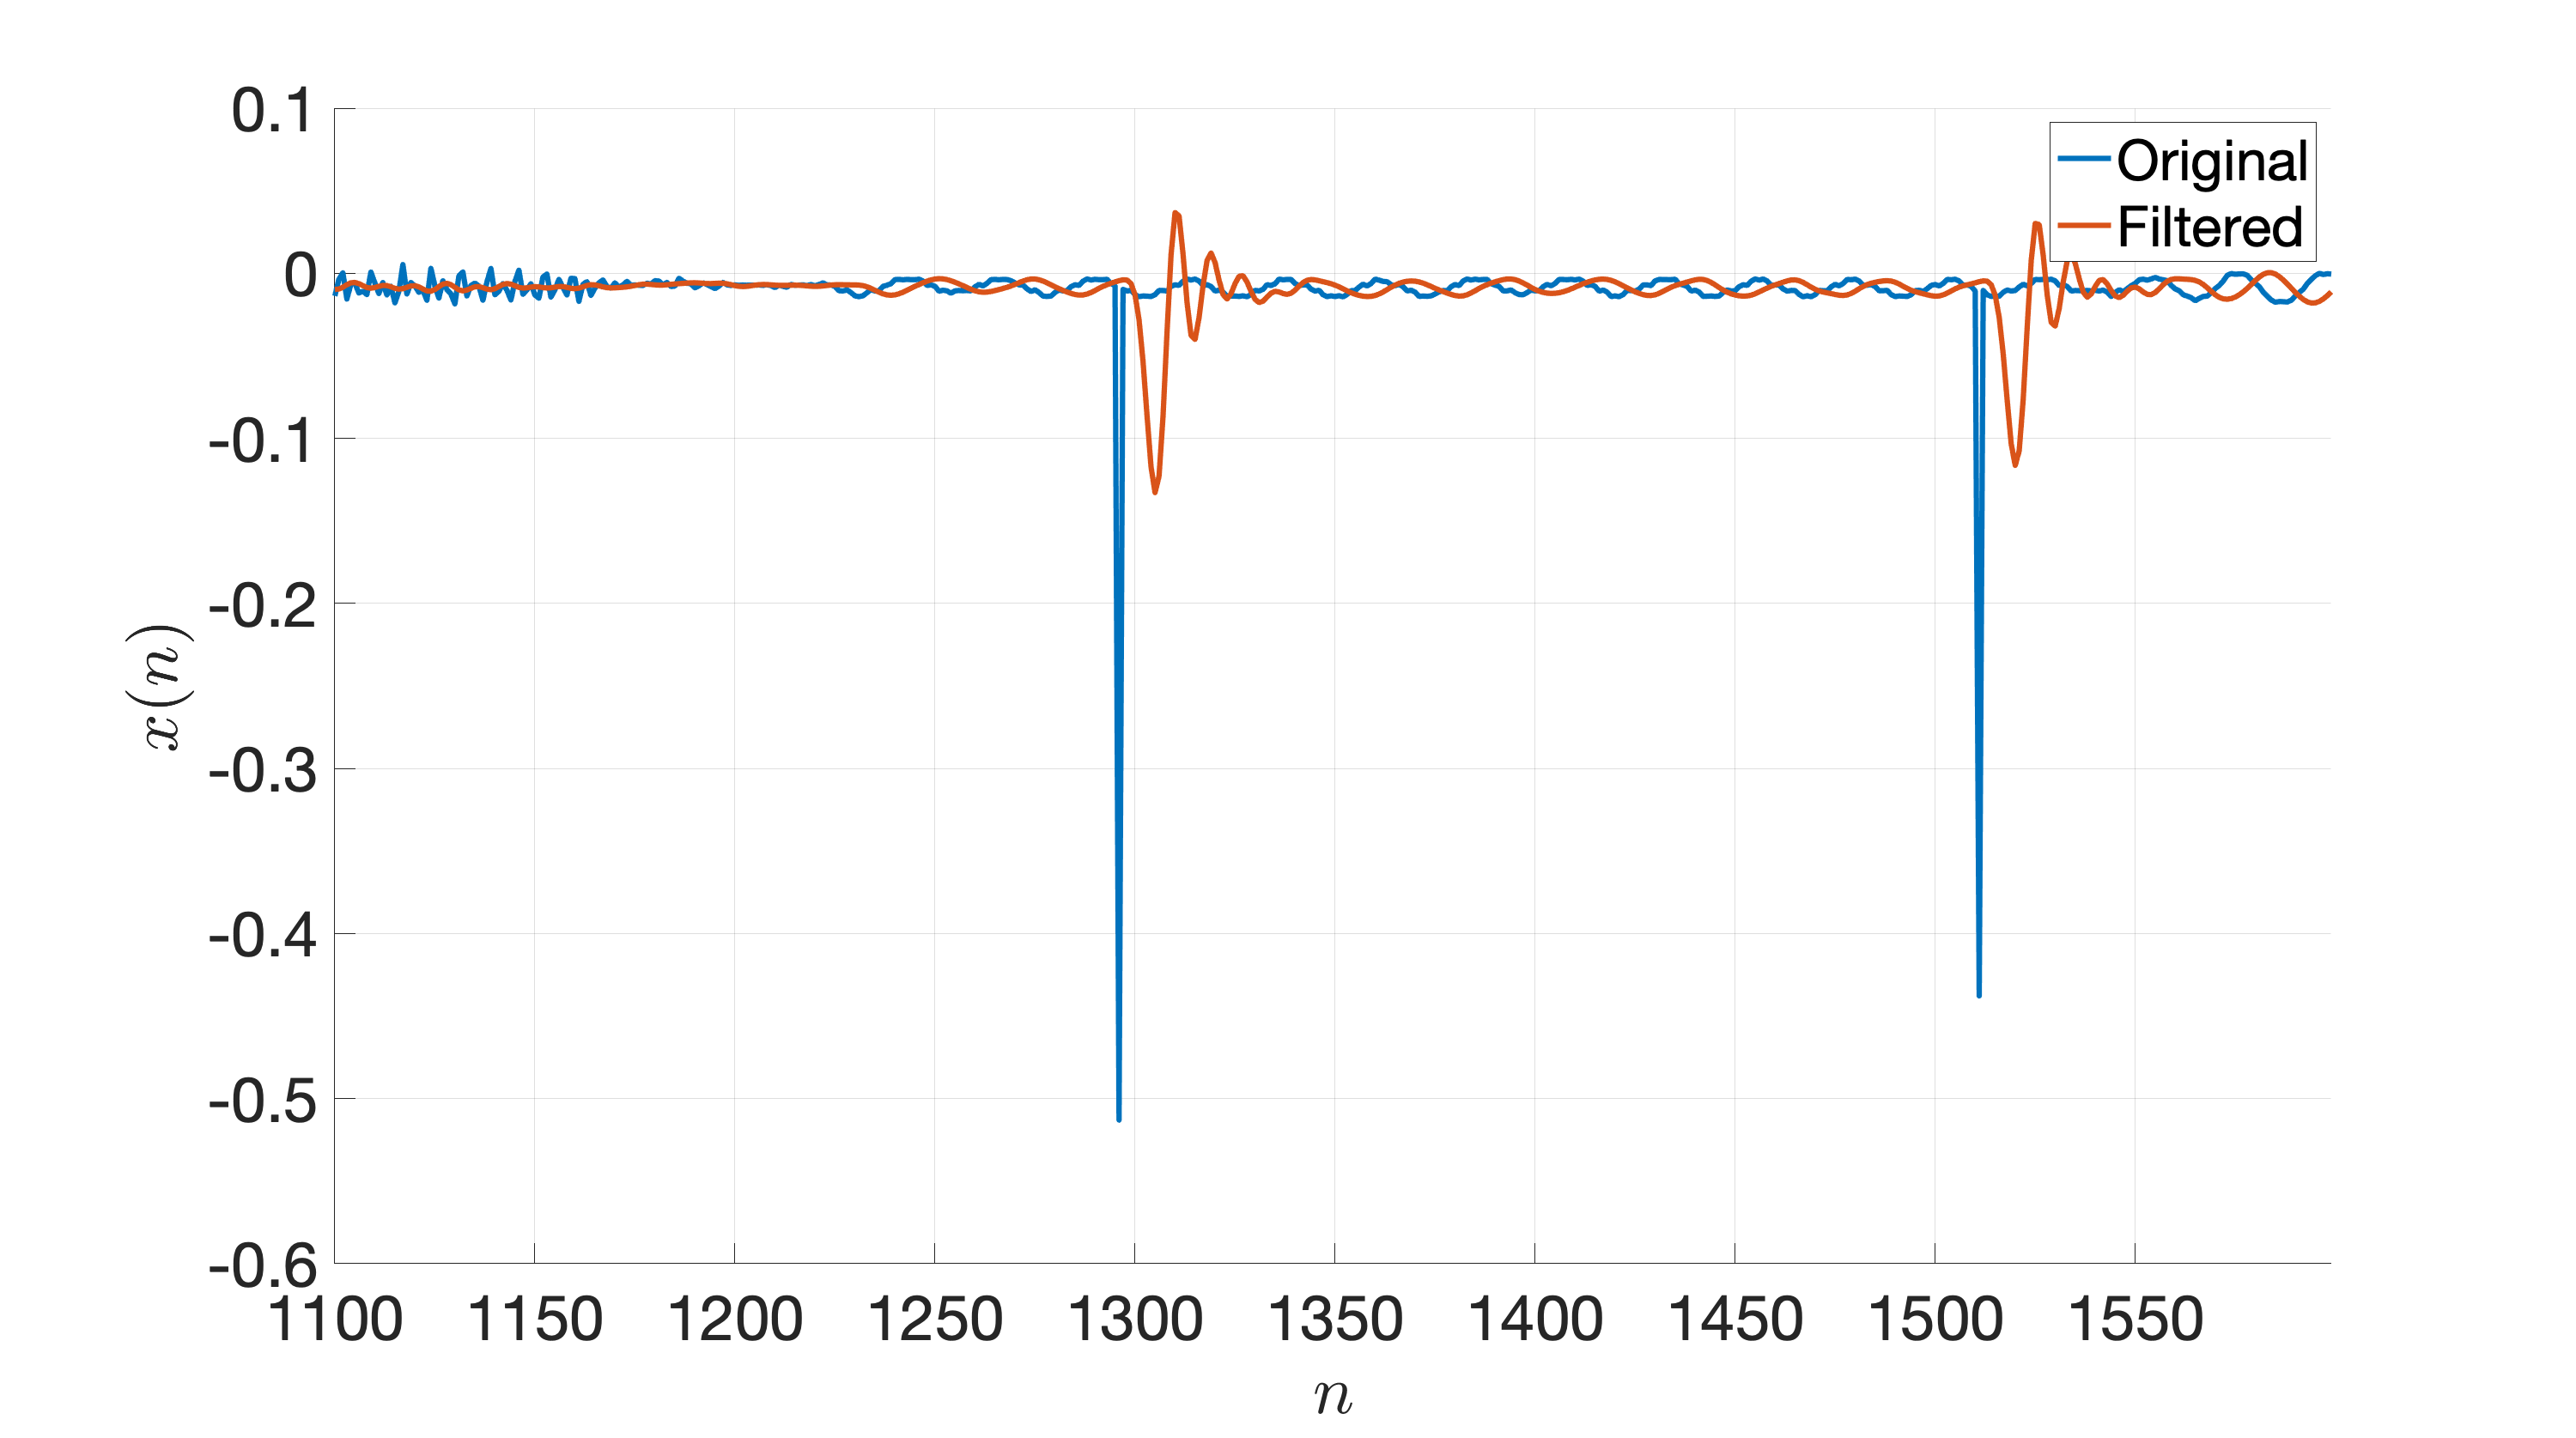
\includegraphics[width= 1.1\textwidth]{figures/R2f_zoomNoise.png}
		\caption{LTI filtered signal with $\omega_{co} = \pi/4$.}
		\label{fig:R2f_zoomNoise}
	\end{minipage}
	\hfill
	\begin{minipage}[b]{.49\textwidth}
		\centering
		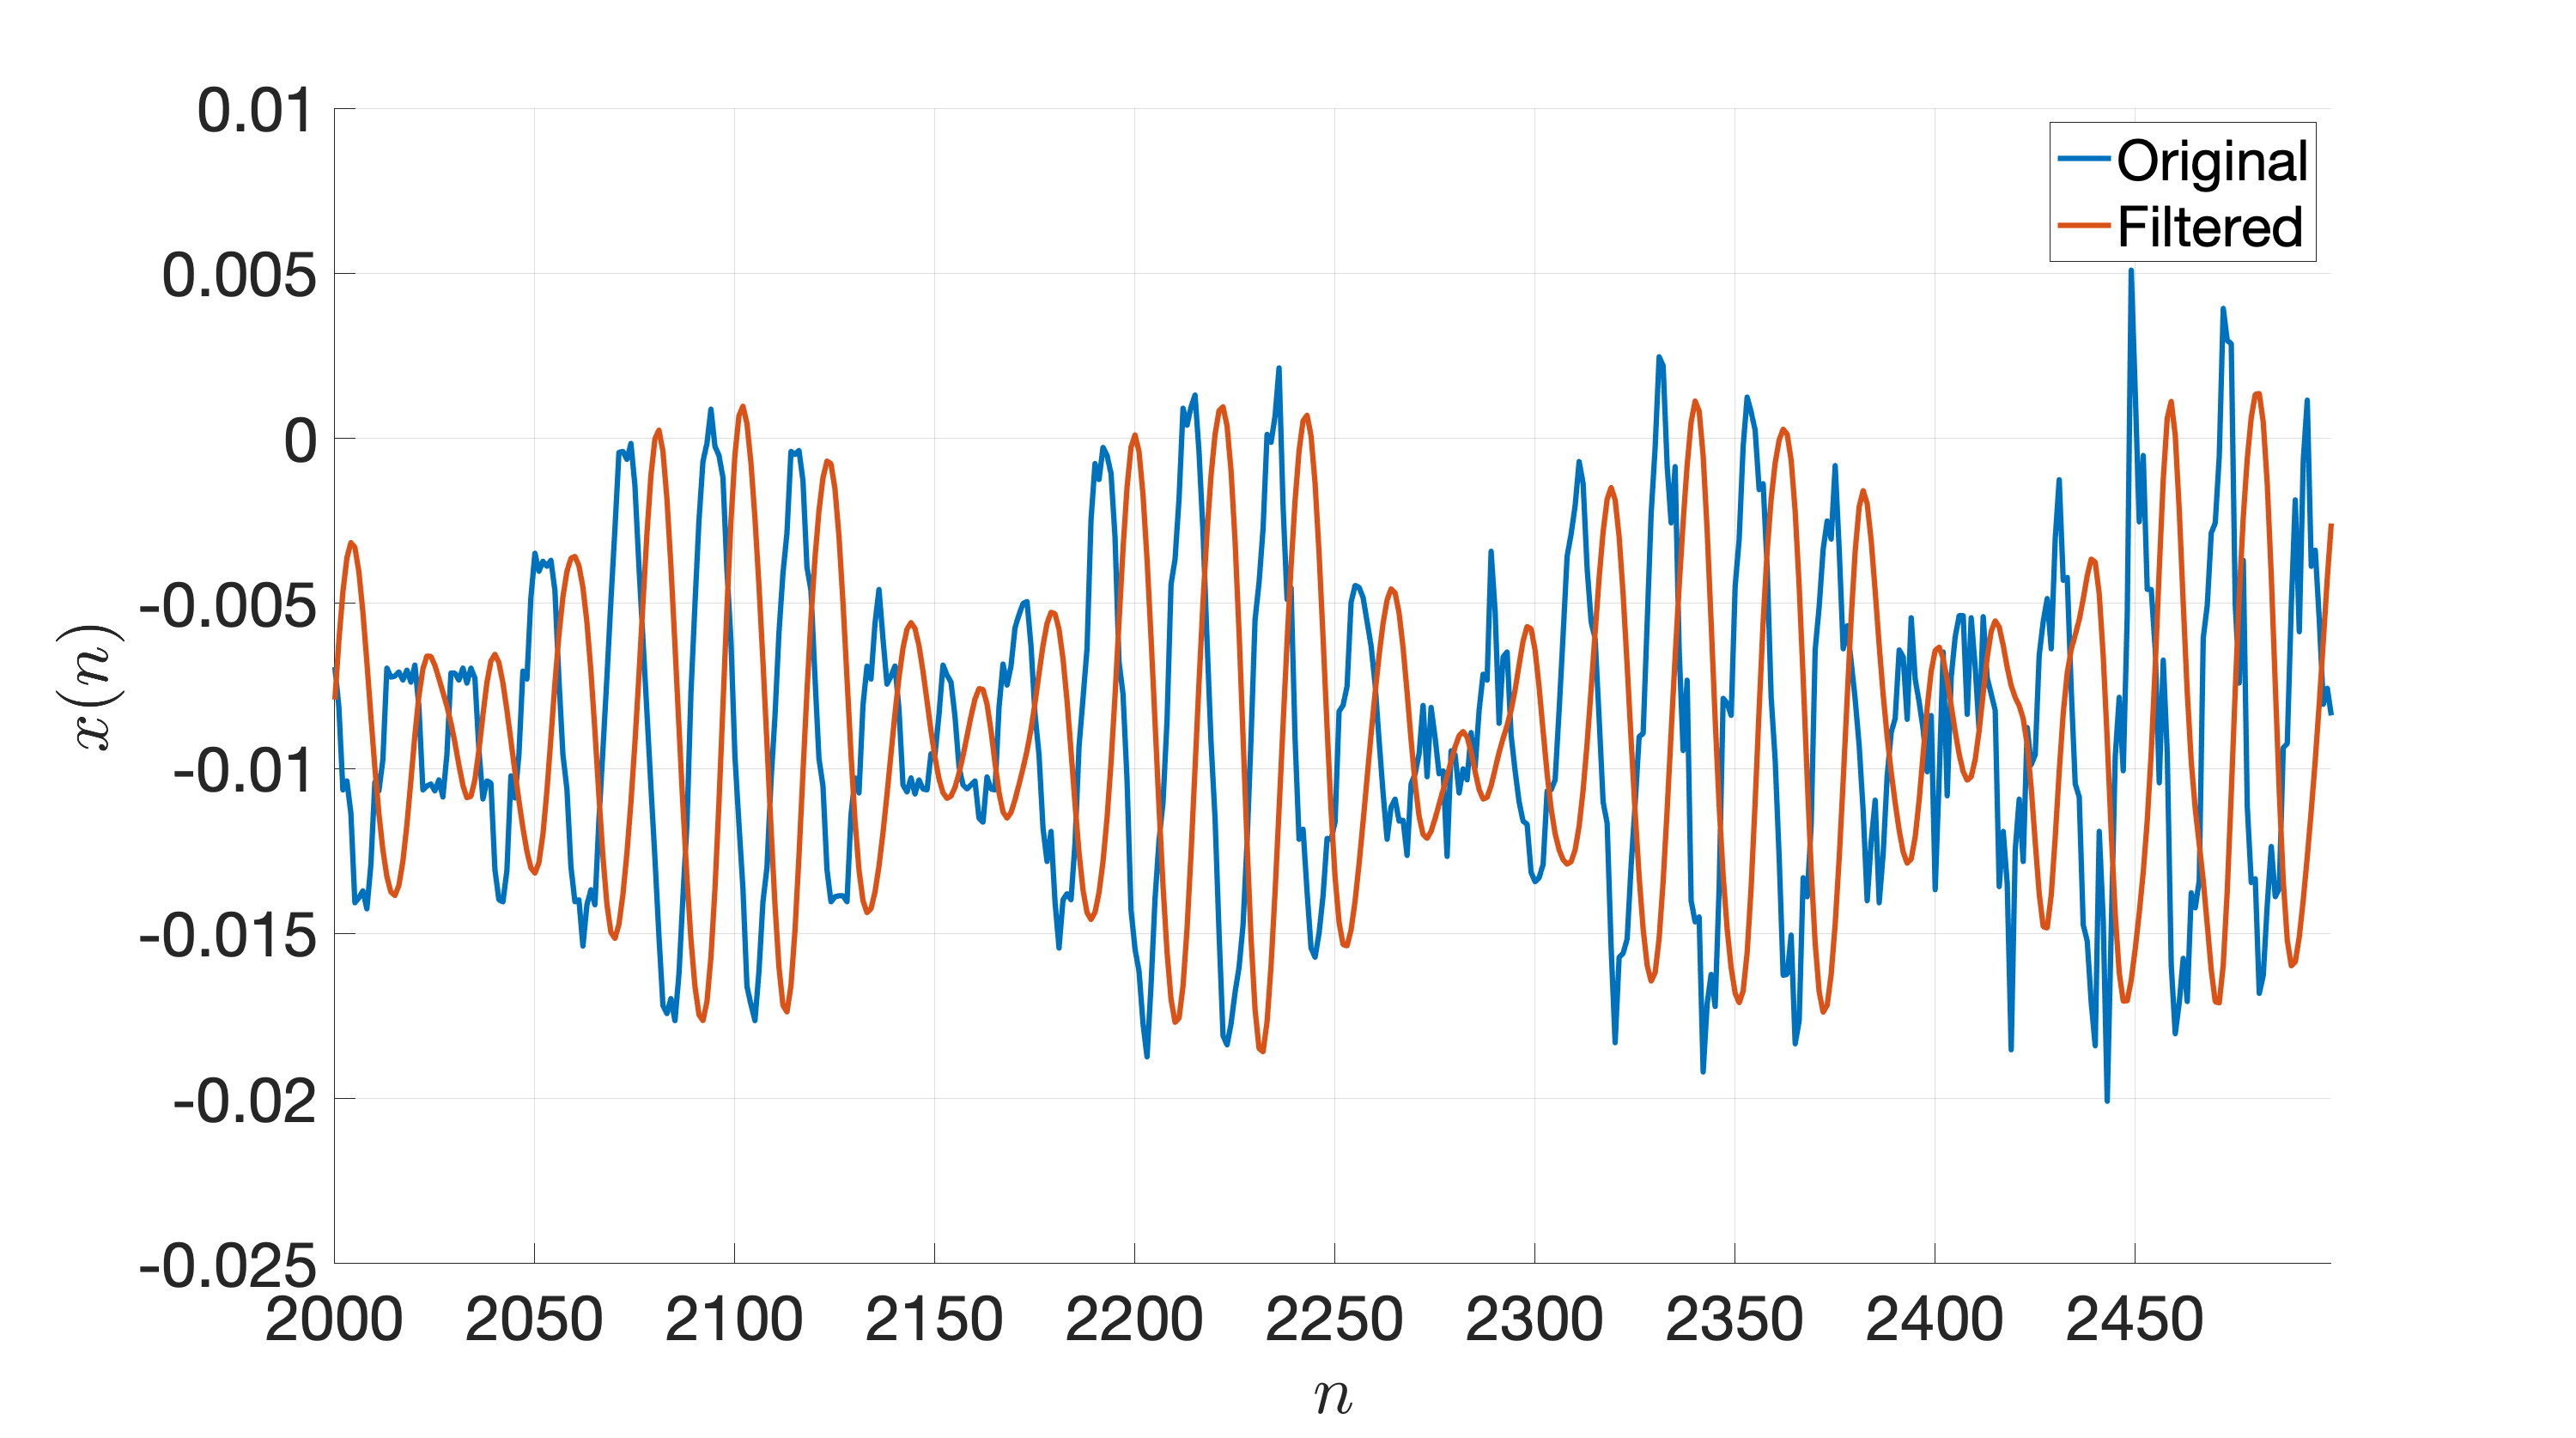
\includegraphics[width= 1.1\textwidth]{figures/R2f_zoomNormal.png}
		\caption{LTI filtered signal with $\omega_{co} = \pi/4$.}
		\label{fig:R2f_zoomNormal}
	\end{minipage}
\begin{minipage}[b]{.49\textwidth}
	\centering
	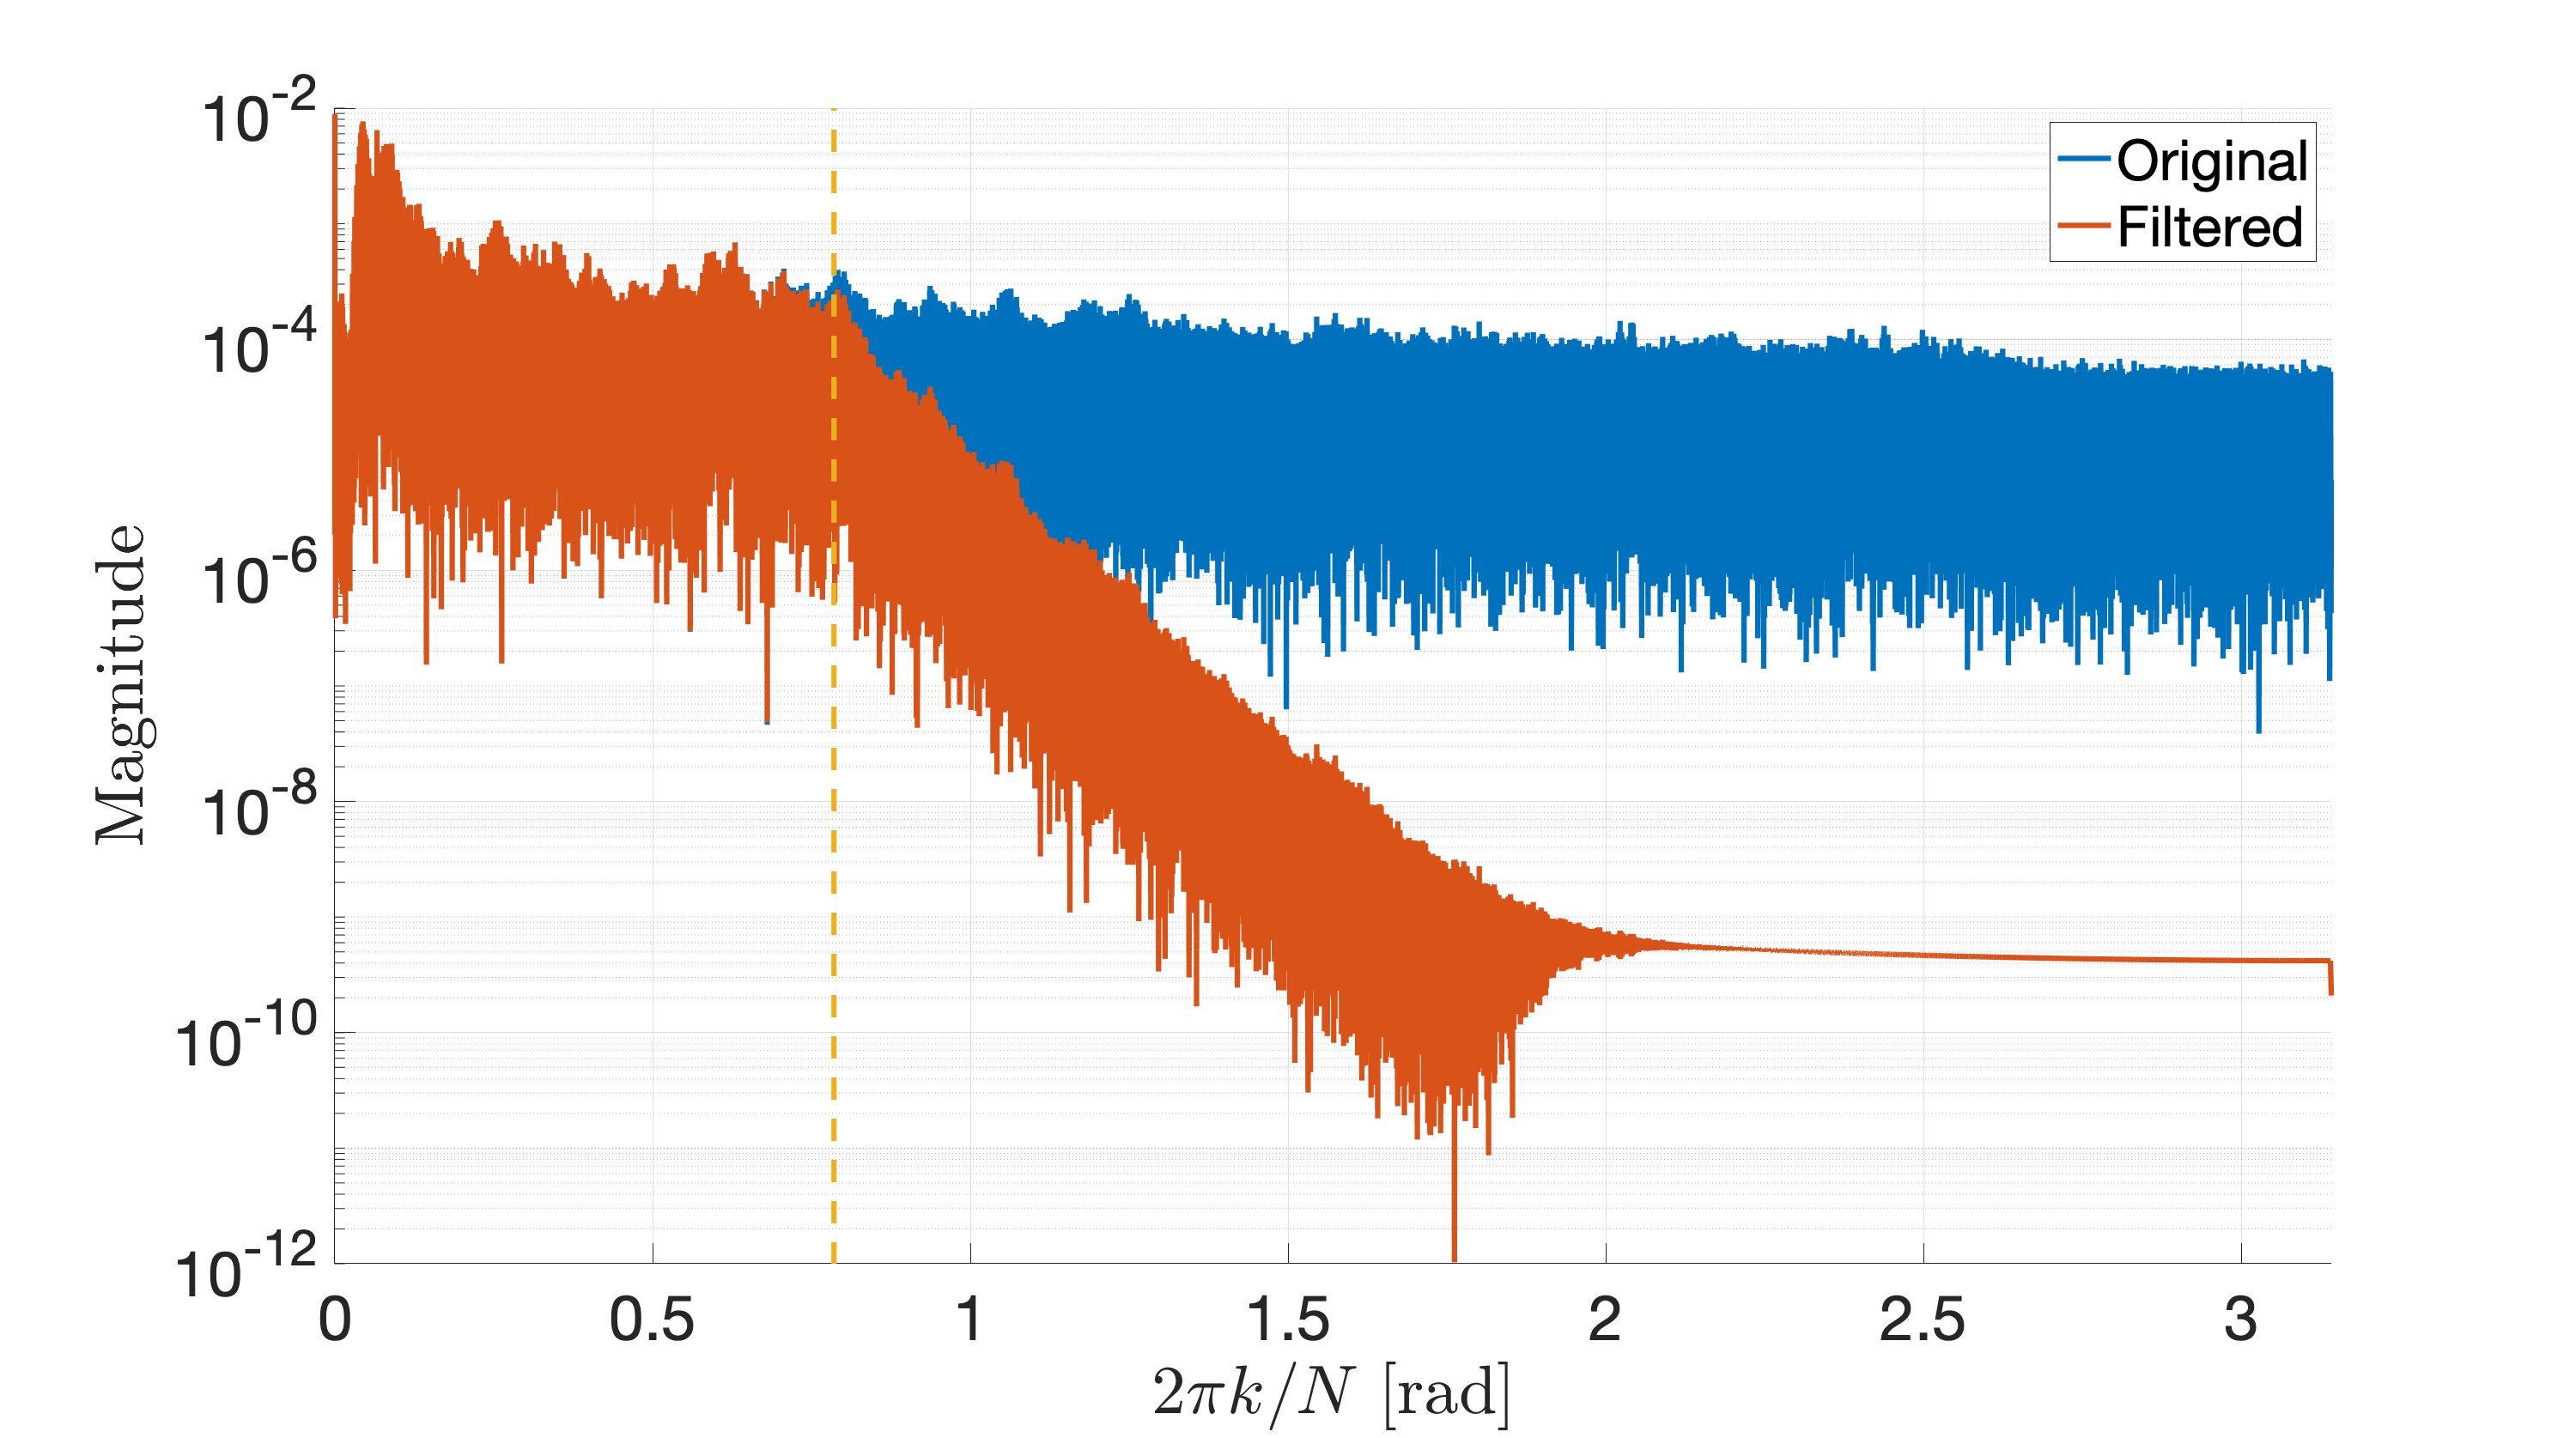
\includegraphics[width= 1.1\textwidth]{figures/R2f_spectra.png}
	\caption{Magnitude spectrum of the original and filtered sound signals.}
	\label{fig:R2f}
\end{minipage}
\hfill
\begin{minipage}[b]{.49\textwidth}
	\centering
	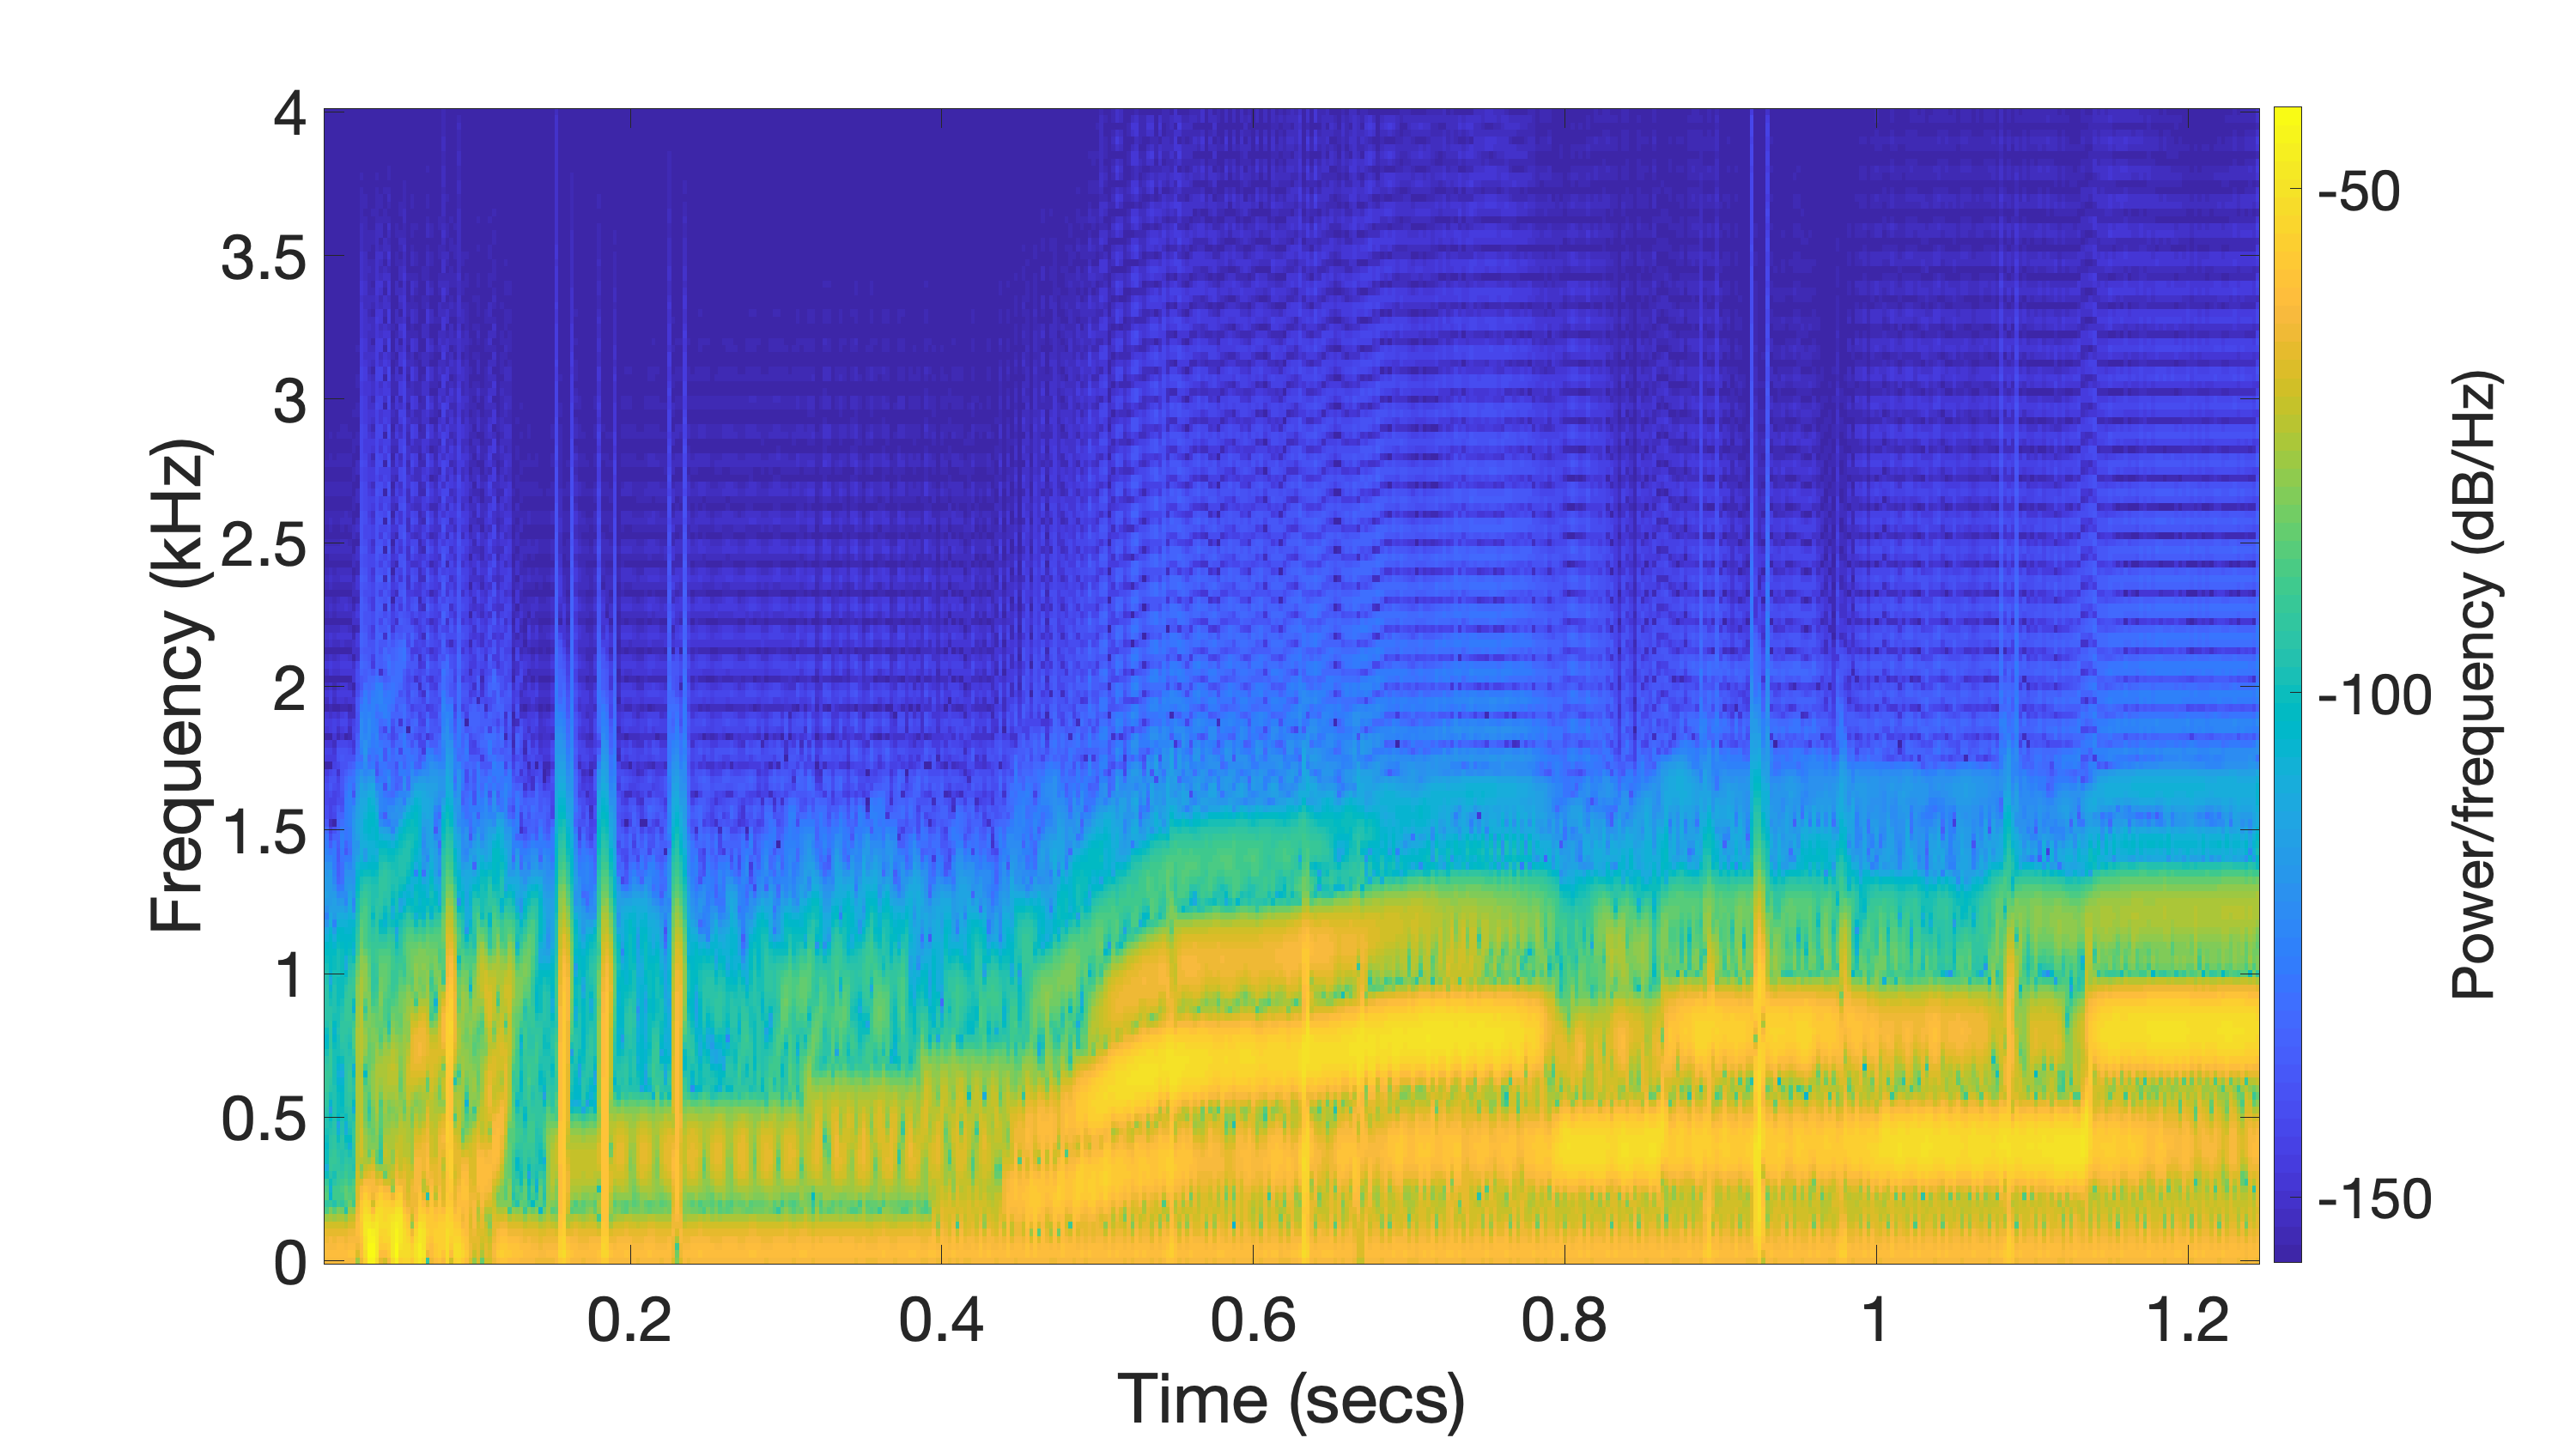
\includegraphics[width= 1.1\textwidth]{figures/R2f_spectrogram.png}
	\caption{Spectrogram of the filtered signal the segment of Fig. \ref{fig:R1b}.}
	\label{fig:R2f_spectrogram}
\end{minipage}
\end{figure}

\section{R3. Filtering with a median filter}

\subsection{R3.a) Median filters}

For an input $x(n)$, the output of a median filter of order $2 M + 1$, where $M \in \mathbb{N}$, is
\begin{equation}
    y(n) = \mathrm{median} \left [ x(n-M), x(n-M+1), ..., x(n+M) \right ].
\end{equation}
This filter is not causal, since its output at discrete time $n$ is dependent on future samples of the input, for instance, at discrete time $n+M$. This means that there is an imposed inferior limit on the delay of the filter when used online. In this case, only after the input at discrete time $n+M$ is given to the filter, it can compute the output at discrete time $n$. In addition, the filter is not linear since the median of a set of real numbers is not a linear operator. This can be shown considering, for instance, a counter-example with the signals $x_1(n) = - \delta(n) - 2 \delta(n-1)$, $x_2(n) = 3 \delta(n) + 5 \delta(n-1) + 9 \delta(n-2)$, and their sum. Nevertheless, the filter is stable in the sense of BIBO stability, since for every bounded input x(n) its median of any order will be bounded. On the other hand, the filter is also time invariant since the median is relative to the discrete time $n$ which means that a time shift in the input signal would shift the output signal in time by the same value.

\subsection{R3.b) Filtered signal and analysis in the time domain}

A median filter of order 3 was also applied to the signal from the sound file \texttt{fugee.wav}. In Fig. \ref{fig:comp_median_zoom_out}-\ref{fig:comp_median_zoom_in}, the comparison of the median filtered signal and the original signal is shown in the time domain for various segments of the song. In the first place, it is possible to observe in Fig. \ref{fig:comp_median_zoom_out} that the noise impulses are completely attenuated in relation to the original signal. This is expected since the impulses are compared to the samples at their sides and one of those is chosen instead of them for the output of the filter. Moreover, one can observe that the rest of the signal is not very attenuated by the filter. In Fig. \ref{fig:comp_median_zoom_med}, a closer representation of the signal in the time domain is depicted. In this case, it is possible to observe that the signal is not very distorted in relation to the original and that the delay of the filter is indistinguishable, which is expected since the response was computed offline. Finally, in Fig. \ref{fig:comp_median_zoom_in}, an even closer depiction of the signal is presented. It is now possible to observe that the signal is clearly distorted in relation to the original one.

\begin{figure}[htbp]
	\begin{minipage}[b]{.49\textwidth}
		\centering
		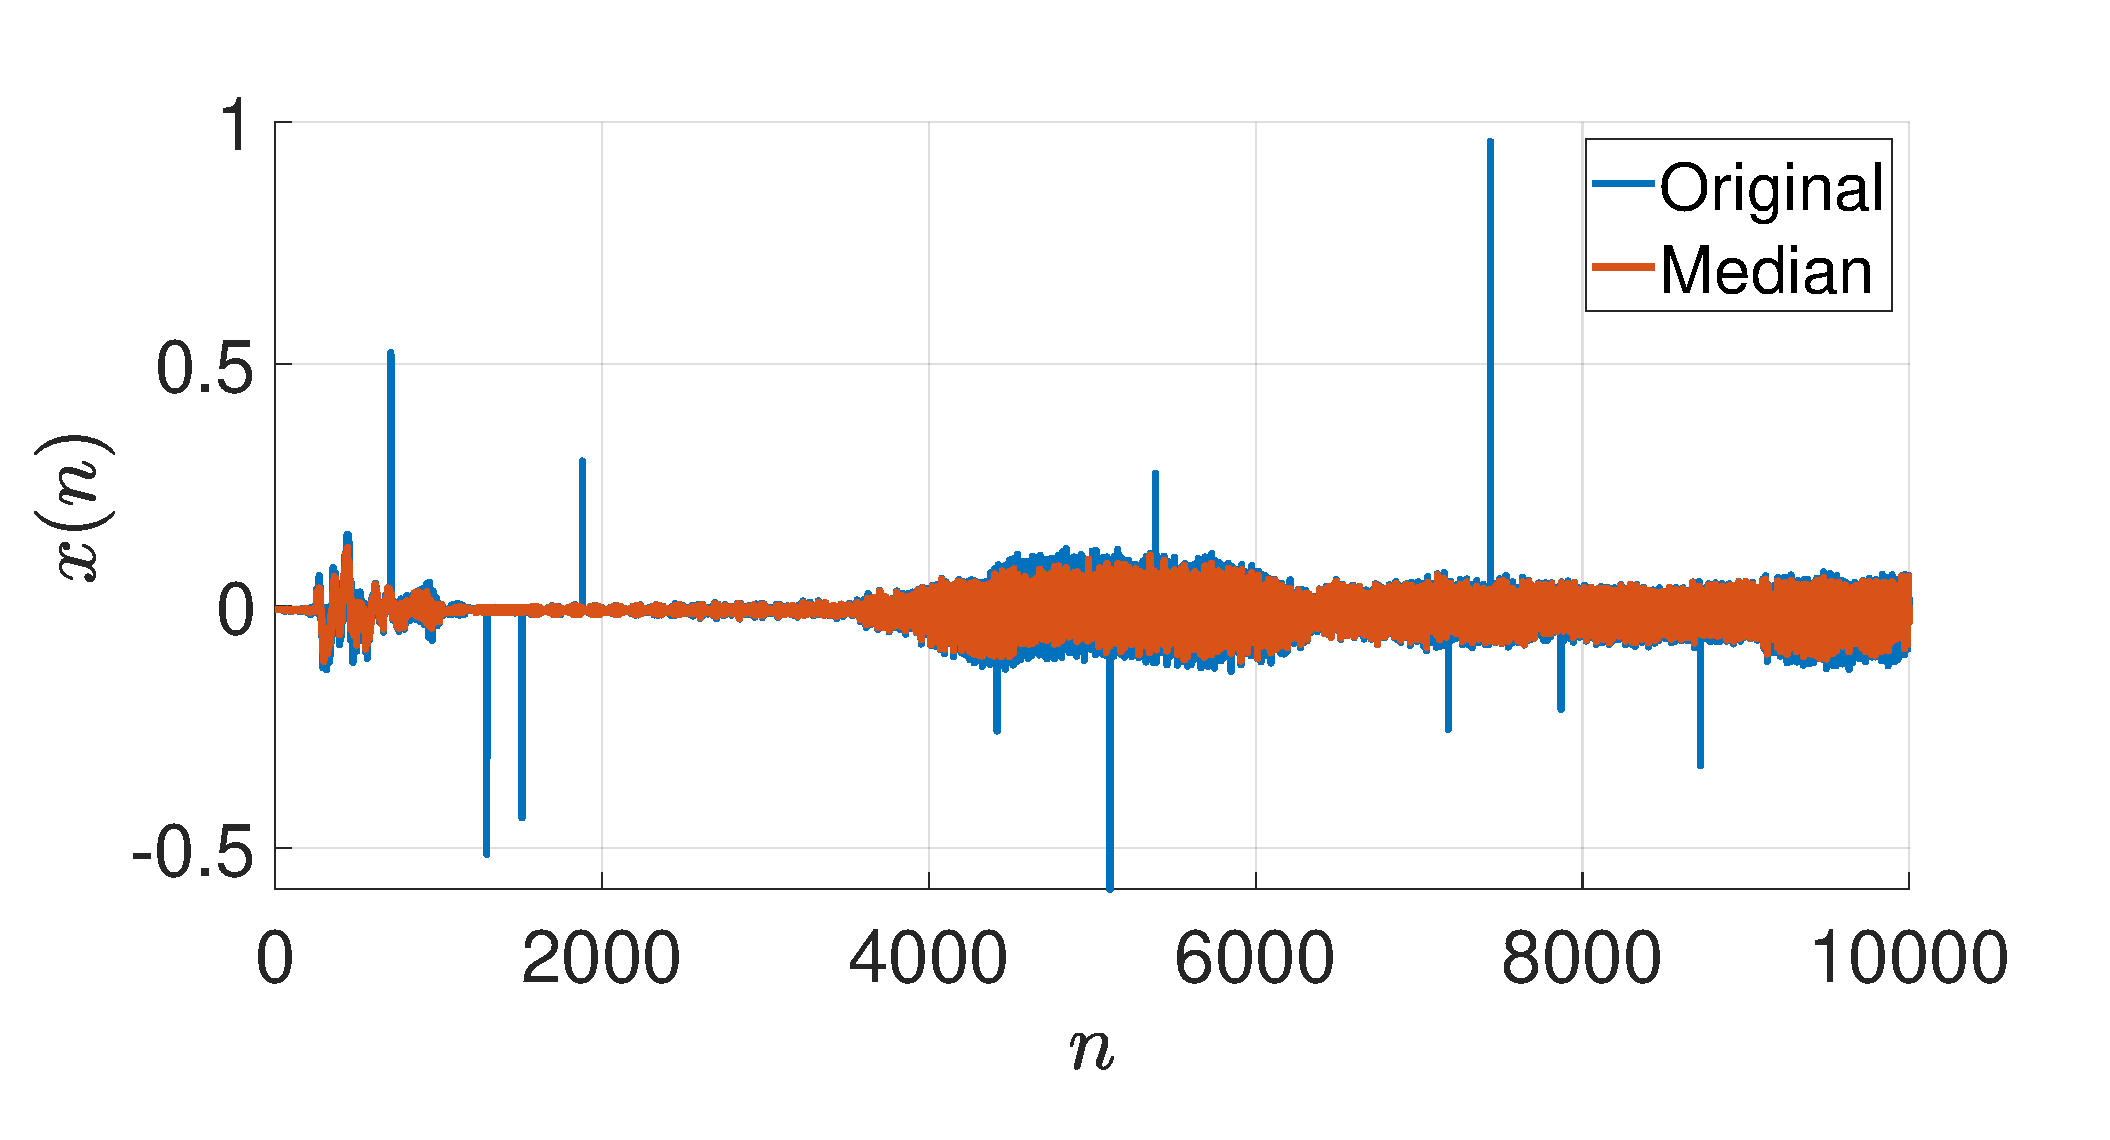
\includegraphics[width= 1.1\textwidth]{figures/comp_median_zoom_out.pdf}
		\caption{Third order median filtered signal.}
		\label{fig:comp_median_zoom_out}
	\end{minipage}
	\hfill
	\begin{minipage}[b]{.49\textwidth}
		\centering
		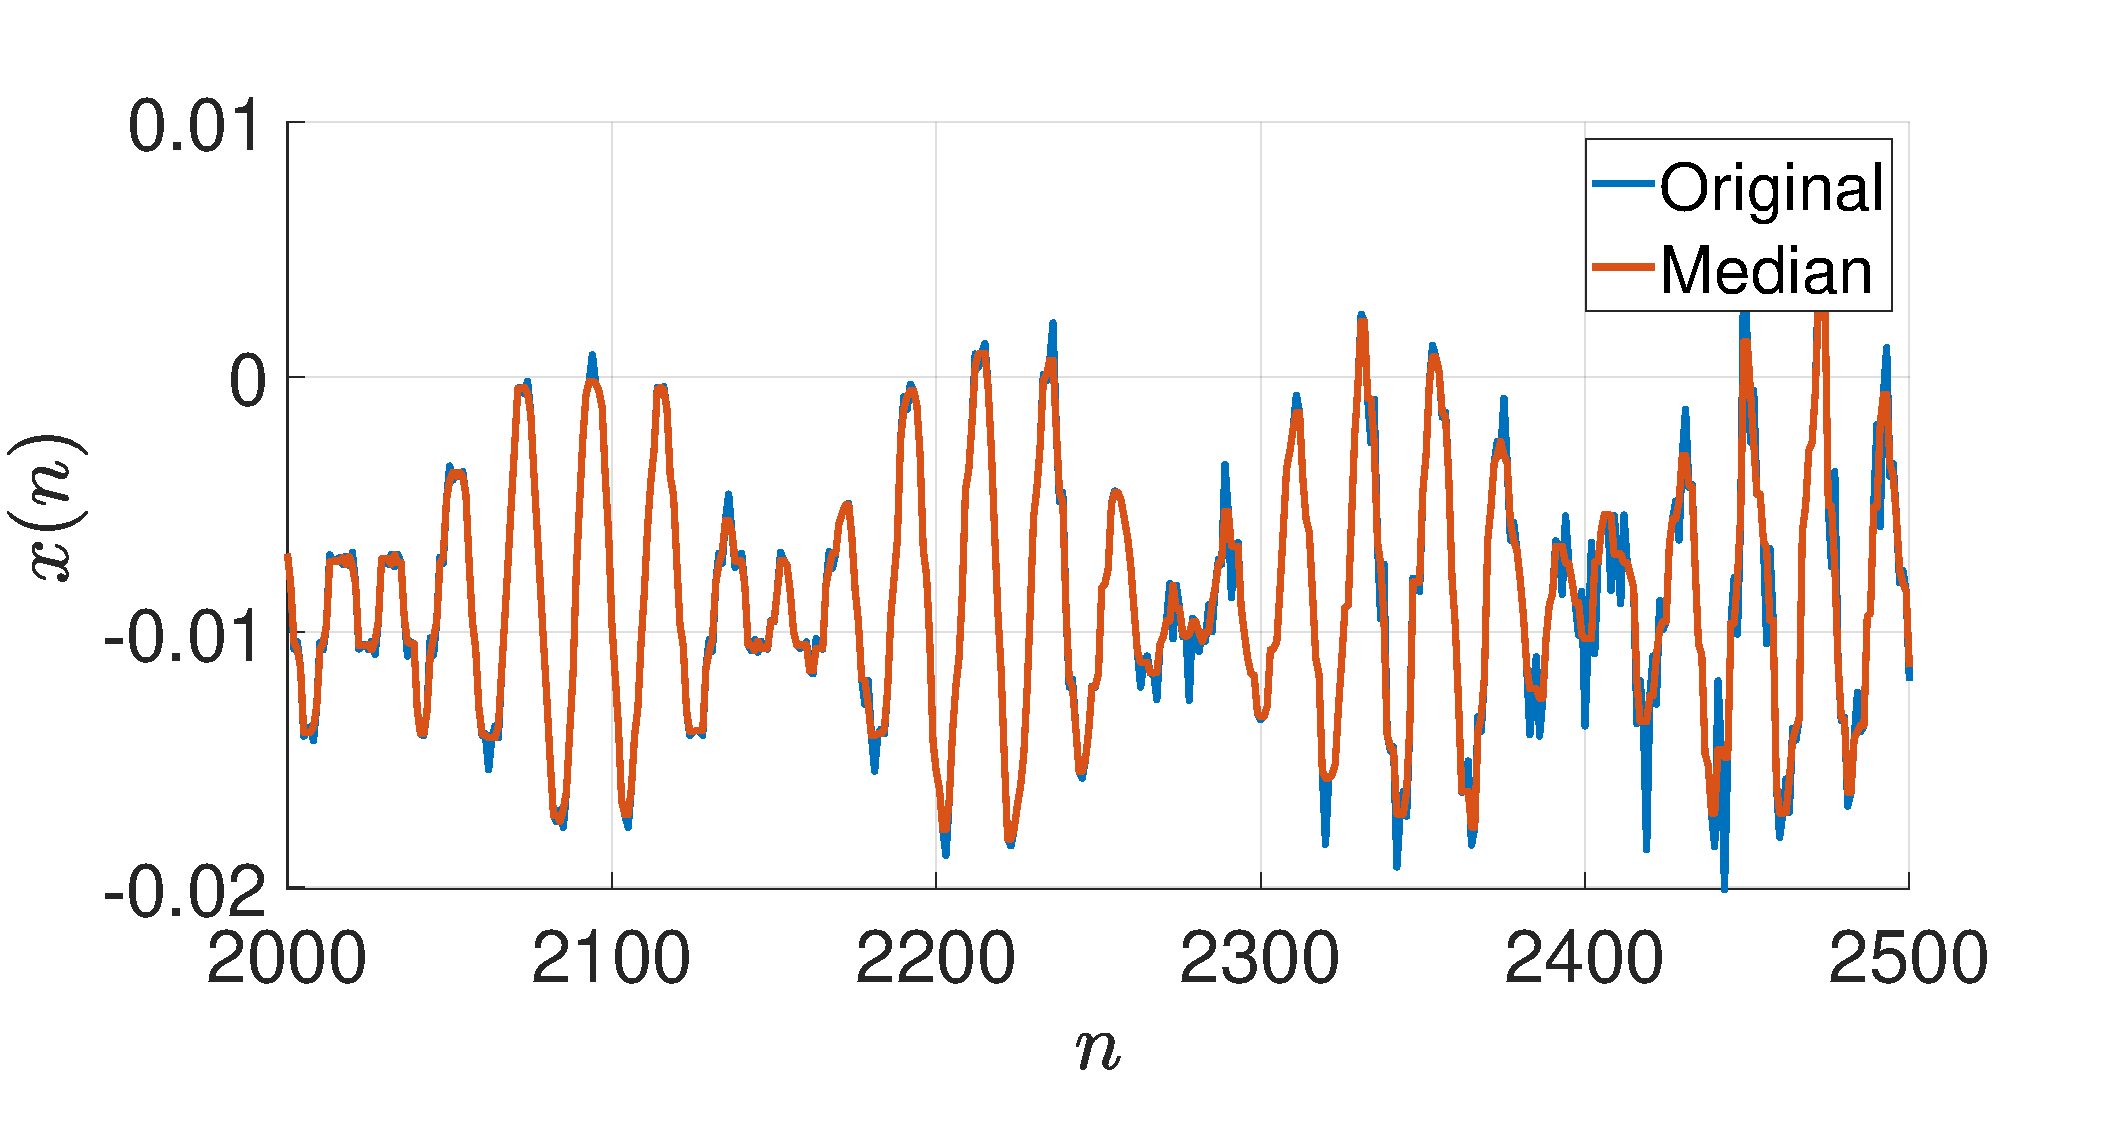
\includegraphics[width= 1.1\textwidth]{figures/comp_median_zoom_med.pdf}
		\caption{Third order median filtered signal.}
		\label{fig:comp_median_zoom_med}
	\end{minipage}
	\begin{minipage}[b]{.49\textwidth}
		\centering
		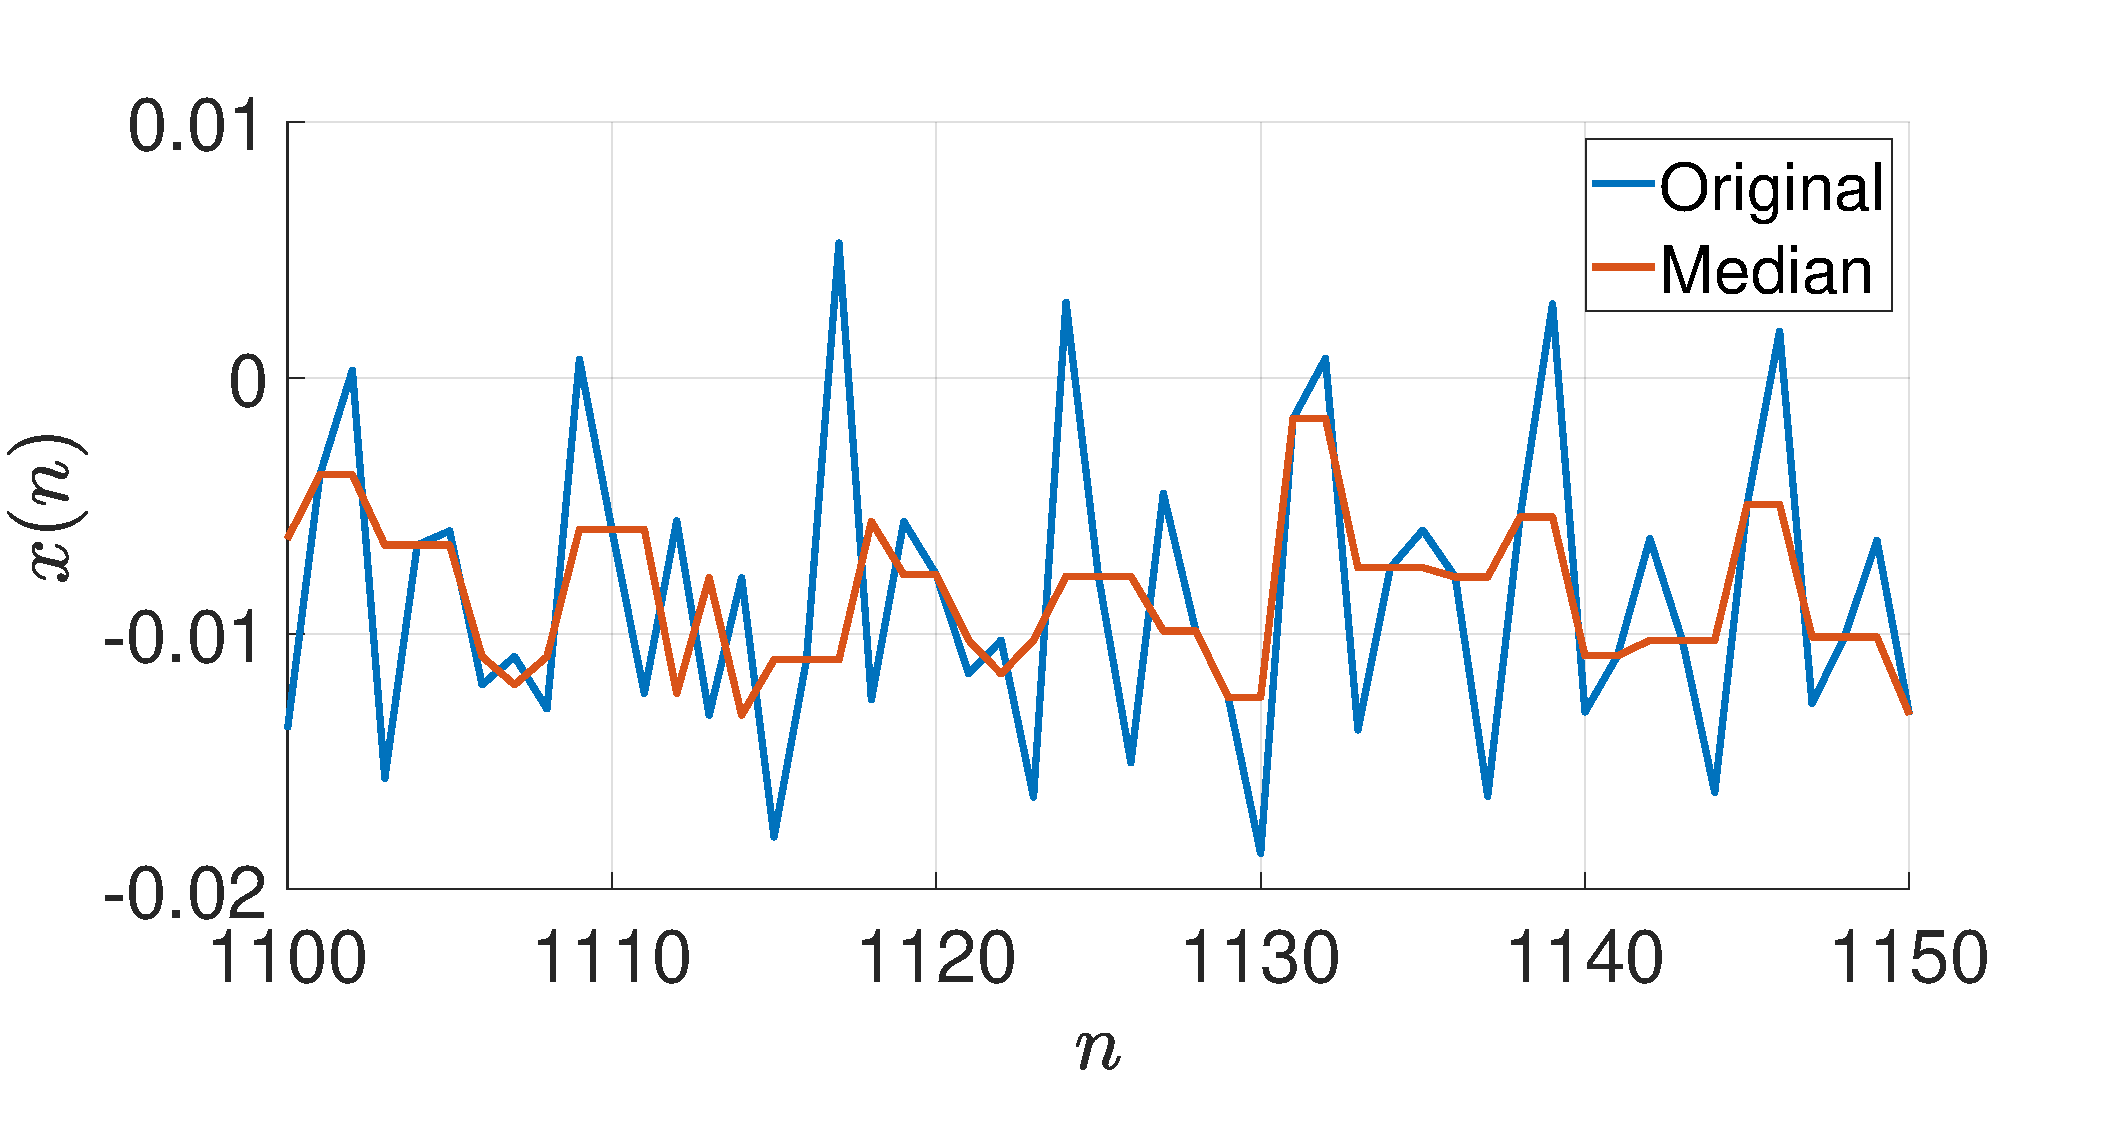
\includegraphics[width= 1.1\textwidth]{figures/comp_median_zoom_in.pdf}
		\caption{Third order median filtered signal.}
		\label{fig:comp_median_zoom_in}
	\end{minipage}
\end{figure}

\subsection{R3.c) Analysis of the filtered signal in the frequency domain}

It is also important to compare the original and the median filtered signal in the frequency domain. In Fig. \ref{fig:dft_comp_median}, the magnitude spectra of the original and filtered signals are represented. It is possible to observe that the attenuation of the filter is only clearly distinguishable for higher frequencies and is not very significant. Given that it is a third order median filter, this result is expected since, beyond the impulses, it also ignores sudden disturbances in the signal for instance. However, the magnitude spectrum is not a good tool to analyze the median filtered signal, since this filter has not a well defined frequency response. In Fig. \ref{fig:spectrogram_median}, a spectrogram of the median filtered signal is again shown for the segment of Fig. \ref{fig:R1b}. It is possible to observe that the higher and lower frequencies were distorted. Comparing the spectrogram of Fig. \ref{fig:spectrogram_median} with the spectrogram of Fig. \ref{fig:R1c_spectrogram}, it is possible to observe that the straight vertical lines corresponding to the impulses are no longer visible which again shows how the impulses have been strongly attenuated.

\begin{figure}[htbp]
	\begin{minipage}[b]{.49\textwidth}
		\centering
		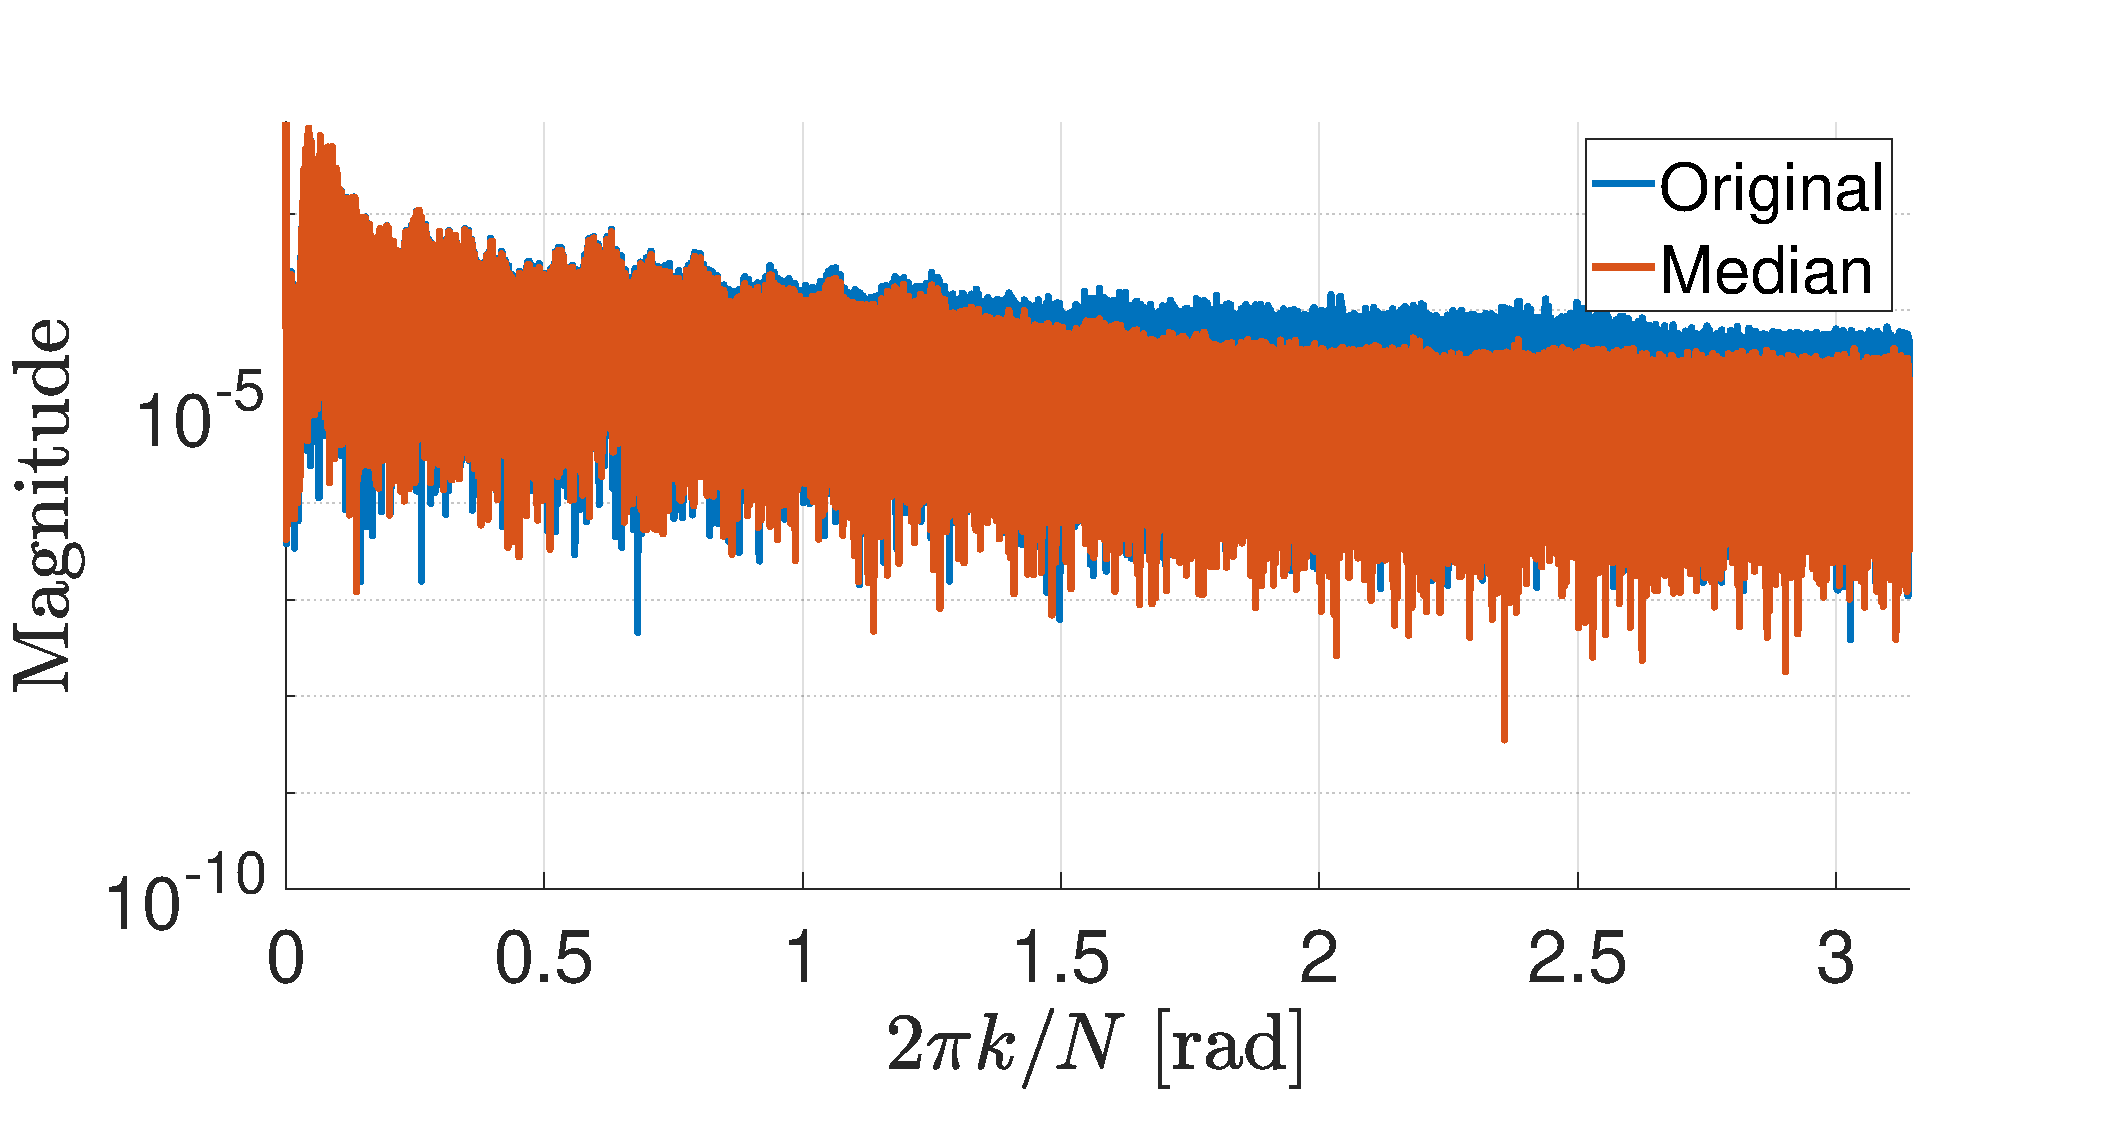
\includegraphics[width= 1.1\textwidth]{figures/dft_comp_median.pdf}
		\caption{Magnitude spectrum of the original and median filtered sound signals.}
		\label{fig:dft_comp_median}
	\end{minipage}
	\hfill
	\begin{minipage}[b]{.49\textwidth}
		\centering
		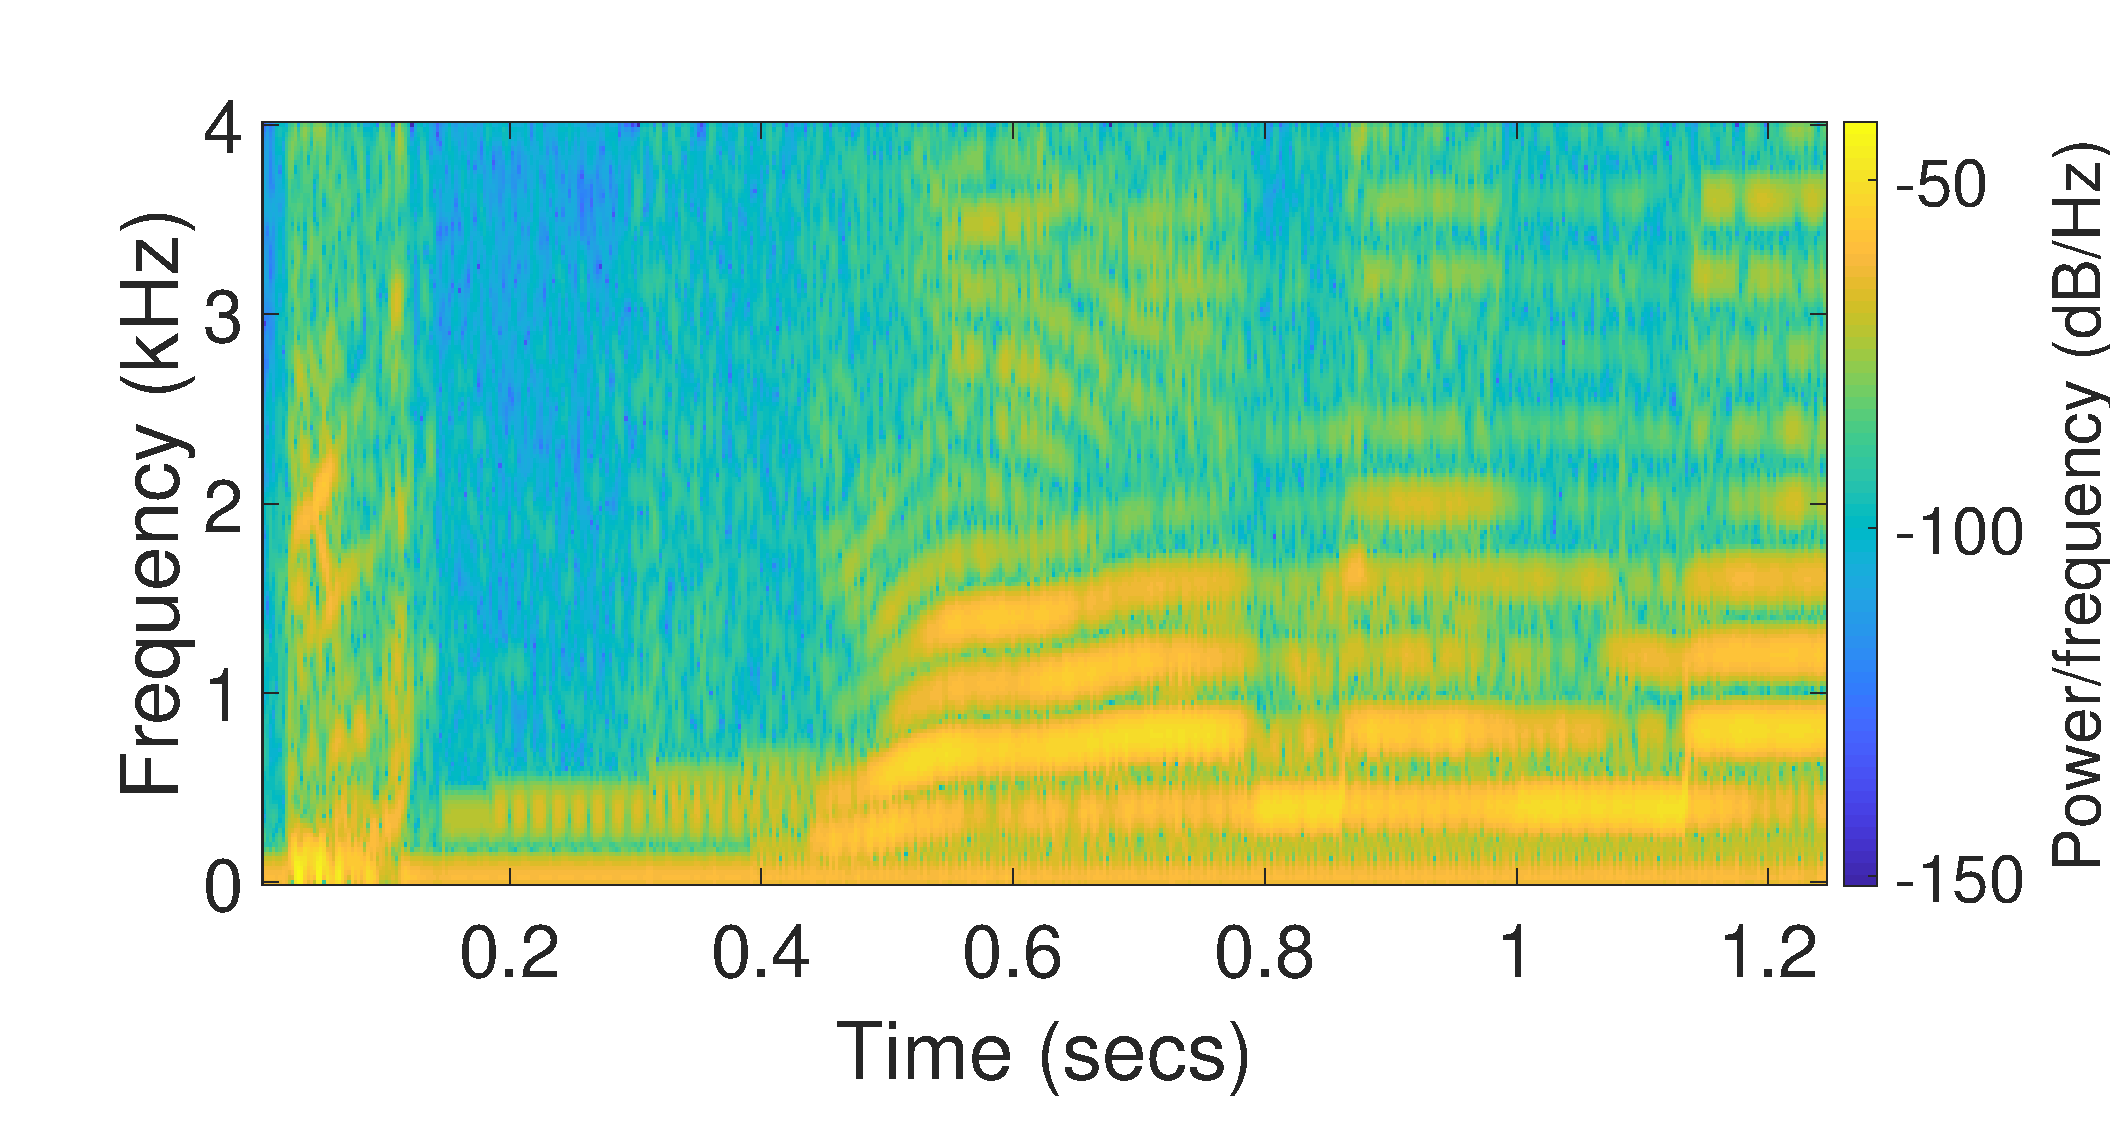
\includegraphics[width= 1.1\textwidth]{figures/spectrogram_median.pdf}
		\caption{Spectrogram of the median filtered signal of the segment of Fig. \ref{fig:R1b}.}
		\label{fig:spectrogram_median}
	\end{minipage}
\end{figure}

\subsection{R3.d) Listening to the filtered signal}

Listening to the median filtered signal it is possible to conclude that the attenuation on the impulsive noise is quite impressive, since it is impossible to distinguish the impulses. However, there was a loss of sharpness in the signal. This loss is considered to be due to the distortion of the higher and lower frequencies.

\subsection{R3.e) Improving median filter}

The minimum order of a median filter is 3. Therefore, in order to find better median filters one has to look for higher order median filters. However, the noise that one wants to remove from this signal is impulsive. Therefore, there is no advantage in using higher order filters. In fact, these filters would just attenuate even more the rest of the signal. In order to experimentally verify this hypothesis, Figs. \ref{fig:comp_median_zoom_out}-\ref{fig:spectrogram_median} were repeated for a seventh order median filter in Fig. \ref{fig:comp_median7_zoom_out}-\ref{fig:spectrogram_median7}. In Fig. \ref{fig:comp_median7_zoom_out} it is clear that the attenuation of the signal increases with this new filter in the time domain. The same goes for the frequency domain as represented in Fig. \ref{fig:dft_comp_median7}, although the attenuation is not so clear in this case. In Fig. \ref{fig:spectrogram_median7}, one can also observe the distortion of the higher and lower frequencies. As in the third order filter, this is the reason why the signal has increased distortion.

\begin{figure}[htbp]
	\begin{minipage}[b]{.49\textwidth}
		\centering
		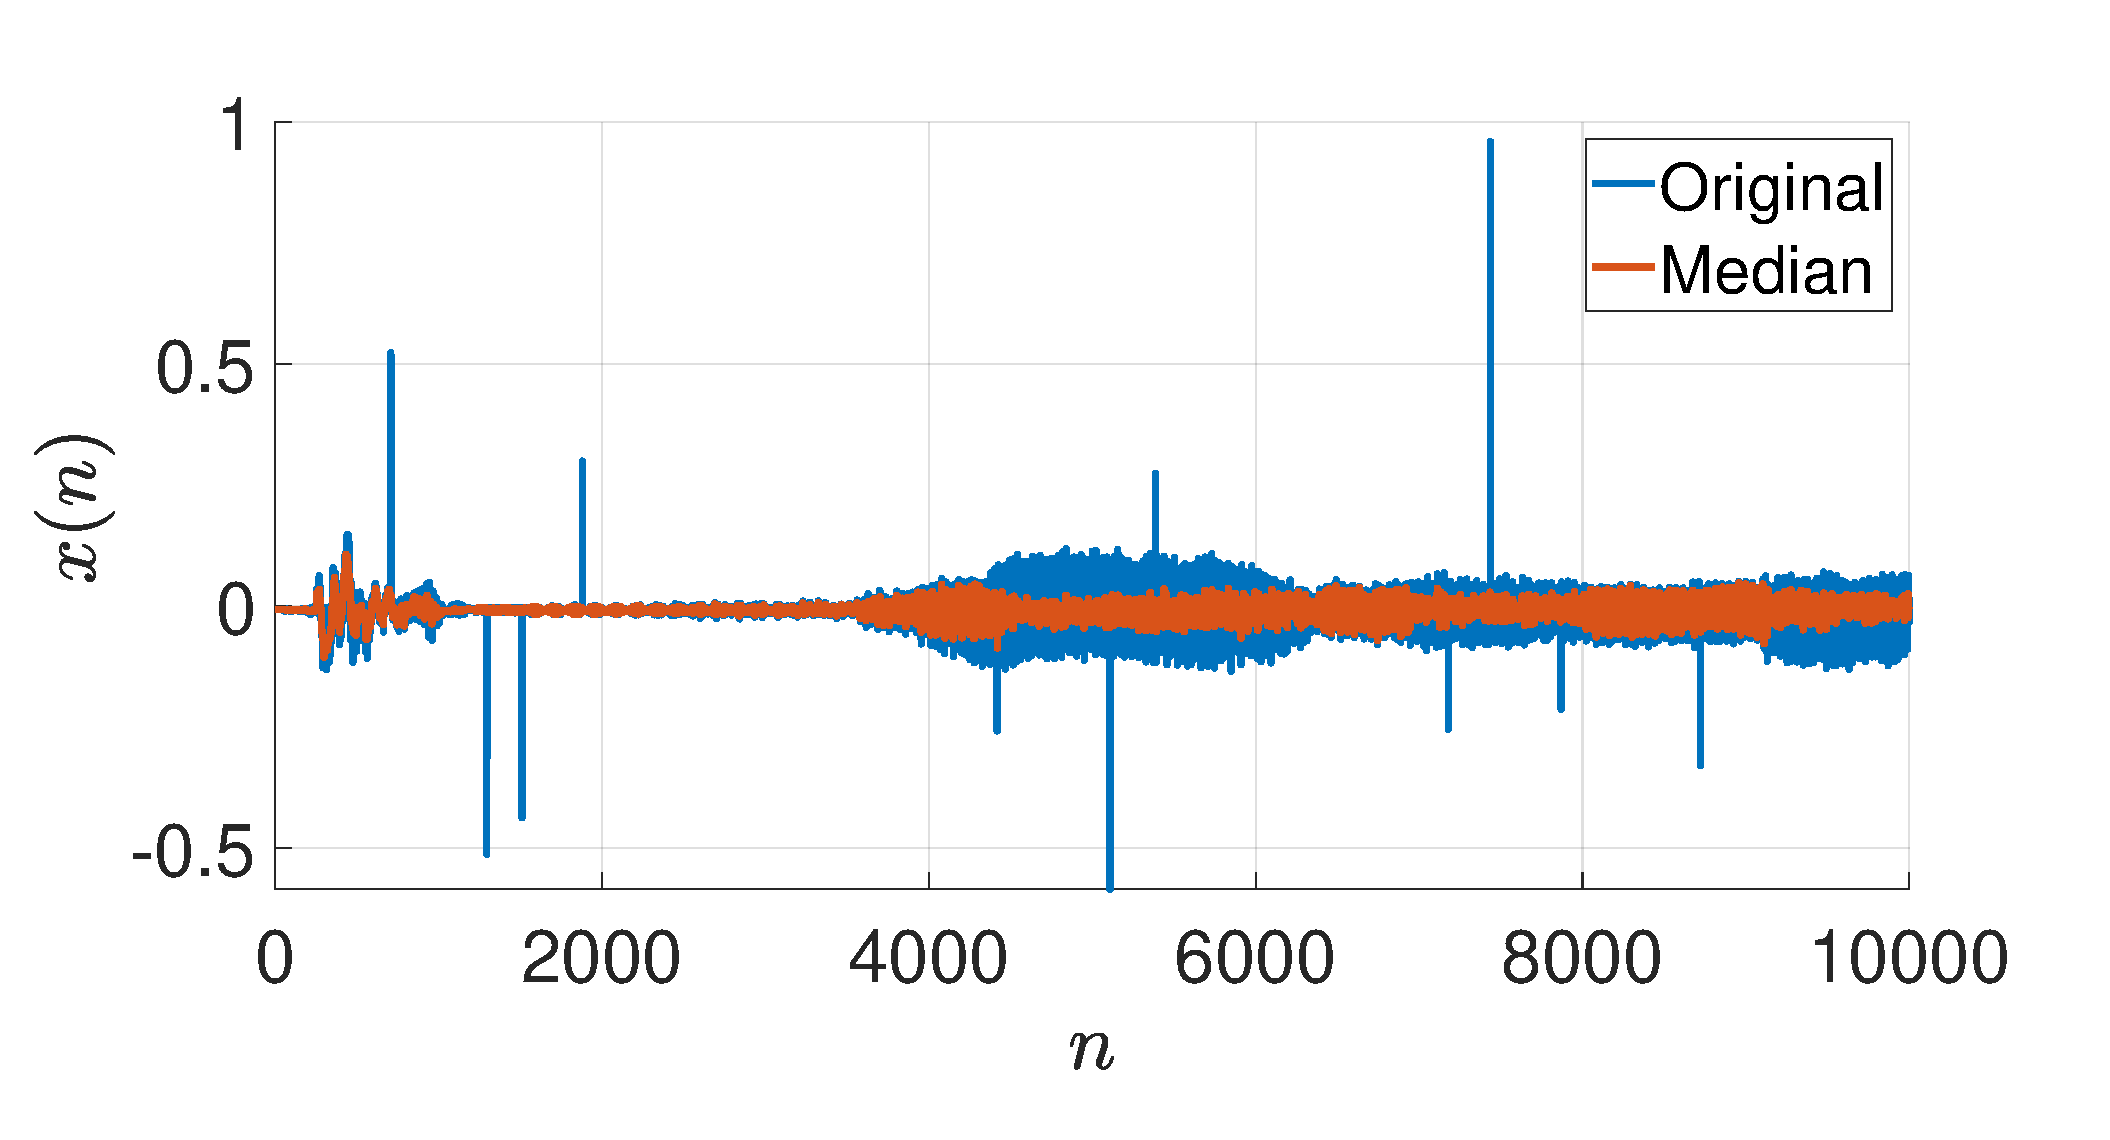
\includegraphics[width= 1.1\textwidth]{figures/comp_median7_zoom_out.pdf}
		\caption{Seventh order median filtered signal.}
		\label{fig:comp_median7_zoom_out}
	\end{minipage}
	\hfill
	\begin{minipage}[b]{.49\textwidth}
		\centering
		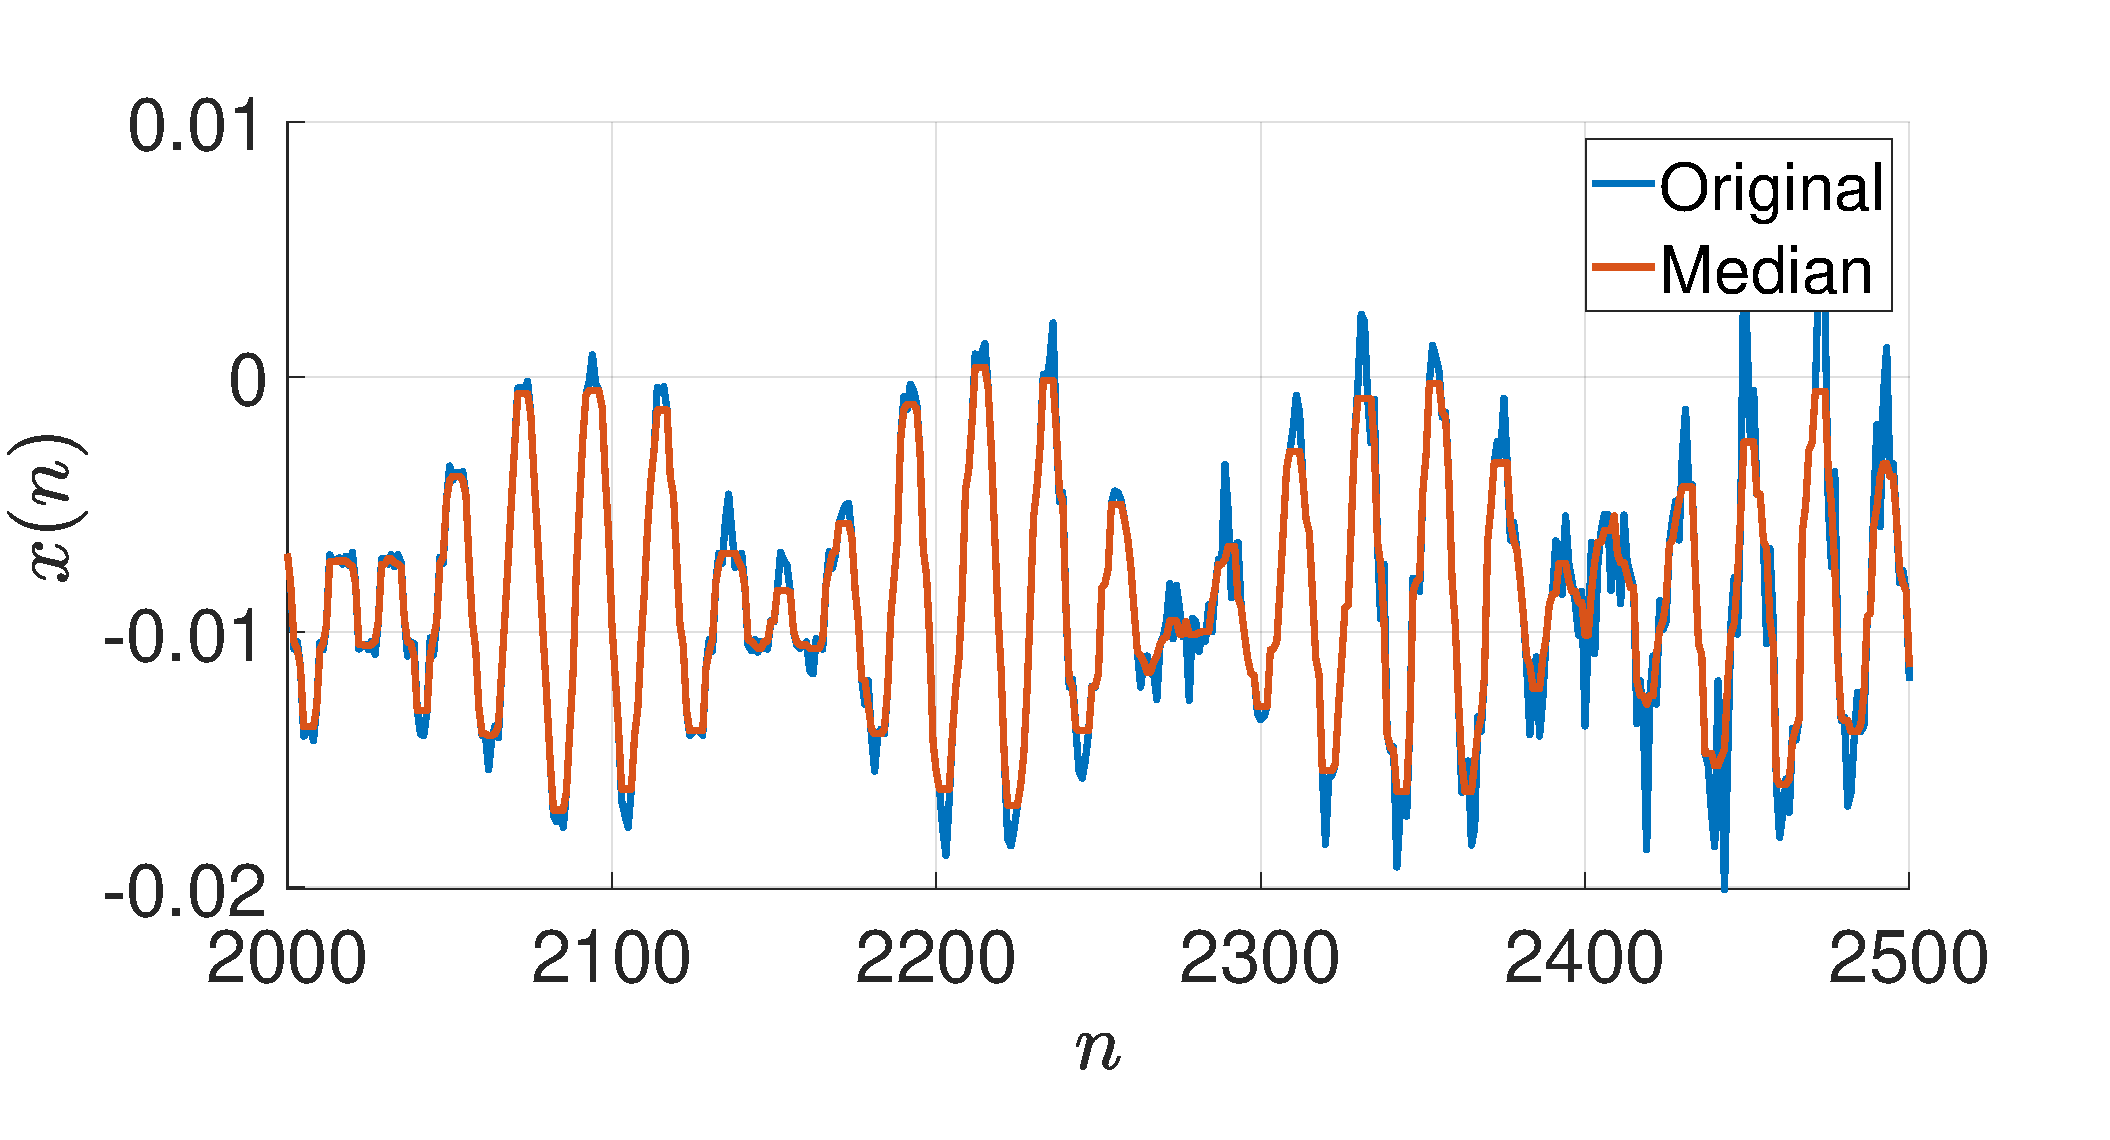
\includegraphics[width= 1.1\textwidth]{figures/comp_median7_zoom_med.pdf}
		\caption{Seventh order median median filtered signal.}
		\label{fig:comp_median7_zoom_med}
	\end{minipage}
	\begin{minipage}[b]{.49\textwidth}
		\centering
		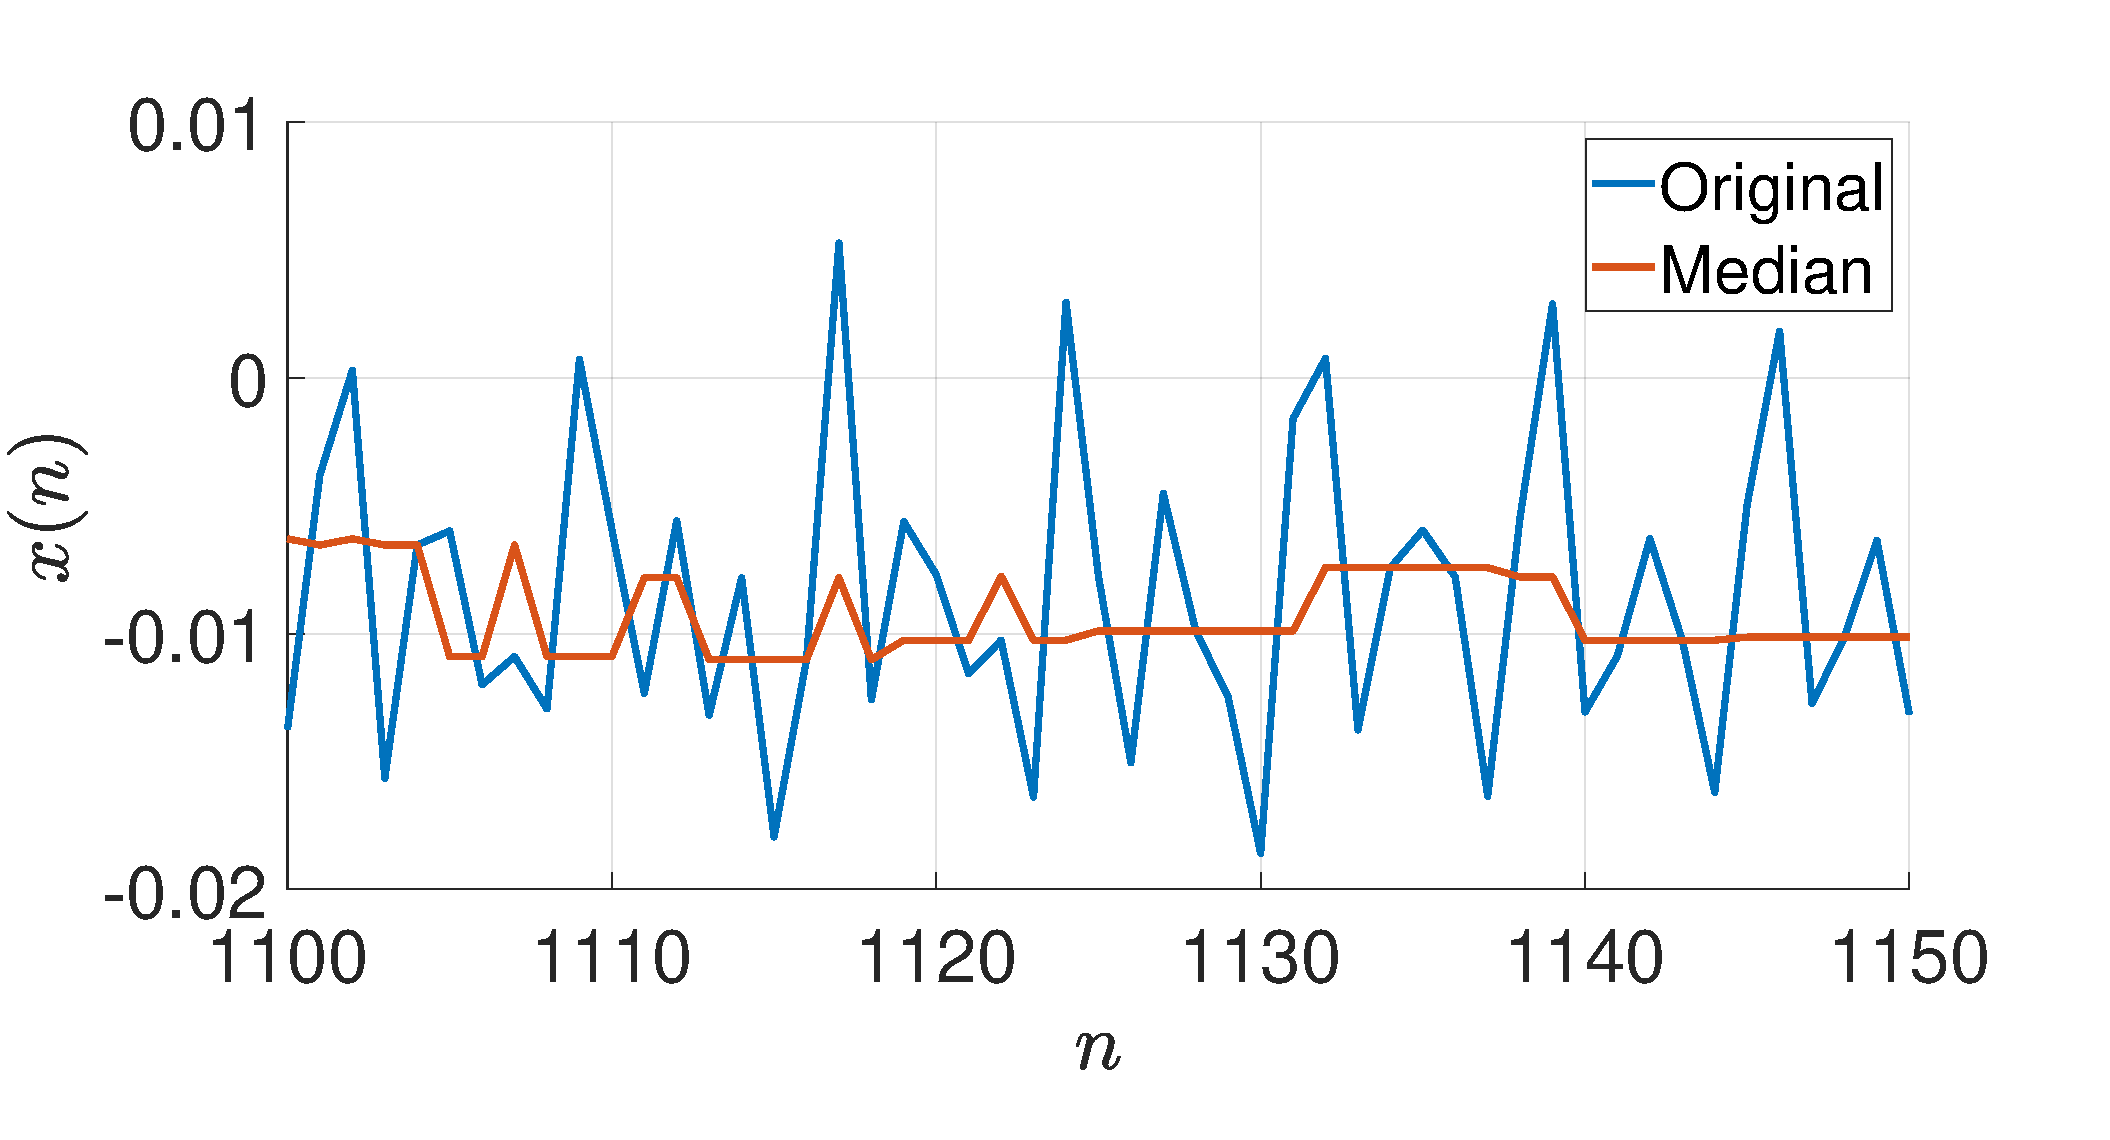
\includegraphics[width= 1.1\textwidth]{figures/comp_median7_zoom_in.pdf}
		\caption{Seventh order median median filtered signal.}
		\label{fig:comp_median7_zoom_in}
	\end{minipage}
	\hfill
	\begin{minipage}[b]{.49\textwidth}
		\centering
		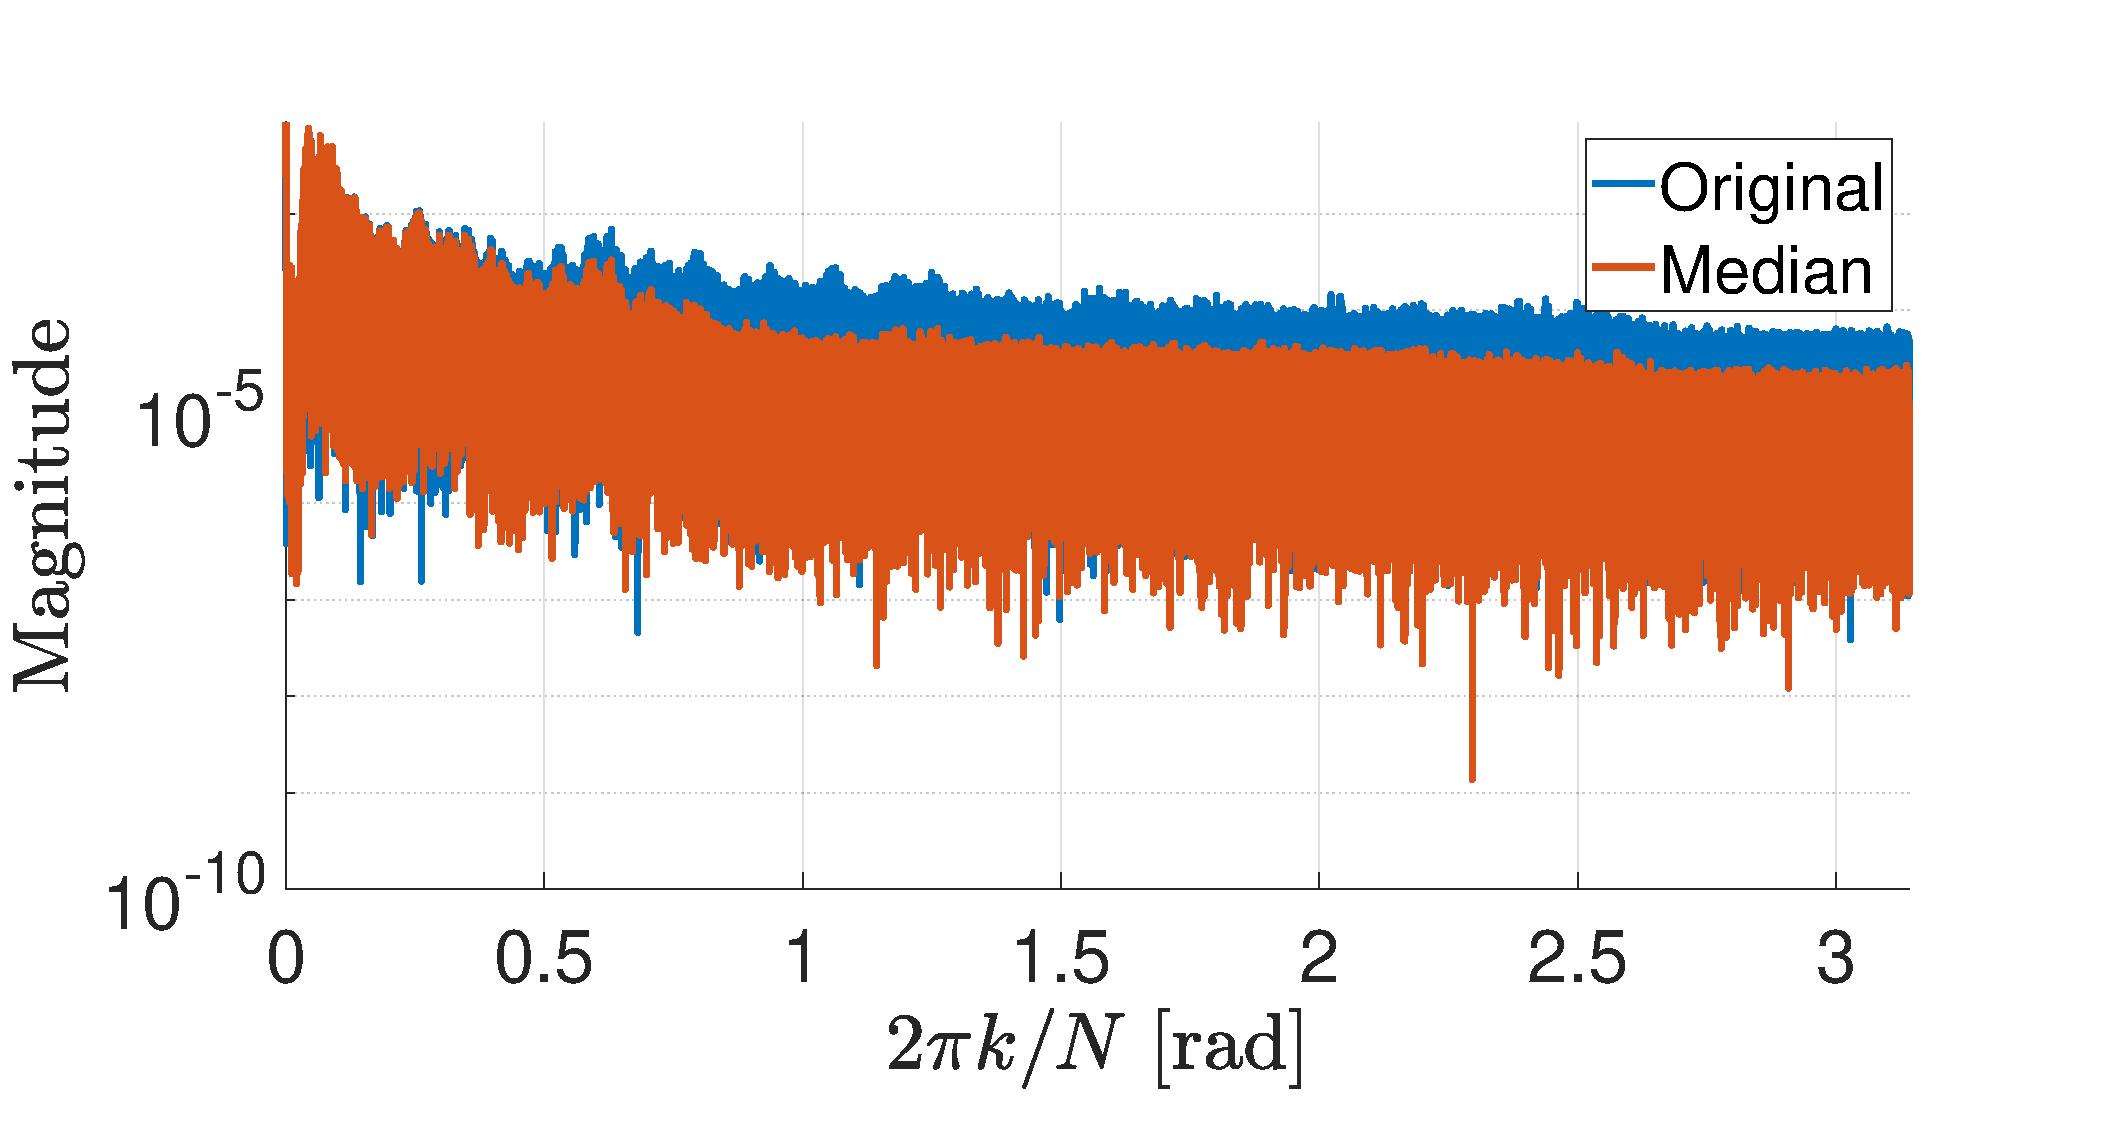
\includegraphics[width= 1.1\textwidth]{figures/dft_comp_median7.pdf}
		\caption{Magnitude spectrum of the original and seventh order median filtered sound signals.}
		\label{fig:dft_comp_median7}
	\end{minipage}
    \begin{minipage}[b]{.49\textwidth}
    	\centering
    	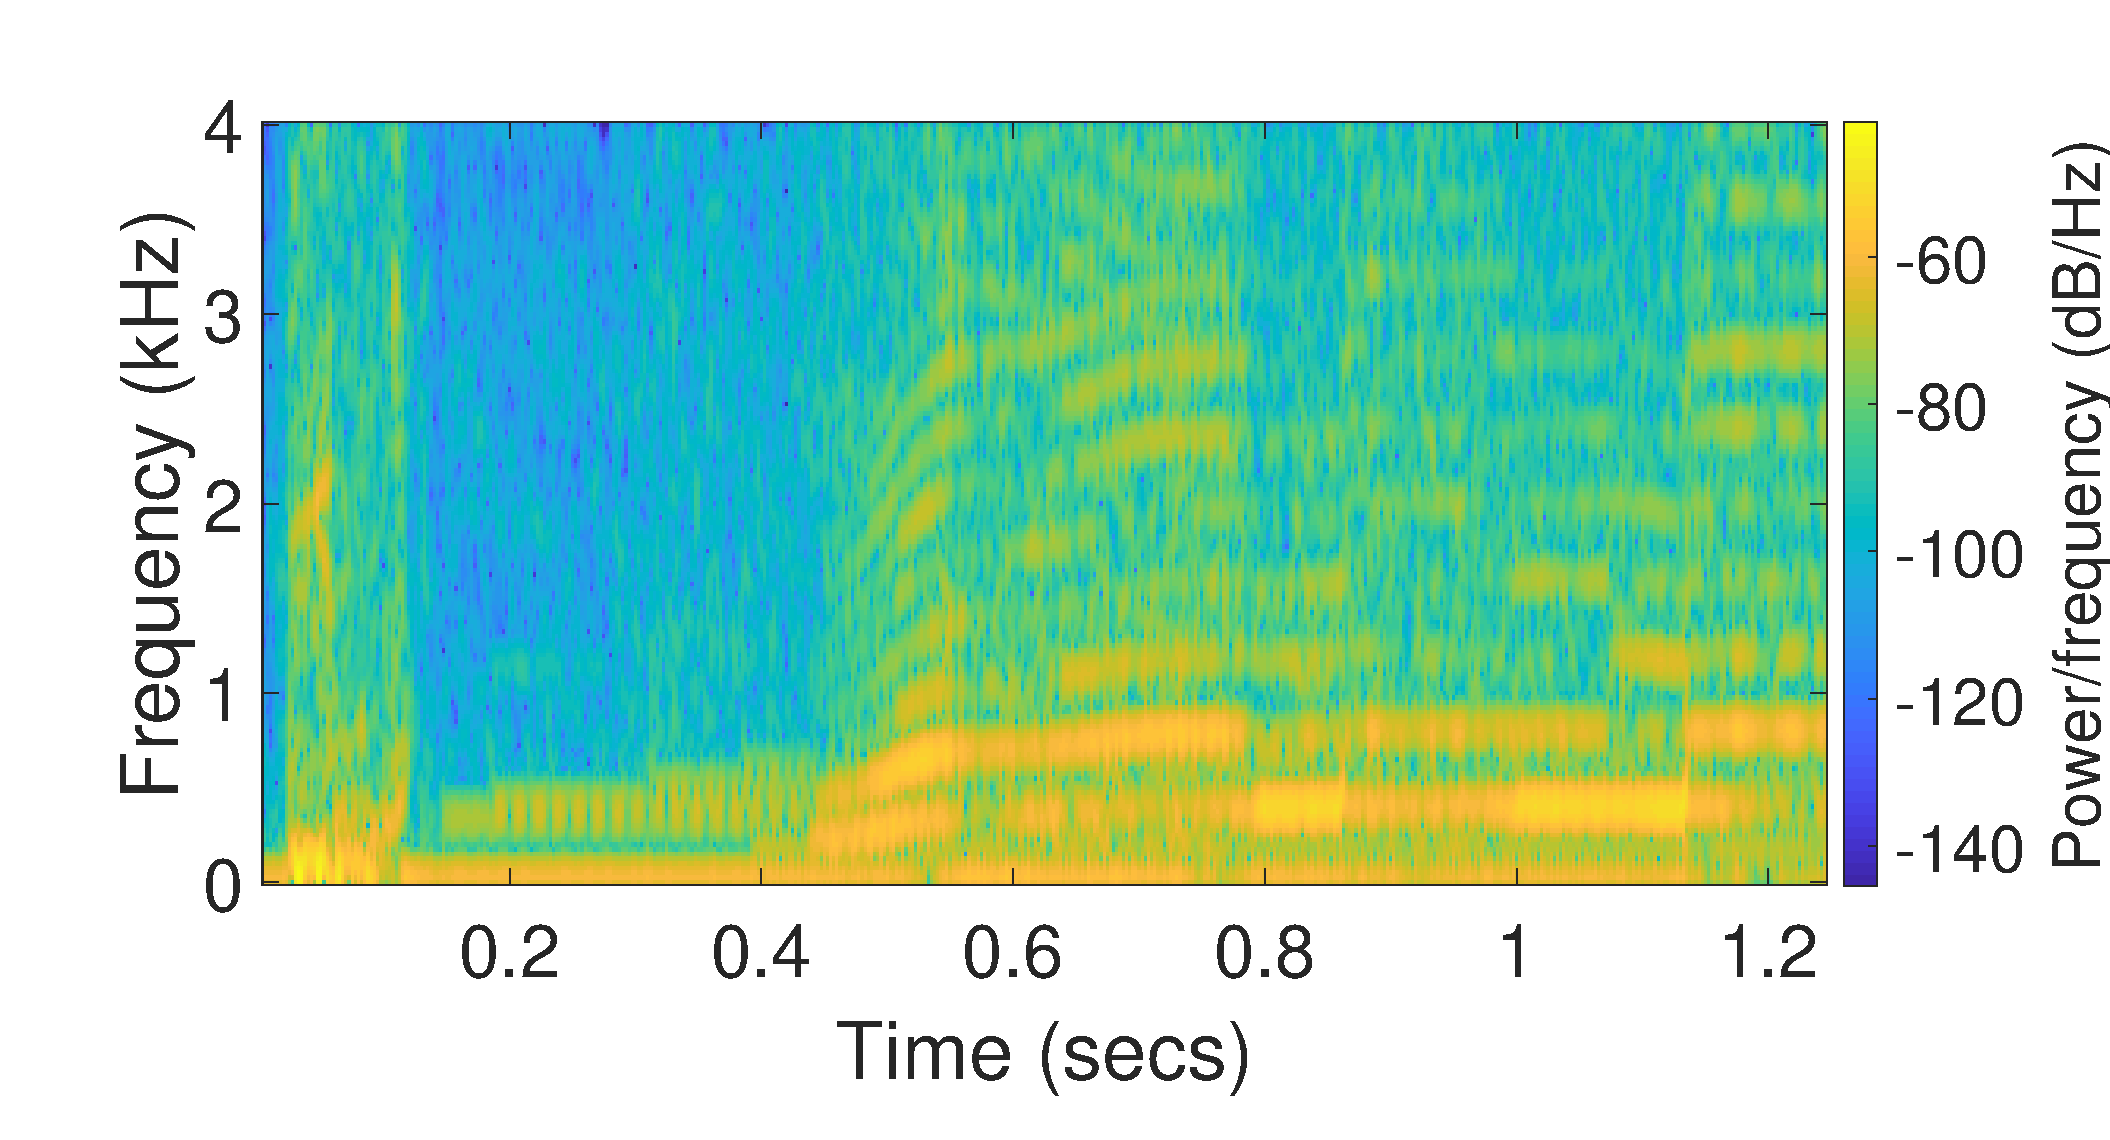
\includegraphics[width= 1.1\textwidth]{figures/spectrogram_median7.pdf}
    	\caption{Spectrogram of the seventh order median filtered signal of the segment of Fig. \ref{fig:R1b}.}
    	\label{fig:spectrogram_median7}
    \end{minipage}
\end{figure}

\subsection{R3.f) Conclusion}

In this work, a recording of the song \textit{Killing Me Softly With His Song} by \textit{Fugees} was analyzed. This recording was corrupted by impulsive noise, which is common in old vynil records. The purpose of the several steps taken was to compare the quality of the filtering obtained with a LTI filter, in this case a Butterworth filter, and a median filter. 

It was observed that the behaviour of the Butterworth filter was not adequate. It did not attenuate efficiently the impulses and attenuated the higher frequencies of the uncorrupted signal, since it has a low-pass frequency response and impulses are all-pass signals. In addition, it had an oscillatory response to the impulsive noise which further decreased the quality of its filtering.

On the other hand, the median filter accurately eliminated the impulsive noise without a significant attenuation of the signal. The biggest disadvantage found of this filter was that it created additional noise which was associated with the distortion of the higher and lower frequencies. It was also observed that the order of the median filter should be in line with the length of the impulses since, for instance, in this case a median of third order was the best option to eliminate the impulses of length one of the signal. However, in real situations the impulsive noise will not have a definite length, which means that a deeper analysis of the order of the median filter is needed.

\end{document}

